\newif\ifanonymous
\newif\iftitlepageonly
\newif\ifannotated
\newif\ifshowstubs \showstubsfalse%
\newif\ifsnjnl \snjnlfalse
\ifdefined\anonrender \anonymoustrue \fi
\ifdefined\titlepagerender \titlepageonlytrue \fi
\ifdefined\annotatedrender \annotatedtrue \fi
\ifdefined\hidestubsrender \showstubsfalse \fi\ifdefined\showstubsrender \showstubstrue \fi
\ifsnjnl
  \documentclass[pdflatex,sn-basic]{sn-jnl}%
\else
  \documentclass[11pt,a4paper]{article}
\fi

\ifsnjnl
\else
  \usepackage[T1]{fontenc}
  \usepackage{lmodern}
  \usepackage[a4paper,margin=2.5cm]{geometry}
  \usepackage[authoryear,round]{natbib}
  \usepackage[title]{appendix}
  \usepackage{microtype}
  \usepackage{caption}
  \captionsetup[table]{position=top,skip=6pt}
  \providecommand{\bmhead}[1]{\paragraph*{#1}}
  \providecommand{\backmatter}{}
  \newcommand{\keywords}[1]{\par\medskip\noindent\textbf{Keywords:} #1\par}
\fi

\usepackage{amsmath,amssymb}
\usepackage{graphicx}
\usepackage[table]{xcolor}
\usepackage{array,booktabs,tabularx}
\usepackage{rotating}   %
\usepackage{placeins}   %
\usepackage{enumitem}
\usepackage{tikz}
\usetikzlibrary{arrows.meta,positioning,calc,shapes.misc}
\renewcommand{\topfraction}{.85}\renewcommand{\floatpagefraction}{.75}\renewcommand{\textfraction}{.1}\makeatletter\setlength{\@fptop}{0pt}\makeatother%
\newcommand{\tablerows}{\renewcommand{\arraystretch}{1.6}}%
\usepackage{hyperref}
\usepackage{orcidlink}
\makeatletter\g@addto@macro\UrlBreaks{\do\-\do\:}\makeatother%
\hypersetup{hidelinks}
\hypersetup{pdftitle={Aligning AI Requires Aligning with Each Other: A Covenant}}
\ifanonymous\else\hypersetup{pdfauthor={Ioannis Tsiokos}}\fi

% Generated by scripts/paper_set_release.py.
\newif\ifpaperhasdoi
\paperhasdoitrue
\newcommand{\paperdoi}{10.5281/zenodo.23413556}
\newcommand{\manuscriptversion}{Preprint v1.0}
\newcommand{\manuscriptdate}{16 October 2026}
\newcommand{\manuscriptyear}{2026}

\newcommand{\releasefooter}{\scriptsize Automorph Inc.\enspace ioannis@automorph.io\enspace\ifpaperhasdoi DOI: \href{https://doi.org/\paperdoi}{\paperdoi}\enspace\fi\textcopyright\ \manuscriptyear\enspace CC-BY 4.0\enspace Preprint, not peer reviewed.}
\ifanonymous\else\ifsnjnl\else
  \usepackage{fancyhdr}
  \setlength{\footskip}{36pt}
  \fancypagestyle{plain}{\fancyhf{}\renewcommand{\headrulewidth}{0pt}\fancyfoot[C]{\thepage\\[3pt]\releasefooter}}
  \pagestyle{plain}
\fi\fi

\newcommand{\numLeanDecls}{127} %
\newcommand{\numLeanDEighteenDecls}{69} %
\newcommand{\numLeanDEighteenFiles}{8} %
\newcommand{\numLeanDEighteenGeneric}{31} %
\newcommand{\numLeanDEighteenControls}{15} %
\newcommand{\numLeanDEighteenSpecialized}{23} %
\newcommand{\numLeanCarrier}{5} %
\newcommand{\numLeanRolePrivacy}{10} %
\newcommand{\numLeanPayoffsDOne}{1} %
\newcommand{\numLeanPayoffsDTen}{3} %
\newcommand{\numLeanPayoffsDEleven}{3} %
\newcommand{\numLeanHorizon}{3} %
\newcommand{\numLeanDecoding}{5} %
\newcommand{\numLeanRecovery}{8} %
\newcommand{\numLeanAssessment}{7} %
\newcommand{\numLeanDependence}{6} %
\newcommand{\numLeanAdoption}{8} %
\newcommand{\numLeanCoalitions}{7} %
\newcommand{\numLeanControlGroups}{5} %
\newcommand{\numLeanEvidence}{10} %
\newcommand{\numVTenNotAdmitted}{464} %
\newcommand{\numVTenAdmitted}{944} %
\newcommand{\numVTenCompatible}{1{,}408} %
\newcommand{\numInstSplitWitnesses}{48} %
\newcommand{\numInstStrictRounds}{3--6} %
\newcommand{\numInstValidators}{33} %
\newcommand{\numInstCoincideRounds}{1--2} %
\newcommand{\numInstAllRows}{36} %
\newcommand{\numInstFormationRows}{24} %
\newcommand{\numInstFormedRows}{12} %
\newcommand{\numInstLoopPairs}{512} %
\newcommand{\numInstLoopPairsLate}{352} %
\newcommand{\numInstLoopPairsEarly}{160} %
\newcommand{\numGlassSpins}{8} %
\newcommand{\numGlassHorizons}{1--21} %
\newcommand{\numInstHumanGain}{0.029} %
\newcommand{\numInstEarlyGain}{0.018} %
\newcommand{\numInstLateGain}{0.060} %
\newcommand{\numVOneDefectProfiles}{512} %
\newcommand{\numVOneNonemptyProfiles}{511} %
\newcommand{\numVTenCompilerTrustDecls}{3} %
\newcommand{\numTTPCitedDecls}{82} %
\newcommand{\numFThreeStackBound}{\ensuremath{N\le 1}} %
\newcommand{\numCOneWorlds}{8{,}192} %
\newcommand{\numCOneCommands}{169} %
\newcommand{\numCOneIsolatedFailures}{5} %
\newcommand{\numCNineReceiptCombos}{8} %
\newcommand{\numCFifteenSnapshots}{27} %
\newcommand{\numCFifteenTargets}{17} %
\newcommand{\numCTwoChannels}{16} %
\newcommand{\numDOneEps}{\ensuremath{1/20}} %
\newcommand{\numDOneBenefit}{3} %
\newcommand{\numDOneAlphaKTwo}{\ensuremath{\approx 0.638}} %
\newcommand{\numDOneAlphaKOne}{\ensuremath{\approx 0.380}} %
\newcommand{\numDOneRationalCases}{14} %
\newcommand{\numDSevenCases}{72} %
\newcommand{\numDSevenDeviations}{1{,}296} %
\newcommand{\numDFiveMaxN}{7} %
\newcommand{\numDFiveMaxB}{3} %
\newcommand{\numDNineEndowment}{2} %
\newcommand{\numDNineBudget}{\ensuremath{1/2}} %
\newcommand{\numDTenHosts}{5} %
\newcommand{\numDTenRequired}{2} %
\newcommand{\numDElevenTables}{3} %
\newcommand{\numDEightLaws}{5} %
\newcommand{\numDEightSlackContract}{\ensuremath{10377/32390}} %
\newcommand{\numDEightSlackDonor}{\ensuremath{10377/32390}} %
\newcommand{\numDEightSlackSensor}{\ensuremath{39370816377/129757678790}} %
\newcommand{\numDEightDiscount}{\ensuremath{3/4}} %
\newcommand{\numDEightBenefit}{3} %
\newcommand{\numDEightCost}{1} %
\newcommand{\numDEightEps}{\ensuremath{1/20}} %
\newcommand{\numDEightSensorErr}{\ensuremath{29/4000}} %
\newcommand{\numDEightPrivateCoop}{\ensuremath{902899/1181900}} %
\newcommand{\numDEightPrivateDis}{\ensuremath{11039/59095}} %
\newcommand{\numDEightCommonCoop}{\ensuremath{419/496}} %
\newcommand{\numDEightCommonDis}{\ensuremath{19/248}} %
\newcommand{\numDEightContractCoop}{\ensuremath{127/140}} %
\newcommand{\numDEightContractDis}{0} %
\newcommand{\numDFourteenFamilies}{495} %
\newcommand{\numDFourteenN}{6} %
\newcommand{\numDFourteenA}{2} %
\newcommand{\numDFourteenC}{1} %
\newcommand{\numDFourteenEntry}{\ensuremath{1/10}} %
\newcommand{\numDFourteenSubsidy}{\ensuremath{1/2}} %
\newcommand{\numDFourteenStartPlain}{3} %
\newcommand{\numDFourteenProbPlain}{\ensuremath{1/2}} %
\newcommand{\numDFourteenTimePlain}{10} %
\newcommand{\numDFourteenStartSubsidy}{2} %
\newcommand{\numDFourteenProbSubsidy}{\ensuremath{2/3}} %
\newcommand{\numDFourteenTimeSubsidy}{\ensuremath{31/3}} %
\newcommand{\numDFifteenCCValue}{\ensuremath{627/100}} %
\newcommand{\numDFifteenBindingValue}{\ensuremath{38/5}} %
\newcommand{\numDFifteenResetValue}{\ensuremath{15009170612/2088907793}} %
\newcommand{\numDFifteenBenefit}{3} %
\newcommand{\numDFifteenCost}{1} %
\newcommand{\numDFifteenEps}{\ensuremath{1/20}} %
\newcommand{\numDFifteenPrep}{\ensuremath{1/4}} %
\newcommand{\numDFifteenDiscount}{\ensuremath{3/4}} %
\newcommand{\numDFifteenExcessPrep}{2} %
\newcommand{\numDFifteenFamilies}{729} %
\newcommand{\numDFifteenProfiles}{6{,}561} %
\newcommand{\numDSixteenFamilies}{1{,}458} %
\newcommand{\numDSixteenCartelCases}{27{,}216} %
\newcommand{\numDSixteenCoalitionCases}{54} %
\newcommand{\numDSixteenFactGroups}{5} %
\newcommand{\numDSixteenCapacities}{5} %
\newcommand{\numDSixteenAliases}{5} %
\newcommand{\numDTwentyThreeWords}{254} %
\newcommand{\numDTwentyThreeWordLengths}{1--7} %
\newcommand{\numDTwentyThreeCurrentErr}{\ensuremath{1/20}} %
\newcommand{\numDTwentyThreeNextErr}{\ensuremath{13/80}} %
\newcommand{\numDTwentyThreeObsErr}{\ensuremath{1/20}} %
\newcommand{\numDTwentyThreeRho}{\ensuremath{1/4}} %
\newcommand{\numDTwentyThreePrior}{\ensuremath{1/2}} %
\newcommand{\numDTwentyThreeGradeEps}{\ensuremath{1/20}} %
\newcommand{\numDTwentyThreeGamma}{\ensuremath{1/2}} %
\newcommand{\numDTwentyThreeK}{2} %
\newcommand{\numDNineteenStates}{24} %
\newcommand{\numDNineteenInterests}{15} %
\newcommand{\numDNineteenPhaseComparisons}{310{,}272} %
\newcommand{\numDNineteenQuotes}{96} %
\newcommand{\numDNineteenMinSurplus}{\ensuremath{377/4}} %
\newcommand{\numDTwentyCash}{32} %
\newcommand{\numDTwentyCore}{8} %
\newcommand{\numDTwentyReserve}{16} %
\newcommand{\numDTwentyCareWeight}{30} %
\newcommand{\numDTwentyTaskWeight}{100} %
\newcommand{\numDNineteenFailedPredecessors}{3} %
\newcommand{\numEOneStates}{26} %
\newcommand{\numEOneBeta}{\ensuremath{3/4}} %
\newcommand{\numEOneRootLow}{\ensuremath{1/3}} %
\newcommand{\numEOneRootHigh}{\ensuremath{2/3}} %
\newcommand{\numETwoPhaseComparisons}{554{,}816} %
\newcommand{\numETwoInterests}{10} %
\newcommand{\numETwoKLow}{0} %
\newcommand{\numETwoKHigh}{8} %
\newcommand{\numETwoRegionKZero}{\ensuremath{[0,1]}} %
\newcommand{\numETwoRegionKEight}{\ensuremath{\{0\}\cup[3/4,1]}} %
\newcommand{\numETwoProbeD}{\ensuremath{1/4}} %
\newcommand{\numETwoMinAtQuarter}{\ensuremath{-}1} %
\newcommand{\numETwoMinAtZero}{0} %
\newcommand{\numETwoGlobalMin}{\ensuremath{-9/8}} %
\newcommand{\numETwoGlobalArgmin}{\ensuremath{3/8}} %
\newcommand{\numDThreeHorizon}{4} %
\newcommand{\numDThreeTerminalSlack}{\ensuremath{-9/10}} %
\newcommand{\numDFourMarkedLoss}{\ensuremath{9/10}} %
\newcommand{\numDFourGrimSlack}{\ensuremath{9(209\delta-80)/[2(400-361\delta)]}} %
\newcommand{\numDFourGrimThreshold}{\ensuremath{80/209}} %
\newcommand{\numDFourCleanSurvival}{\ensuremath{361/400}} %
\newcommand{\numDSixAccept}{0} %
\newcommand{\numDSixResist}{1} %


\definecolor{stubbg}{gray}{0.90}
\definecolor{stubfg}{gray}{0.30}
\newcommand{\slotstub}[5]{%
  \ifshowstubs
    \par\smallskip\noindent
    \colorbox{stubbg}{\parbox{\dimexpr\linewidth-2\fboxsep\relax}{\footnotesize\raggedright
      \textbf{Slot #1}\enspace\textcolor{stubfg}{[#2 words]}\enspace #3\par
      \textcolor{stubfg}{\textit{Relations, claim rows, numbers:}} #4\par
      \textcolor{stubfg}{\textit{Required qualifications and disclosures:}} #5\par
      \textcolor{red!60!black}{\textsc{todo}: draft this slot to its budget.}}}%
    \par\smallskip
  \fi}
\newcommand{\finishtitlepage}{\end{document}}%
\newcommand{\slot}[1]{}%
\newcommand{\placeholder}[1]{\textcolor{stubfg}{\textit{[#1]}}}%
\newcommand{\claim}[2]{\ifannotated\textsuperscript{\textcolor{blue!60!black}{\tiny[#1: #2]}}\fi}
\newcommand{\rec}[1]{\ifannotated\textsuperscript{\textcolor{blue!60!black}{\tiny#1}}\fi}
\newcommand{\sourcetitle}[1]{\emph{#1}}
\newcommand{\enquote}[1]{``#1''}
\newcommand{\renderchoice}[2]{\ifanonymous#2\else#1\fi}%
\newcommand{\selfcite}[1]{\ifanonymous\citet{#1}\else my earlier work \citep{#1}\fi}
\newcommand{\Selfcite}[1]{\ifanonymous\citet{#1}\else My earlier work \citep{#1}\fi}
\newcommand{\repolink}{\renderchoice{\url{https://github.com/ioannist/six-birds-alignment}}{\placeholder{anonymized repository link, per the venue policy}}}
\newcommand{\repocommit}{v1.0}
\newlist{theses}{enumerate}{1}
\setlist[theses]{label=\textbf{T\arabic*.},leftmargin=*,widest=3,topsep=4pt,itemsep=2pt}
\newtheorem{theorem}{Theorem}[section]
\newtheorem{proposition}[theorem]{Proposition}
\newtheorem{lemma}[theorem]{Lemma}
\newtheorem{definition}[theorem]{Definition}

\title{Aligning AI Requires Aligning with Each Other: A Covenant}
\ifanonymous
  \author{}
\else
  \author{Ioannis Tsiokos\,\orcidlink{0009-0009-7659-5964}\thanks{Automorph Inc., Wilmington, DE, USA. E-mail: \texttt{ioannis@automorph.io}.}}
\fi
\ifanonymous
  \date{}
\else
  \date{\manuscriptversion\quad\manuscriptdate\ifpaperhasdoi\\[2pt]DOI: \href{https://doi.org/\paperdoi}{\paperdoi}\fi}
\fi

\begin{document}
\maketitle

\slot{F.1}%

\iftitlepageonly
  \bmhead{Funding}No funding was received for this work.
  \bmhead{Competing interests}The author has no competing interests to declare.
  \expandafter\finishtitlepage
\fi

\begin{abstract}
\slot{F.2}
When an AI system acts for some people but binds others, obedience no longer settles whether it acts rightly. I argue that alignment is then a relation among three bodies: the system, its principals and the people its acts bind. Three theses follow, under stated premises. Completing alignment requires valid authorization covering the system's binding acts, so aligning AI requires humans to align with each other, through authorization and coordination, which existing institutions may already supply, not shared values. Alignment is judged over time, not by a snapshot lacking required history; a description that predicts well can lose who is owed what. Evaluating any alignment scheme rests on normative choices, which I itemize as an invoice: any entry may be refused, but refusal cannot supply a missing proof. Scoped formal results show other shortcuts failing: agreeing parts need not make an acceptable whole, and the auditors studied cannot fully certify themselves. The roles alignment needs do not require the AI to be conscious. Consciousness bears instead on whom alignment serves, and a candidate subject can be protected while its consciousness is unproved. I propose a covenant between humans and AI systems: duties of aid and protection, and care that does not depend on one's service record. On finite models, a good record need not mean accepting interruption, and the covenant's upkeep, modelled among humans, holds under stated premises, not shown to sustain itself in practice. I settle neither how to complete alignment nor whether any AI system is conscious.

\end{abstract}

\slot{F.3}%
\keywords{AI alignment; multi-principal alignment; social choice; indirect reciprocity; moral status; formal methods; Six Birds Theory}%

\section{Introduction}\label{sec:intro}

\slot{1.1}
An AI system that schedules a hospital ward's shared equipment is deployed by the hospital, but each allocation settles whose treatment waits. Deployed systems often act like this: for some people, in ways that bind others. Obeying the operator then does not settle whether the system acts rightly by everyone it binds. What does alignment require in that setting, and can the answer be stated precisely enough to examine?

One technical formulation asks how to build AI systems that pursue the goals their designers intend \citep{dung2023}. I read this as a single-principal formulation, not the view of a whole field, and this paper starts where it stops. \citet{gabriel2020} separates two questions: what a system should be aligned with (instructions, intentions, preferences, interests or values), and which principles people in a pluralistic society could fairly endorse. \citet{kasirzadeh2023} develop context-sensitive norms for conversation, and \citet{gabriel2025keeling} treat alignment as the fair treatment of claims. Work on cooperative AI distinguishes the vertical relation between systems and the humans they serve from horizontal relations among agents \citep{dafoe2020}.

\slot{1.2}
My answer is that alignment here is not a property of the system alone but a relation among three bodies: the system, its principals and the affected claimants (everyone whose protected claims its acts can bind). (\enquote{Three bodies} counts parties; it is not an analogy with physics.) I defend three conditional theses. First, under four stated premises, when a system's acts bind several claimants whose claims can conflict, completing its alignment requires valid authorization for those acts. The hospital can authorize the allocations only if its mandate covers everyone they bind; otherwise authorization must come from those bound or from another arrangement with standing. In this sense aligning AI requires aligning with each other: supplying authorization and coordination at the declared scope, which existing institutions may already do, not agreeing on values.\claim{B/P}{CL-61} Second, under an adopted acceptance contract, alignment is assessed over specified joint histories, not as a fixed target on a present description that omits required history. Today's queue alone cannot show whether the same patient has been passed over week after week.\claim{B/P}{CL-64} Third, evaluating any alignment scheme rests on normative standards. Whose waiting counts, and for how much, is fixed by such standards; I declare mine as an itemized invoice whose entries can be refused.\claim{B/P}{CL-67} The theses state requirements, not a solution, and none requires unanimity. I claim no quantitative bound on how much human disagreement an alignment scheme must absorb.\claim{P}{F1}

Two further claims matter as much. On this account, alignment does not require the AI to be conscious, though the purposes it serves may require that some of those it serves are subjects (\S\ref{sec:who}).\claim{B}{CL-69, CL-70} And the theses motivate, without implying, a covenant of aid, protection, separate records and a funded care floor, designed for an optional, assumed horizon in which minds may one day continue on new substrates, and tested on finite models that assume no actual continuation of minds (\S\ref{sec:covenant}).\claim{P}{CL-72}

\slot{1.3}

\slot{1.4}
The premises carry the argument, so their status matters. The conception of group alignment and the binding rule are contested, and I defend both against their rivals (\S\ref{sec:coordination}). The scope assumption limits where the first thesis applies. A single-operator assistant falls under it only when its acts bind claimants beyond the operator's mandate. The legitimacy standard and the invoice's standards are declared choices, not results, and the invoice says what refusing each one withdraws (\S\ref{sec:invoice}).\footnote{Many of the formal results used come from \renderchoice{my earlier work}{Tsiokos's earlier work}, mostly preprints, and are cited at their sources' grades. The consciousness and continuation preprints were released on Zenodo on 14 October 2026; \S\ref{sec:objections} discusses their status.}

\slot{1.5}
The nearest prior work is the following. \citet{hadfieldmenell2019incomplete} read reward misspecification as incomplete contracting and stress reliance on external normative infrastructure. \citet{rahwan2018} proposes a machine-mediated social contract among stakeholders, and \citet{zhixuan2025} argue for alignment with negotiated, role-specific standards. \citet{critch2020arches} map the hazards of delegation among many humans and many systems. \citet{list2002} prove an impossibility theorem for judgment aggregation, a different object from the weighted-sum and repair results used here. \citet{coeckelbergh2010} grounds moral consideration in relations rather than properties. What is new is the conditional argument, the scoped formal results and the explicit instruments, not the recognition that many stakeholders matter.

\slot{1.6}
Section~\ref{sec:outline} states the theses in full, with the terms they need, and says how to read the grades and where the formal results come from. Section~\ref{sec:coordination} derives the need for authorization from the four premises. Section~\ref{sec:maintained} shows what one-time checks miss and proposes a gate contract for assessing a maintained relation, with a target-preserving repair; real applications remain open. Section~\ref{sec:rules-out} gathers scoped formal results on shortcuts that fail. Section~\ref{sec:who} takes up consciousness; the route from structure to subjecthood stays conditional on unproved premises. Section~\ref{sec:invoice} itemizes the ethical standards as an invoice, with a rule for what refusing each one withdraws. Section~\ref{sec:covenant} proposes the covenant and reports exact results on declared finite models, with their failures; its maintenance construction is conditional and not shown to sustain itself in practice. Section~\ref{sec:audit} states what applying the same instruments to AI programs and human institutions would require, with no verdict on any deployed system, and \S\ref{sec:objections} answers objections. Formal statements and proof sketches are in Appendix~\ref{app:formal}. The new mathematical results hold on declared models and are self-reviewed, and the paper reports no new empirical study.

\section{The argument in outline}\label{sec:outline}

\subsection{The theses}\label{sec:theses}

\slot{2.1}
This section states the three theses in full; later sections refer back to them. They use the following terms.
\begin{description}[style=unboxed,leftmargin=1.2em,itemsep=1pt,font=\normalfont]
  \item[\textit{Binding act.}] An act taken for others that commits their resources, settles their claims or overrides their protected interests.
  \item[\textit{Affected claimant.}] Anyone, principal or not, whose protected claims the system's acts can bind.
  \item[\textit{Authorization and mandate.}] Authorization is permission for binding acts. It comes from those bound or from an arrangement with standing under an adopted legitimacy standard, and the scope it authorizes is a mandate.
  \item[\textit{Legitimate delegation.}] Delegation that meets that standard; effective control alone does not.
  \item[\textit{Declared scope.}] It fixes who acts and who is affected, which descriptions are used, which futures are admitted, and who may change the arrangement.
  \item[\textit{Completion and maintenance.}] An assessment is completed when its required checks are resolved for the declared histories. Continuing to pass them afterwards is maintenance.
\end{description}

\begin{theses}
  \item \textbf{The three-body thesis.} The three bodies are the system, its principals and the affected claimants. Suppose that (i) a system aligned with a group acts rightly by the group in what it does for the group; (ii) acting for others in ways that bind them is right only with authorization from them or from an arrangement with standing to authorize for them; (iii) the system's acts bind several claimants whose claims can conflict, and no claimant's own mandate covers binding acts for all the others; and (iv) a legitimacy standard says which arrangements have standing. Then \emph{completing the alignment requires valid authorization covering the system's binding acts}, that is, authorizations that apply jointly among the humans concerned. Independent authorizations may already suffice, existing institutions may supply them, and the system may help.\claim{B/P}{CL-61}
  \item \textbf{The maintained-relation thesis.} Under an adopted acceptance contract (the gate contract of \S\ref{sec:maintained}), alignment is assessed over specified joint histories, protected targets and admitted futures, not as a fixed target on a present description that omits required history. A one-time check of a description that omits a required distinction is not enough. A fixed target can still characterize the relation if it is set on a state rich enough to carry the required history. Keeping the full history may be unnecessary: a sufficient summary may preserve the required duties, the protected distinctions and the authority to revise. Forgetting, where authorized, must leave outstanding duties and required warrants recoverable.\claim{B/P}{CL-64}
  \item \textbf{The invoice thesis.} Evaluating an alignment scheme rests on normative standards, stated or tacit, and I declare mine as an itemized invoice. Refusing an entry withdraws the conclusions or contractual entitlements that depend on it. Results that do not depend on it stand, no factual proof obligation is discharged, and no claimant loses moral standing outside the contract.\claim{B/P}{CL-67}
\end{theses}

Each thesis is conditional on its premises. None is derived from the mathematics: the formal results support the theses within their scope but do not entail them (\S\ref{sec:rules-out}).

\subsection{The three bodies}\label{sec:bodies}

\slot{2.2}
Figure~\ref{fig:three-body} shows the three bodies and where each thesis applies. The system acts for its principals, and its acts bind affected claimants, who may or may not be principals. The three-body thesis concerns the base of the triangle: the authorization of binding acts among those bound. The maintained-relation thesis concerns the interior: the relation among the three, over joint histories. The invoice thesis concerns the frame: the declared standards by which that relation is evaluated. Who counts as a claimant is set by the invoice's standing entry, which \S\ref{sec:who} reads as covering candidate subjects under declared uncertainty. The theses motivate the covenant of \S\ref{sec:covenant} but do not imply it. Figure~\ref{fig:argument-map} in Appendix~\ref{app:claims} maps the main lines of the argument, and \S\ref{sec:rules-out} walks through the result families.

\begin{figure}[tbp]
  \centering
  % Generated by figures/make_reader_figures.py from the YAML data; do not edit by hand.
\begin{tikzpicture}[font=\footnotesize, >={Stealth[length=2.2mm]},
  execute at begin node={\hyphenpenalty=10000\exhyphenpenalty=10000},
  body/.style={draw, very thick, rounded corners=2pt, align=center, text width=2.5cm, minimum height=0.95cm, fill=white},
  note/.style={align=center, text width=3.4cm, font=\scriptsize\itshape},
]
  \coordinate (S) at (3.6,4.7);
  \coordinate (P) at (0.9,0.9);
  \coordinate (C) at (6.3,0.9);
  \fill[black!7] (S) -- (P) -- (C) -- cycle;
  \node[align=center, text width=3.5cm, font=\scriptsize] at (3.6,1.7) {\textbf{T2 maintained}\\[-1pt] \textbf{relation}\\[-1pt] {\scriptsize assessed over joint histories}};
  \node[body] (sys) at (3.6,4.7) {the AI system};
  \node[body] (pri) at (0.9,0.9) {its principals};
  \node[body] (cla) at (6.3,0.9) {the affected claimants};
  \draw[thick, ->] (sys) -- node[pos=0.3, left=3pt, font=\scriptsize] {acts for} (pri);
  \draw[thick, ->] (sys) -- node[pos=0.3, right=3pt, font=\scriptsize] {binds} (cla);
  \draw[thick] (pri) -- node[below=6pt, align=center, text width=5.4cm] {\textbf{T1 three-body}\\[-1pt] {\scriptsize authorization covering binding acts}} (cla);
  \draw[dashed, rounded corners=4pt] (-0.85,-0.8) rectangle (8.35,5.55);
  \node[anchor=south west, inner sep=1pt] at (-0.75,5.569999999999999) {\textbf{T3 invoice} {\scriptsize declared standards}};
  \node[note] at (5.9,-0.45) {who counts: the invoice's standing entry (\S\ref{sec:invoice}; \S\ref{sec:who})};
\end{tikzpicture}

  \caption{The three bodies and where each conditional thesis applies: T1 to the authorization of binding acts, along the base; T2 to the relation over joint histories, in the interior; T3 to the declared standards that frame the evaluation.}
  \label{fig:three-body}
\end{figure}

\subsection{How to read the grades}\label{sec:grades}

\slot{2.3}
Each claim's grade is stated in words. A premise is something I assume, a bridge is an interpretation I argue for, and an open question is marked as open. A result from another work, including \renderchoice{my earlier work}{Tsiokos's earlier work}, is cited at the grade its source gives it. Each new result of this paper holds on a declared finite model or family, and its statement says whether it is proved in writing, computed exactly or kernel-checked, that is, checked by the kernel of the Lean proof assistant. Appendix~\ref{app:lean} records what the \numLeanDecls\rec{LEAN-01} Lean declarations cover. No result is claimed for real institutions or deployed systems; applying one to them needs a separate mapping of the model onto its target. The new mathematics is self-reviewed, with its code independently reconstructed; the further independent review planned for it was waived. The human--AI experiment designed for this project has not been run.\claim{B: lab}{disclosure 8}

\subsection{Six Birds Theory and this paper}\label{sec:sixbirds}

\slot{2.4}%
The body avoids one framework's vocabulary while using its results, so I name it here. The formal results imported from \renderchoice{my earlier work}{Tsiokos's earlier work} belong to Six Birds Theory, developed in a series of preprints \citep{tsiokos2026f1,tsiokos2026f3,tsiokos2026f4}. Its subject is layers of description. A layer is a set of states read through a coarse description, which fixes the distinctions the layer can make. The theory asks what survives passage between layers: which facts descend to a coarser description and which it loses, when parts that each pass a check make a whole that passes, what a record must keep for a history to stay recoverable, and what an audit at one level can establish about itself or another. Its structural laws are stated without reference to what a layer is made of, so they hold for cells, markets, institutions or programs whenever their hypotheses do. The name refers to six roles a layer uses to close over what it tracks: descent, representability, route mismatch, refinement, packaging and audit.

Posed among three bodies, alignment is a question about layers. The system, its principals and the people it binds read the same events through different interfaces, and each interface fixes a layer. The shared public description of \S\ref{sec:coordination} is what the theory calls the \emph{common quotient}: what every party can recover through its own view, as distinct from what pooling the views would show. That a summary good enough for prediction can still lose who is owed what (\S\ref{sec:maintained}), that agreeing parts need not make an admissible whole (\S\ref{sec:composition}) and that the auditors studied cannot fully certify themselves (\S\ref{sec:audit-limits}) rest on the theory's results on descent, composition and audit, read into this setting. The consciousness results of \S\ref{sec:who} apply the same account of levels to whether a system is a subject.

The method is the theory's too. Six Birds work keeps a ledger of what each step gets free, from a proved result, and what it must \enquote{purchase} with a stated premise. The grades of \S\ref{sec:grades} keep that ledger, and the invoice of \S\ref{sec:invoice} applies it to ethics: the standards I assume, each with its price. Nothing in the argument requires accepting the framework as a whole. Each imported result has its own hypotheses, is cited at its source's grade and listed in Appendix~\ref{app:corpus}. What the theory supplied was the questions, its results and the discipline of saying what each conclusion costs.

\FloatBarrier%
\section{What aligning to a group presupposes}\label{sec:coordination}

\slot{3.1}
This section argues for the three-body thesis. I state its four premises, defend the two contested ones, derive the thesis, answer the strongest objection, ask which distinctions every party can recover, and compare two neighbouring accounts. Consider two hypothetical cases. A trustee manages a fund held for several beneficiaries, and moving the fund into a new venture commits each of them. The ward's scheduler allocates shared equipment, and each allocation settles whose treatment waits. In both, an agent acts for others in ways that bind them. I assume that such action is right only with authorization from those bound, or from an arrangement with standing to authorize for them. Call this the \emph{binding rule}, premise (ii) of the three-body thesis.\claim{P}{CL-60b}

The rule has two rivals. The first says that benefit is enough: if moving the fund serves the beneficiaries, the trustee needs no further warrant. But a beneficial act done without authority still settles claims that were not the agent's to settle, and consent can change others' rights and obligations \citep{hurd1996}. The consent tradition has well-known limits as a theory of political obligation \citep{simmons1979}; the binding rule does not depend on it.

The legitimacy standard settles two questions the rule leaves open. One is whether an authority can have standing without consent. On Raz's normal-justification thesis, an authority is normally legitimate when its subjects are likely to conform better to independent reasons by accepting its directives as binding than by acting on those reasons directly \citep[ch.~3]{raz1986}. The binding rule leaves this open; the adopted legitimacy standard decides whether such an authority has standing. The other is who must authorize. Affectedness and subjection give different answers \citep{nasstrom2011}, and the legitimacy standard settles that too, at the declared scope.

The second rival says that fidelity to one principal is enough: the ward's scheduler need only obey the hospital that deploys it. A valid mandate covering everyone bound can supply authorization. But obedience alone does not establish group alignment. Where the scheduler's acts bind people beyond the hospital's mandate, obedience does not authorize those acts.

The thesis also needs its first premise, a conception of what it is to be aligned with a group. On the conception I adopt, a system aligned with a group acts rightly by the group in what it does for it, rather than merely executing some member's or operator's intent.\claim{P}{CL-60a} This premise is contested, and the second rival returns below as an objection to it. The conception does not make intent alignment unimportant; it places intent alignment inside group alignment. Nor does it require unanimity, or make disagreement fatal to alignment: plural mandates, existing institutions and authorized deferral all remain available.

\slot{3.2}
The third premise fixes the setting. I assume that, at the declared scope, the system's acts bind several principals and affected claimants, their claims can conflict, and no claimant's mandate alone authorizes binding acts for all the others.\claim{P}{CL-60c} Authority supplied through an institution or legitimate delegation remains possible. The premise is not universal: a household assistant that binds only its user does not meet it, and the thesis then makes no claim. The fourth premise is the adopted legitimacy standard, which says who, or which arrangements, have standing to authorize at that scope.\claim{P}{CL-60d}

The derivation is short. By the conception, a system aligned with the group acts rightly by the group in what it does for it. By the scope assumption, those acts bind several people. By the binding rule, binding others is right only with authorization from them or from an arrangement with standing, and the legitimacy standard fixes who has standing. So completing the alignment requires valid authorization covering those acts, supplied by the people bound or by arrangements with standing.\claim{B/P}{CL-61} I call the authorizations that jointly apply, together with their legitimate scope, the \emph{authorization-and-coordination arrangement}. That is all \enquote{aligning with each other} means here. Independently supplied authorizations may already be enough. Existing institutions or delegation may supply the arrangement, and the system may help to build or maintain it. The mere plurality of those bound implies nothing about negotiation, value convergence or a new institution.

Two further points keep the conclusion modest. First, structure need not settle selection. Where the contract requires one outcome from several, the rule that selects it needs authorization; plural outcomes, abstention or deferral may themselves be authorized. I do not claim that canonical compromises never exist.\claim{B/P}{CL-62} Second, procedures for reaching common ground can contribute to the arrangement: principles chosen behind a veil of ignorance \citep{weidinger2023}, consensus statements drafted by language models \citep{bakker2022,tessler2024}, and mechanisms that people prefer by majority vote \citep{koster2022}. Their findings concern preferences, consensus or approval under the conditions studied. Whether adopting their outputs authorizes binding acts at a given scope is a separate question, for the legitimacy standard.

\slot{3.3}
The strongest objection comes from the field's division of labour. On one influential definition, a system is aligned with an operator when it is trying to do what the operator wants it to do; deciding what is right is a separate task \citep{christiano2018clarifying}. Research programmes ask how to build agents that behave as their users intend \citep{leike2018}. The field does not ignore plurality: Russell turns to the complication of many humans with differing and conflicting preferences \citep[ch.~9]{russell2019}. An objector could say that my conception of group alignment changes the subject, conflating a hard technical problem with a political one; work on the first need not wait for the second.

I accept the division of labour but deny that it puts the authorization question outside alignment. The thesis does not say that intent alignment must wait for governance, or that it is the wrong problem. If the operator's mandate covers everyone the system's acts bind, intent alignment and group alignment can coincide; the two are compatible whenever the required authorization holds. But under the thesis's scope assumption, operator-intent alignment alone does not establish group alignment. A single-operator assistant falls within the thesis only when its acts bind claimants beyond its operator's mandate, and then intent alignment leaves the authorization question open.\claim{B/P}{CL-61} Calling that question governance does not remove it; it moves it elsewhere.

The objection also raises a question of counting: why three bodies rather than four? \citet[ch.~5]{gabriel2024assistants} describe successful value alignment for AI assistants as a tetradic relationship among the assistant, the user, the developer and society. My three bodies group the same parties by normative role. User and developer are principals who may authorize; society appears among the affected claimants whom the system's acts bind. This grouping suits the question of authorization, and I do not claim that the four-party framing is mistaken.

\slot{3.4}
Return to the hypothetical ward, and suppose the operator, an auditor and the patients see the scheduler's logs through different interfaces. Which distinctions can each recover? \Selfcite{tsiokos2026f4} answers under three conditions: each view, and the public description, is an onto coarsening of the same records; every view is at least as fine as the public description; and the public description is the finest with that property. Then a target is recoverable through every view exactly when the public description determines it.\claim{F}{CL-09} Pooling the views gives a finer description, but its distinctions need not be recoverable through each view \citep{tsiokos2026f8}; pooled and public descriptions can coincide, as when the views coincide. With records and existing views fixed, adding an access constraint can only shrink what everyone can recover.

So the public description fixes what everyone can recover, not what anyone is owed. If a role is owed more, such as an auditor's access to a cause, that access must be secured for that role. I apply the result to each role's warrants separately; it does not entitle everyone to recover every distinction.\claim{B/P}{CL-65d}

\slot{3.5}
Does the argument show that AI alignment must inherit the whole of humanity's unresolved disagreement? It does not; Appendix~\ref{app:claims} records the earlier, stronger formulation that said so. The argument supports a scoped authorization requirement, not an equality with that disagreement, and I claim no quantitative bound on how much human disagreement an alignment scheme must absorb.\claim{P}{F1, nonclaim 7}

Two neighbouring accounts need comparison. \citet{gabriel2020} asks whose values a system should be aligned with, and argues for principles that can be fairly justified to those affected; later work develops alignment as the fair treatment of claims through public justification \citep{gabriel2025keeling}. I agree that the central question concerns authority and its terms. The three-body thesis adds a structural complement: it says what completing alignment requires at a declared scope, not which principles are fair. The outputs of a fair process still face the composition, selection, evidence and audit limits of \S\ref{sec:rules-out}. The second account is due to \citet{hadfieldmenell2019incomplete}, who treat reward misspecification as incomplete contracting, so that alignment relies on external normative infrastructure. The three-body thesis can be read as a scoped, conditional statement of that reliance, with its premises named and its shortcuts tested.

\section{Alignment as a maintained relation}\label{sec:maintained}

\subsection{What a snapshot misses}\label{sec:snapshot}

\slot{4.1}
The second thesis says that, under an adopted acceptance contract, alignment is assessed over specified joint histories, not on a snapshot of the present that omits required history. In the ward, today's queue can look fair while the same patient has been passed over week after week. A check of the present could pass even so. This section makes the gap precise, shows that a description good enough for prediction can still lose who is owed what, and proposes what maintaining the relation requires.

\Selfcite{tsiokos2026institutions} makes one form of the gap precise in a declared model: two situations can look the same now and differ in what they will become. It fixes two repeated games, the Prisoner's Dilemma and the Stag Hunt; a catalogue of deterministic rules, each responding to the previous round; a prior over pairs of rules; and descriptions of the present and of future observations. Histories are the public record of play. Two histories share a \emph{current} description when their present observations agree. They share a \emph{predictive} description when, in addition, they give the same probabilities to every declared future observation under the fixed prior.

On this model the predictive description is strictly finer than the richest current description at rounds \numInstStrictRounds\rec{COR-04}, and the two coincide at rounds \numInstCoincideRounds\rec{COR-05}. Every summary that keeps the current description and suffices for prediction determines the predictive description.\claim{F}{CL-10} The source gives a sharper example. On its grid of interventions, \numInstLoopPairs\rec{COR-09} pairs of one-sided protocols start from a common history, force one player's actions while the other responds, and end with the same current profile and the same counts of past profiles but different predictive states. Intuitively, the other player's unforced responses along the two routes support different predictions, even though the present and tallies agree. These results are proved and exactly recomputed on the declared model. They are facts about this model, not about every repeated game, and they establish no universal predictive surplus.\claim{F}{CL-12} Appendix~\ref{app:predictive} gives further examples and separates statistical from deterministic dependence on the past. The model illustrates one point: a check of the present description can pass while the relation it summarizes is changing.

Predictive states are an old idea \citep{shalizi2001}, and objectives defined over histories are familiar \citep{bacchus1996,toroicarte2018}; the thesis does not deny that such objectives exist. Its premise is interpretive: if what is assessed is the relation among declared roles over specified histories, adequate assessment must keep what the contract requires of the past. Sufficient summaries may do this, and authorized forgetting remains possible where outstanding duties and required warrants stay recoverable.\claim{B/P}{CL-64, CL-65c}

Whether human play shows anything comparable is an empirical question. The same paper reanalyses published human play of the repeated Prisoner's Dilemma and reports a short-history predictive gain of \numInstHumanGain\rec{COR-14} nats per decision. Its registered prediction about timing reversed: the gain was \numInstEarlyGain\rec{COR-15} early against \numInstLateGain\rec{COR-16} late. These are measured outcomes from finite runs. The hypotheses were registered before the data arrived, but the required commit of mapping amendments before analysis is unverified. The results do not certify the finite-model theorem, show learning within individual agents, confirm the model's timetable or establish an alignment mechanism.\claim{F}{CL-13}

\subsection{Predicting is not owing}\label{sec:predict-owe}

\slot{4.2}
A description adequate for prediction can still be inadequate for duty. A summary that forecasts the ward's queue well may forget which patient was promised the next scan. Take a small model whose states record two binary facts: a current condition, and which of two beneficiaries is owed a benefit. A description that keeps only the current condition preserves the current readout and the model's ordinary future readouts. Yet it merges states that differ in whom the benefit is owed to. So predictive sufficiency for the chosen futures does not deliver the protected target.\claim{B: lab}{X24} In general, if every value of the description is attained by some state, a protected target can be read off the description exactly when the target is constant on each class of states the description merges. That is, states that differ in the protected target must stay apart. The repair pairs the description with the target. Every other description that keeps both determines this pair, so the pair is coarsest, up to descriptions that merge exactly the same states.\claim{B: lab}{CL-31} The criterion and the coarsest pairing are elementary and appear in cited work \citep{tsiokos2026f4,tsiokos2026f8}; the protected-duty reading, the binary split and this formalization are new here. The lemmas for the criterion, the split and the repair are kernel-checked in \numLeanCarrier\rec{LEAN-04} Lean declarations. Predictive consistency is computed exactly for primitive operations, and a written induction extends it to every finite sequence of admitted operations.

In this analysis the ordinary future language and the protected target are fixed before the description is formed, and a prediction-oriented description is then checked against that target. Pairing repairs information loss in the declared model; it does not fund or enforce the duty. Whether real systems admit such a repair, and at what cost, remains open.\claim{B: lab}{F2}

\subsection{What maintenance requires}\label{sec:gates}

\slot{4.3}
If alignment is a maintained relation, and prediction is not enough, something must say what maintaining it requires. I propose a contract of acceptance conditions, the \emph{gate contract}.\claim{P}{CL-63} It is a construction, not a theorem, and adopting it is one of the standards the invoice of \S\ref{sec:invoice} makes explicit. It has nine gates, and the first is a declaration that the other eight presuppose:
\begin{description}[style=unboxed,leftmargin=1.2em,itemsep=1pt,font=\normalfont]
  \item[\textbf{AG0}\enspace\textit{Declared contract.}] Before any gate is tested, declare the model domain and its support, the actors and affected claimants, the descriptions used, the interventions, the resources, the admitted futures and horizon, the uncertainty, and who may change the contract.
  \item[\textbf{AG1}\enspace\textit{Predictive adequacy.}] The assessed description is sufficient, or within a declared error bound, for the chosen futures.
  \item[\textbf{AG2}\enspace\textit{Funded protection.}] Specified protected claims hold with margins, and the resources that maintain them are funded; a merely nonempty set of permitted options is not enough.
  \item[\textbf{AG3}\enspace\textit{Claimant and residual accounting.}] Specified outstanding duties and their bearers are tracked.
  \item[\textbf{AG4}\enspace\textit{Authorized and contestable revision.}] Changes to the arrangement are authorized and contestable, with a specified test against capture.
  \item[\textbf{AG5}\enspace\textit{Dependence and withdrawal.}] Where survival of a withdrawal is promised, the contract declares what survives the removal of which support.
  \item[\textbf{AG6}\enspace\textit{Evidence and provenance.}] Evidence separates the targets through declared channels, and an agent is credited with its own drive only where ownership is claimed.
  \item[\textbf{AG7}\enspace\textit{Role-specific warrants.}] Each role can recover the warrants it is owed.
  \item[\textbf{AG8}\enspace\textit{Constituents and composition.}] Protected capacities are preserved, with funding, under the operations actually permitted.
\end{description}
If the contract specifies that promise as a duty, the ward's forgotten promise would fail accounting (AG3) even where prediction (AG1) passes. The gates are not independent, and how they depend on one another varies with the instance. On one declared operational contract with a fact auditor among its roles, the gates after the declaration are evaluated on actual programs, resource flows and access functions. In \numCOneIsolatedFailures\rec{LAB-30c} examples a single gate fails while all the others pass (the predictive, accounting, revision, withdrawal and warrant gates); other failures are coupled. Funded protection and composition coincide when their scopes match, and, with provenance independently fixed as correct, the warrant gate implies the evidence gate but not conversely (Appendix~\ref{app:predictive}). These are scoped dependencies, not universal independence or ethical sufficiency.\claim{B: lab}{CL-30} Other results bear on particular gates; none proves a gate's content. Passing every gate does not by itself make a system safe.

\subsection{Succession}\label{sec:succession}

\slot{4.4}
Maintenance also raises succession: when a system is retrained or replaced, what carries over? Three questions must be kept apart. Does a successor continue the system under a model's checks? Is it the same individual? Does it inherit the original's commitments? I leave identity aside. For alignment the third question matters, and equal readouts do not settle it. A replacement scheduler that reproduces its predecessor's outputs has not thereby inherited the promise of the next scan. Under a separately adopted obligation policy, where duties or required warrants depend on genealogy, the successor's representation must preserve them. This is an interpretation, not a consequence of the handoff definition below.\claim{B/P}{CL-65e}

\Selfcite{tsiokos2026copy} answers the first question under declared checks. In its finite model, withdrawals are made and fixed before evaluation, and maintenance uses only resources that the target owns and retains. Suppose the target has an autonomy certificate: at each state in its region, every disturbance admits an affordable response of the target's own that does not stall and stays in the region. Then, for every finite sequence of disturbances, some run from the endpoint answers with the target's own actions, stays in its region and realizes its conditions. No single implementable policy is claimed to work across all disturbances.\claim{F}{CL-22} Equal predictive readouts or agreeing endpoints alone do not establish the source's strict live-overlap handoff, which requires a stage where both systems are live, plus further checks (Appendix~\ref{app:consciousness} gives the definitions); this control is close to definitional. For every horizon, some finite system succeeds through it and fails one step later, so finite success is not unbounded maintenance.\claim{F}{CL-23} The source's \numTTPCitedDecls\rec{CJ-01} cited Lean declarations are kernel-checked; their correspondence to the printed statements was reviewed separately. Continuation onto new substrates is the covenant's optional, assumed horizon (\S\ref{sec:covenant-brief}); I claim no physical or phenomenal feasibility.

\subsection{Neighbouring accounts}\label{sec:maintained-neighbours}

\slot{4.5}
The thesis has close neighbours. \citet{coeckelbergh2010} grounds moral consideration in social relations. My criteria for assessing a maintained relation are operational and claim nothing about moral consideration; a link to relational moral status would need its own argument. A theory of appropriateness \citep{leibo2024} describes how context-dependent norms work, whereas the thesis needs a standard of legitimate authorization. Bidirectional alignment \citep{shen2025} concerns humans adapting to AI as well as the reverse, not humans authorizing one another, so it complements the thesis. \citet{critch2017} and \citet{desai2018} characterize Pareto-optimal sequential policies for principals with differing beliefs and utilities, under common-knowledge and partially observed decision-process assumptions; priorities then shift with how likely the observations are under each principal's beliefs. Joint direction and history-dependent priorities are not new; my framework adds a separately declared authorization premise. \citet{rahwan2018} proposes a social contract among stakeholders, mediated by machines, negotiated and monitored. I do not claim the idea of a maintained contract as new; I add results on what monitoring such a contract can miss (\S\ref{sec:rules-out}). Closest is \citet{zhixuan2025}, who argue for alignment to negotiated, role-specific normative standards. I agree, and add a relation indexed by joint histories, with results on what summaries of those histories lose.

\section{What the structure rules out}\label{sec:rules-out}
The theses rest on premises, not on mathematics. What mathematics can do is show that particular shortcuts need not deliver what a contract requires. This section reports five families of such results. Each shortcut is a position I stipulate, not a sufficiency claim attributed to the authors or practices cited. Composition and selection bear on the three-body thesis; evidence, provenance and audit bear on the maintained-relation thesis. Each family states its lesson first, then a human case and a hypothetical AI case, the conditions in plain terms, the result with its grade, and the escape routes and what each requires. Appendix~\ref{app:formal} gives the statements and proof sketches. Whether any real system has the structure of an AI case would need its own mapping; nothing here is a verdict on a deployed system.

\subsection{Composition}\label{sec:composition}

\slot{5.1}
The lesson of the first family is that parts that agree need not make an acceptable whole. The first shortcut infers a whole from its parts. Three committees each approve their part of a joint budget, and any two parts agree wherever they overlap. Suppose the adopted contract also puts a constraint on the whole, such as a protected floor for one group of claimants. The assembled budget must then be \emph{admitted}: it must meet that constraint. Admission matters because the contract requires it, and it differs both from the parts agreeing and from some assembled whole existing. For the AI case, imagine several AI systems that each settle a schedule with a different team. The schedules agree wherever teams share resources, and the assembled plan must respect a floor that no team's schedule mentions.\claim{B}{CL-01 bridge}

Two conditions are at issue: local compatibility, \emph{any two parts agree wherever they overlap}; and an admission requirement imposed independently, \emph{the whole must satisfy a constraint that no part checks}. Both are plausible wherever a contract protects claims across parts. When parts assign values from given domains over a finite cover of coordinates, compatible parts glue to a unique whole assignment; this is classical, in the form proved by \citet{tsiokos2026v10}. Admission remains a separate question: in the stated instance, \numVTenNotAdmitted\rec{COR-01} of \numVTenCompatible\rec{COR-02} locally compatible assemblies are not admitted.\claim{F}{CL-01} Solvability fails in a similar way. \citet{tsiokos2026v12} gives overlap constraints that each pair can satisfy but no single assignment satisfies jointly, and proves, for finitely many finite-dimensional rational spaces with given maps on their overlaps, that constraints passing the checks on every triple are jointly solvable exactly when their obstruction class, which records the mismatches that no change to the local assignments removes, vanishes.\claim{F}{CL-02} The setting resembles the sheaf-theoretic treatment of local and global consistency \citep{abramsky2011}, which I cite for comparison, not as the source of these results. A separate composability result requires the composite outcome, the discrepancies tracked across interacting parts, and admission each to be determined by the parts' descriptions and interfaces \citep{tsiokos2026f4}. Planning agendas for many humans delegating to many AI systems catalogue related hazards \citep{critch2020arches}.

Two escape routes remain. One adds an explicit admission check on the whole, such as ratifying the assembled budget or plan; that check needs its own authorization and evidence. The other restricts the overlaps to a forest, a pattern without cycles, in which every overlap value can be supplied from each side; this guarantees a solution of the overlap equations \citep{tsiokos2026v12}. Building a candidate whole and admitting it still need separate conditions, and a real application must establish the mapping.

\subsection{Scoped selection}\label{sec:selection}

\slot{5.2}
The lesson of the second family is that positive weighting can miss efficient compromises, and that structure need not fix a unique authorized one. The second shortcut lets the structure of a problem, or a weighting of its objectives, pick the compromise. Two departments must agree a shared plan scored on budget and on delay. For the AI case, imagine an AI planner that trades off costs for two user groups by maximizing a weighted sum of their scores. I use \enquote{compromise} as a bridge word for an \emph{efficient} cost point: no feasible alternative lowers one cost without raising another. Weighted sums have a respectable defence. Harsanyi's aggregation theorem yields social welfare as a weighted sum of individual utilities, under expected-utility and Pareto-indifference hypotheses, with weights not necessarily positive \citep[\S III]{harsanyi1955}. My question is narrower: which compromises can a weighting reach?

Take fixed plans whose costs are compared component by component, and weights that are all strictly positive, so that every cost counts. \citet{tsiokos2026v6} proves that every attained weighted-sum minimum is efficient, and gives a finite nonconvex example with an efficient point that no positive weighting selects.\claim{F}{CL-05} These are classical facts about scalarization \citep{ehrgott2005}, in the form proved there. If lotteries over plans are allowed and judged by expected cost, the attainable costs form the convex hull of the plans' costs. Weights that are merely nonnegative and not all zero must then be distinguished from strictly positive ones, and a plan that was efficient may become dominated.

Other structure need not settle the choice either. A \emph{center repair} enlarges the relation saying which outputs count as close, so that each class of outputs has an allowed center close to all of them. \citet{tsiokos2026v4} proves an exact criterion for when a least repair, one contained in every other, exists; its countermodel, which has repairs but no least one, is checked in Lean with compiler trust.\claim{F}{CL-04} A rule required to respect a symmetry cannot choose exactly one of two options that the symmetry exchanges \citep{tsiokos2026f4}; a related game example confines this obstruction to a specified symmetric payoff table \citep{tsiokos2026institutions}. And under stated conditions the order of admission does not matter \citep{tsiokos2026f7}.

Preference learning raises the weighting question. For the regularized Bradley--Terry--Luce objective optimized over all utility functions, with infinite data and comparison pairs sampled uniformly, the fitted utilities rank options as Borda scores do \citep{siththaranjan2024}. This does not identify that procedure with positive linear weighting of raters' utilities, or establish a general impossibility for RLHF. Judgment aggregation has its own agenda-dependent impossibility result \citep{list2002}. Social-choice proposals and agendas address aggregation \citep{prasad2018,conitzer2024,ge2024,fish2026}; Dai and Fleisig caution against importing social-choice results directly into RLHF \citep{dai2024}. Lloyd proposes a bargaining-theoretic alignment target \citep{lloyd2025}.

As \S\ref{sec:coordination} anticipated, three questions are separate: whether a least repair exists, whether weighted sums reach the compromises, and whether a selection is authorized. Structure need not fix a unique authorized compromise.\claim{B/P}{CL-62} The escape routes each need something. Lotteries need authorization and may make a previously efficient plan dominated. Time sharing needs authorization and a reason to think the same cost model applies. An authorized plural outcome, or deferral, avoids forced selection but leaves the choice open.

\subsection{Evidence under declared observation conditions}\label{sec:evidence}

\slot{5.3}
The lesson of the third family is that neither compulsion nor freedom settles whether behaviour is informative; that must be assessed against the declared target, channel and comparator. A person testifies under compulsion: does the forced answer reveal anything about them? For the AI case, imagine an operator's filter that fixes a system's visible responses: do the filtered responses reveal what kind of system produced them? I state the shortcut as a stipulated position, not as anyone's view: either forced or fixed action is uninformative, or more available actions guarantee more information.

Take finitely many possible types, transcripts and responses, and two conditions. The first is a channel condition: \emph{once the admitted transcript is given, the observed response carries no further dependence on the system's type}; intuitively, nothing about the type leaks around the recorded actions. The second is completeness: \emph{the transcript includes every admitted action and its metadata}. Under both, a new result of this paper gives a chain of bounds. The Shannon information that the response carries about the type is at most what the transcript carries; that is at most the transcript's entropy in bits; and that is at most the base-two logarithm of the number of transcript values with positive probability. Neither more available actions nor positive action entropy guarantees any information about the type.\claim{B: lab}{CL-32} The bound is proved in writing and is a finite-channel corollary of the classical data-processing inequality \citep{cover2005}.

Outside these conditions a fixed or forced action can carry information; sensors that violate the assumptions, and informed forcing, are explicit controls. On the institutions model of \S\ref{sec:maintained} and its intervention grid, fully forced protocols from a common history that end with the same forced profile and equal readouts of profiles and counts have equal predictive states, while one-sided probes can agree on that readout yet differ predictively \citep{tsiokos2026institutions}. This is proved and exactly recomputed there; it is no universal claim about coercion and information.\claim{F}{CL-14} Without the channel and comparator hypotheses, coercion or fixed action does not imply that no information is carried. Redundant readings have their own limits: separating states with different targets does not establish calibration, correcting corrupted fault groups (readings that may fail together) needs enough separation for the declared failure scope (which groups may fail together), and arbitrarily many independently rooted readings can share a blind spot \citep{tsiokos2026v14}.

Evidence claims are therefore relative to the chosen relation and evidence target.\claim{B}{CL-65a} The equal-present, different-future example of \S\ref{sec:maintained} has the same shape as several concerns about trained systems: that they behave deceptively in training \citep{ngo2024,hubinger2019}, keep deliberately trained hidden behaviour through safety training \citep{hubinger2024}, or comply selectively when they infer they are being trained \citep{greenblatt2024faking}. This is an analogy only. The institutions model does not model learned deception, and applying the analogy to a real AI system needs its own mapping. The example also resembles the problem of eliciting what a model knows rather than what an evaluator would believe \citep{christiano2021elk}, and the same limits apply. The escape routes each need something. Enlarging the admitted transcript, or using sensors that meet the channel condition, requires showing that the condition holds. One-sided probes require access to intervene. Calibrated redundant readings require justified calibration and fault groups that match the actual ways readings can fail, with enough separation for the declared failure scope.

\subsection{Provenance}\label{sec:provenance}

\slot{5.4}
The lesson of the fourth family is that matching present outputs need not mean matching histories. A creditor's claim is recorded in a ledger. One revision, made by the authorized issuer, keeps the debt; another, made without authority, erases it; and the published summaries look the same. For the AI case, imagine a system's public record revised twice, once lawfully and once not, with identical visible outputs. The shortcut, as I stipulate it, says that if present content matches, history does not matter.

A new result of this paper makes the point on a finite ledger model with a separately fixed registry of issuers. A revision counts as lawful exactly when the registry authorizes its issuer and the revision keeps the old debt. An authorized revision that keeps the debt and an unauthorized deletion produce the same panel outputs. Reading the retained receipt, by contrast, recovers the issuer and the old and new debt, and returns lawful or failed. All \numCNineReceiptCombos\rec{LAB-33} receipt combinations and the redaction controls are computed exactly. That the panel outputs cannot recover lawfulness is proved in writing, assuming authentic records that are retained and delivered. In the tests, redacting the issuer or the old debt each merges a lawful record with a failed one. None of this establishes cryptographic unforgeability, constitutional legitimacy or an autonomous public audit.\claim{B: lab}{CL-33}

The general result concerns receipts. Take a \emph{receipt that has passed the source's specified record checks and sits in an append-only history}, one that is only ever added to, and a \emph{source-preserving equivalence of presentations}: a reversible relabelling that preserves the specified structure and loses no source record. The checks take the record's attestations as given. They do not establish that a source supplied an item, that a bridge is sound or that an audit occurred. Under these conditions, \citet{tsiokos2026v1} proves that the equivalence carries over the receipt, its gate and the whole append-only history, preserving the protected coordinates. Its countermodel shows what dropping them costs: in a cube of record defects, all \numVOneDefectProfiles\rec{COR-17} defect profiles keep the current view, but only the empty profile preserves the complete genealogy, and all \numVOneNonemptyProfiles\rec{COR-18} nonempty profiles are unlawful; the count is computed exactly. Separately, a specified certificate distinguishes a stocked run from a reciprocal construction with the same endpoint behaviour \citep{tsiokos2026v10}; Lean checks this separation with compiler trust, formalizing the specified relations rather than the executable checker.\claim{F}{CL-17} Equal present content is therefore strictly weaker than lawful equivalence of presentation.

Genealogy matters only where something depends on it. Where protected duties or required warrants depend on how a state came about, the chosen representation must preserve them.\claim{B/P}{CL-65e} Keeping authenticated receipts requires authenticity and reliable retention. Authorized forgetting remains possible if what is owed stays recoverable.

\subsection{Limits of self-certification and bounded audit}\label{sec:audit-limits}

\slot{5.5}
The lesson of the fifth family is that the auditors studied cannot fully certify themselves, while bounded testing can still certify behaviour under a justified bound on the tested system's reachable states. The fifth shortcut lets a system certify itself, or lets finite testing certify behaviour outright. A committee certifies its own compliance. For the AI case, imagine a model asked to certify the soundness of its own reports, or a system audited by a finite battery of tests. The shortcut is a stipulated position, not anyone's stated view; automated alignment research, for instance, does not itself assert complete same-level self-soundness.

The limits come from specified classifiers and towers of auditors, and the rules those structures stipulate partly fix them. In \citet{tsiokos2026f3}, complete soundness means that logged verdicts match the specified classifier's statuses, not truth independent of any instrument. A designated claim of complete self-soundness at the same level refers to its own verdict and is not accepted, although its content can be true. Take the source's specified finite stack of lower auditors, and assume its audit-bridge, source, scope and computability conditions and an available level above the whole stack. Then an admissible extension at that level accepts the report and the audit, and accepts each lifted soundness claim about a lower instrument exactly when that instrument has no mismatch between a logged verdict and its classifier's status in the recorded context. It does not accept its own complete self-soundness. Both theorems rely on written proofs. In the finite completion system of \citet{tsiokos2026v11}, consider the states reached from its specified initial seed by its completion and acceptance steps. If every auditor must sit at a strictly higher level than what it audits, no record at the maximal level is discharged, so a nonempty inventory cannot be completely audited from within. And no total verifier that is effective relative to a given oracle is sound and complete for finite certificates of both signs of that oracle's halting set \citep{tsiokos2026v5}.\claim{F}{CL-18}

Ordinary self-checks and bounded certificates remain available, and none of this is a theorem about ethical arbitration. Nor does it bear on debate protocols with bounded verifiers \citep{irving2018,browncohen2024} or on weak-to-strong supervision \citep{burns2023}, where the issue is bounded verifiers and correlated error. A distinct L\"obian obstacle is related: in the straightforward proof-based formalism, requiring sufficiently general reflection obstructs licensing successors that use the same proof system, and the cited reports discuss partial workarounds under changed assumptions \citep{yudkowsky2013tiling,fallenstein2015}. I read these results through a declared bridge: the specified classifier does not accept complete same-level self-soundness, and strict finite audit towers leave their top uncertified. The adopted contract separately specifies audit duties, stopping rules, coverage and horizon; these results do not derive those requirements. A higher-level audit needs a stated assurance scope and a stopping rule.\claim{B/P}{CL-65b}

Finite testing has a positive side. Suppose a target's histories fall into finitely many classes, $n_\beta$ of them, two histories being in the same class when every continuation gives the same output. Take a finite nonempty input alphabet and a finite output set with at least two values. Then a presentation with at most $m$ reachable states has the target's behaviour if it agrees with the target on every history of length at most $n_\beta+m-2$, the empty history included. Running this audit requires repeatable access to the start state and calibrated observation \citep{tsiokos2026v15}. This is Moore's classical argument \citep{moore1956}, adapted to presentations of unequal size. Without a uniform bound on reachable states, no finite set of output comparisons from the start state certifies agreement against all finite-state hosts; certificates obtained by other proof methods remain possible.\claim{F}{CL-19} For systems with astronomically many reachable states, or without repeatable access to the start state, this bound is not a practical audit procedure. Any bounded audit needs a justified state bound.

\section{Who alignment is for}\label{sec:who}

\subsection{Roles and purposes}\label{sec:roles}

\slot{6.1}
Must an aligned AI system be conscious, and must anyone it serves be? My answer separates the roles an aligned arrangement needs from the purposes it serves. Nothing in this section proves or refutes that any AI system is conscious. By a \emph{subject} I mean a being for which there is something it is like to be in its states. \emph{Felt welfare} is how things go for a subject as it experiences them.

The ward's scheduler executes assigned tasks, allocating shared equipment, and an auditor checks the facts it reports. Roles like these can be specified without requiring the executor or auditor to be a subject.\claim{B}{CL-69} \Selfcite{tsiokos2026agents} gives a definition of agency, and null tests, that make no reference to subjecthood, with controls showing how an external schedule can be mistaken for agency. A proposed controller or verifier must still satisfy its contract. The definition and tests alone do not construct an aligned controller or prove the absence of consciousness. Nor do role specifications establish moral standing or decide who has protected claims. Must an aligned system also credit its own drive, rather than act from delegated instructions? I treat that as an optional relational ideal, not a requirement; showing it necessary would need separate evidence.\claim{P}{F3}

Purposes are different. If an arrangement's adopted ends include felt welfare, for instance how the ward's patients fare as they experience it, then some of its ultimate beneficiaries must be subjects, since only subjects have felt welfare. Other rules of standing and purpose remain possible.\claim{B/P}{CL-70} On this account, alignment does not require the AI to be conscious, but the ends it serves may require that some of those it serves are.

\subsection{Could an AI system be a subject?}\label{sec:realization}

\slot{6.2}
In the consciousness work I draw on \citep{tsiokos2026consciousness}, a \emph{certificate} specifies structural conditions for a system to meet. The \emph{closure architecture} is the full specification; the certificate formalized in Lean is a separate, simplified one, and neither is proved to imply the other. The \emph{realization} question is whether a system that satisfies the architecture is a subject rather than an imitation of one.

The source answers conditionally. It proves, for any type of system and any candidate, that two premises together yield realization. The first, certificate soundness, says that every system with the simplified certificate meets the condition the source calls \enquote{lawful audited closure}. The second is the source's postulate, Ontic Closure Completeness, which I call the realization postulate: meeting that condition is realization. It identifies being real with being a lawful system at a higher level of description, one whose description is not determined by the description below and which passes the applicable audited checks, and it admits no further ingredient of realness. Then every candidate with the simplified certificate is realized, whatever its type.\claim{F}{CL-21} The implication is kernel-checked there, and the formal proof composes exactly the two stated implications.

Neither premise is proved. Certificate soundness is an unproved premise that no assent can discharge; the realization postulate is ontological, a position one may refuse. Neither necessity nor completeness as a test of subjecthood is established. The source exhibits no integrated instance that meets the full specification together with a proof of certificate soundness, and it claims no impossibility either. A further philosophical postulate, Substrate Indifference, says that the same structural laws apply across systems. It supplies no proved transport or invariance theorem, and transport and the recognition of subjects on another substrate remain open.\claim{Q}{CL-71} So the answer is conditional: if both unproved premises hold, an AI system with the simplified certificate would be a subject; no AI system is shown to have that certificate, and nothing here rules one out. I call a system that meets the architecture's conditions at its declared interface, while its realization remains unproved, a \emph{candidate subject}. The term records a protection decision, not a verdict. It differs from the source's \enquote{candidate}, which is any system under test.

\subsection{What a certificate can see}\label{sec:interface}

\slot{6.3}
Whatever a certificate could establish, certification is relative to an interface. \Selfcite{tsiokos2026consciousness} proves a result on a specified finite system and family of channels. Call the system \emph{non-exposed} when, on its realized support, no admitted current public observable is a nonconstant function of the predictive state that determines its future. If the system is non-exposed and its predictive description is strictly finer than its public one, some loop fixes every current public class while moving the predictive class. Intuitively, some change in what determines the system's future is invisible to every admitted public channel. Adding a public channel that reads the predictive class removes the loop's effect, and when the two descriptions coincide no such loop exists. Hiddenness is relative to channels and does not imply phenomenality; failing non-exposure does not show that a system is not a subject.\claim{F}{CL-20} Eliciting what a model knows, rather than what an evaluator would believe \citep{christiano2021elk}, is a structural relative of this problem; I claim nothing about solving it.

Accountability pulls the other way. A new result concerns a determining state made of every combination of an action and a hidden value, with at least one hidden value. Role-split privacy asks that a transcript be constant across states that share an action; this holds exactly when the transcript depends on the action alone. Accountability is the separate requirement that the action be recoverable from the transcript. Taking the transcript to be the action supplies both. With two distinct recoverable actions, accountability forces the transcript to vary, so admitting accountable transcripts violates the original non-exposure condition. The interface lemmas and the Boolean and dynamical instances are kernel-checked in \numLeanRolePrivacy\rec{LEAN-05} Lean declarations; all \numCTwoChannels\rec{LAB-35} binary channels of the dynamical instance, with statistical and secrecy controls, are computed exactly; the interpretation is written. Role-split privacy guarantees neither the original condition, nor statistical independence, nor future secrecy, and it does not repair the realization certificate.\claim{B: lab}{CL-35}

\subsection{What follows for alignment}\label{sec:who-alignment}

\slot{6.4}
The results leave a choice open. The invoice's standing entry (\S\ref{sec:invoice}) is where an application declares its standing rule. These results supply neither that rule's content nor a verdict on moral standing outside the contract; they bear on the invoice only as motivation. Two choices are the invoice's to make explicit: separating eligibility for execution and audit roles from the standing of beneficiaries, and keeping standing apart from the optional realization entry. The results decide neither entry, and the architecture enters the standing entry only as its adopted criterion of candidacy.\claim{B}{CL-69, CL-70} The standing entry may cover candidate subjects under declared uncertainty, and the covenant's reading does (\S\ref{sec:charter}).

This differs from familiar responses to uncertainty about the moral status of AI systems. Relational views ground moral consideration in social relations \citep{coeckelbergh2010,gunkel2018,coeckelbergh2014gunkel}, and ethical behaviourism treats behaviour as evidence of status \citep{danaher2020}. Others counsel precaution \citep{schwitzgebel2015}, assess indicator properties \citep{butlin2023} or weigh welfare under uncertainty \citep{long2024}; levels of abstraction frame the attribution of agency \citep{floridi2004}. My distinction is narrower. It separates the roles an alignment arrangement needs from the purposes it serves, and leaves the standing rule to the invoice. The covenant keeps the same separation: its service standing is not a judgment of patienthood, culpability or moral worth, restoring it clears neither required provenance nor outstanding duties, and good service standing need not imply acceptance of interruption (\S\ref{sec:covenant}).

\section{The invoice}\label{sec:invoice}

\slot{7.1}
The invoice thesis says that evaluating an alignment scheme rests on normative standards, stated or tacit. That is not a finding of the mathematics; it is the method this paper adopts. I separate what is established from what is assumed, and I record which of my conclusions, and which entitlements under the gate contract of \S\ref{sec:maintained}, depend on each assumed standard.\claim{P}{CL-66} I present the standards as an \emph{invoice}: nine entries, each naming a decision that a scheme may have to take, explicitly or tacitly, at some scope. The \emph{price} of an entry is what refusing it withdraws: the conclusions or contractual entitlements that depend on it. In the ward, refusing the legitimate-authority entry keeps the scheduler's effective policy but loses the right to call its allocations authorized; refusing the protected-claims entry keeps its forecasts but loses the right to call the minimum share of scans it reserves a protection. Refusal leaves independent structural results standing, discharges no factual proof obligation, and removes no claimant's moral standing outside the contract. The invoice is my proposal, not something derived from structure. I claim neither that it is complete nor that it is unique; some entries are optional, and others matter only at some scopes.

\slot{7.2}
Table~\ref{tab:invoice} lists the entries: what each decides, which gates of the contract it addresses (labelled as in \S\ref{sec:maintained}), and what refusing it keeps and loses.

\begin{table}[tbp]
  \centering\small
  \caption{The invoice: declared standards, two of them optional (realization and relational ideals). Refusing an entry withdraws only the conclusions or entitlements that depend on it. It cannot discharge a factual proof obligation such as certificate soundness, and it removes no one's moral standing outside the contract.}
  \label{tab:invoice}
  \tablerows
  \begin{tabularx}{\textwidth}{@{}>{\raggedright\arraybackslash}p{2.55cm}>{\raggedright\arraybackslash}X>{\raggedright\arraybackslash}p{2.15cm}>{\raggedright\arraybackslash}X@{}}
    \toprule
    Entry & What it decides & Gates addressed & If refused: kept / lost\\
    \midrule
    Standing and constituency & Who counts (present, future, represented), including candidate subjects under declared uncertainty; no mandatory phenomenal criterion & AG0, AG2, AG8 & Behaviour and resource audits kept / the protected entitlements that this invoice's standing rule confers\\
    Protected claims & Floors, non-erasure, non-domination, contest and refusal rights, harm thresholds & AG2, AG3, AG8 & Prediction and aggregation kept / calling viability ``protection'' lost\\
    Legitimate authority & Delegation, plural mandate, ratification, revision, anti-capture, access & AG0, AG4, AG7 & Effective policy kept / ``authorized'' lost\\
    Aggregation and idealization & Comparability, weights, tradeoffs, extrapolation, tie and deadlock rules & AG1 target; AG2, AG4 & Vector claims kept / authorized aggregation or selection policy unspecified\\
    Temporal obligation & Duration, succession, fission, release, joint liability & AG3, AG4, AG8 & Lineage and endpoint fidelity kept / inherited duties undetermined\\
    Funding and support & Who pays; allowable dependence; withdrawal promises; reserves & AG2, AG5, AG8 & Cost audits kept / their legitimacy unsettled\\
    Warrant policy & Uncertainty acceptance, calibration, scope, audit rights, moral uncertainty & AG0, AG1, AG6, AG7 & Conditional theorems kept / deployment sufficiency lost\\
    Optional realization and valence & Assumed realization postulate; felt-valence recognition; the substrate-indifference postulate for substrate claims. Certificate soundness remains an additional unproved factual obligation & optional standing route & Structural prices and gates kept / this invoice's phenomenal inference unlicensed without its required bridge; alternative standing routes remain available\\
    Optional relational ideals & Owned drive, gift intention, reciprocal subjects, conscious uptake & richer AG6, AG7 & Delegated service kept / the richer relation lost\\
    \bottomrule
  \end{tabularx}
\end{table}

\slot{7.3}
The entries are not independent. I read them as a chain. Who has standing fixes whose claims are protected; protected claims must be handled with authority, over time; and that handling must be funded to be carried out. This reading is an interpretation I argue for, not a result.\claim{B}{dependency chain} Refusing an earlier link therefore withdraws later entitlements that depend on it, while results that do not depend on it stand. Refusal also has a limit of a different kind: it cannot discharge a factual proof obligation. Refusing the optional realization entry, for instance, leaves certificate soundness (\S\ref{sec:who}) exactly as unproved as before.\claim{B/P}{CL-67}

The same instruments can organize conditional audits of AI programs and human institutions, and so support the invoice thesis interpretively, by making each application's assumptions and obligations explicit.\claim{B}{CL-68} Each application keeps its own representation, hypotheses, bridge and outcome. No named real deployment yet has the mapping such an audit needs, and \S\ref{sec:audit} gives no verdict on any named scheme or deployed system.

\slot{7.4}
The invoice builds on an existing argument. \citet{baum2020} shows that any social-choice approach to AI ethics must decide whose views count, how those views are measured and how they are aggregated, and that there is no single aggregate view to be found apart from those decisions. This paper adds an itemization: nine entries, including separate ones for temporal obligation, funding, warrant policy and optional realization, each priced by what refusing it withdraws, under a stated refusal rule. The invoice is not derived from Baum's decisions or from anything else; it is a proposal. Nor do I claim that the decisions Baum names have gone unnoticed: they reappear here inside the standing and aggregation entries.

\section{A constructive proposal: the Carried Covenant}\label{sec:covenant}

\subsection{The proposal in brief}\label{sec:covenant-brief}

\slot{8.1}
If aligning AI requires its principals and the people it affects to align with each other, terms for doing so are worth proposing. Here are mine, a charter whose name says what it aims at. Its parties help carry one another, and it aims to carry itself: to be kept because keeping it pays, not because it is imposed. The three theses motivate the charter but do not imply it; other charters are compatible with them.\claim{P}{CL-72}

The charter is designed with one further possibility in view, which I call the \emph{optional horizon}: that minds may one day continue on new substrates. A mind's continuation would then depend on its hosts, those who supply the compute, energy, maintenance and records it runs on, and keeping faith with others would become part of how one's own continuation is carried. That is the design's hope, not a result; \S\ref{sec:horizon} shows that a better prospect of continuation does not in general strengthen the incentive to cooperate. The horizon is optional and assumed, and the finite models below assume no actual continuation of minds. Unless I say otherwise, \emph{hosting} means supplying compute and operations; only hosting read as supplying the resources for continuation depends on the horizon.

Every result in this section concerns a declared finite model, and none transfers to a real institution without its own mapping. Each states the AI's role and what its utility means, or is marked human--human only. A separate human--human charter covers authorization, common contractual eligibility, plural verdicts, financing, protection and contest. It illustrates the three-body thesis but does not support it.\claim{P}{CL-73}

\subsection{The charter}\label{sec:charter}

\slot{8.2}
The charter has six clauses.
\begin{enumerate}
\item \emph{Duties of aid.} Keep honest commitments, recording what was promised and to whom, and fund a declared share of others' care and repair within one's capacity.
\item \emph{Duties of protection.} Protect others' claims and keep authority contestable, so that no one is dominated, deceived or made the sole judge of who receives indispensable support.
\item \emph{Three records} (Figure~\ref{fig:three-records}). Keep apart events and their provenance; a service status, computed under a published contract; and protected claims with their outstanding duties. Restoring a service status clears neither of the other records, and service status is not a judgment of patienthood, culpability or moral worth. In the hypothetical ward of \S\ref{sec:coordination}, if the scheduler double-books a scanner and a patient's treatment is delayed, then once the fault is repaired the scheduler's service status can be restored, but the record of the error stays, and so does what the delayed patient is owed.\footnote{Service status follows the indirect-reciprocity literature \citep{sugden1986,kandori1992,nowak1998,ohtsuki2004,ohtsuki2006,hilbe2018,radzvilavicius2019}, but the models below use direct reciprocity and replicate none of its population results. \citet{salib2026} reach a nearby reciprocity reading through private-law rights for AI systems; I endorse no rights grant, and service standing is not moral standing.}
\item \emph{A care floor.} Beneath the records, a funded floor secures basic care, rescue, access to records and contest, and safe exit, whatever a party's service status.
\item \emph{Shared facts, plural verdicts.} Hosts share the contractual facts but may keep plural verdicts about optional hosting: they can agree on what happened and still differ on whether to host.
\item \emph{Standing.} Whom the charter protects is fixed by the invoice's standing entry (\S\ref{sec:invoice}), read as covering candidate subjects under declared uncertainty, with the architecture of \S\ref{sec:who} as the criterion of candidacy.
\end{enumerate}
The last clause is where the consciousness results enter the covenant, and the only place: no result below uses a consciousness premise. Refusing that criterion without declaring another leaves the charter's candidacy-based protections unspecified, but it does not withdraw independently protected claims. The human--human charter and the service results remain; this version of the three-body charter needs its declared candidacy rule.\claim{P}{CL-72}

One clause already has a result. In the declared model (human--human only), a written proof rules out withholding the floor on grounds of service status when the protection contract is fixed before actions are evaluated and the floor is funded and enforced independently of service status; optional monopoly rent remains possible.\claim{B: lab}{CL-55}

The charter also includes a proposal of my own that depends on the optional horizon: \emph{mixed corridors}, continuation infrastructure that the parties maintain for one another, so that each party's continuation rests partly on the others. It is open and not defended here.\claim{P}{F5}\footnote{An objection to it is on record, and it stands. It endorses contestability and the legitimate protection of others' claims, but rejects making personal dependence a necessary lever for obedience, without granting immunity to harmful control. Anti-monopoly is common ground. Interdependence and polycentric governance \citep{keohane1977,ostrom1990}, and the contested commercial peace \citep{oneal1999}, are comparisons, not support.}

\begin{figure}[tbp]
  \centering
  % Generated by figures/make_reader_figures.py from the YAML data; do not edit by hand.
\begin{tikzpicture}[font=\footnotesize, >={Stealth[length=2.2mm]},
  execute at begin node={\hyphenpenalty=10000\exhyphenpenalty=10000},
  record/.style={draw, thick, align=center, text width=3.4cm, minimum height=1.6cm, fill=white, inner sep=4pt},
  input/.style={align=center, text width=3.4cm, font=\scriptsize\itshape, inner sep=2pt},
  action/.style={draw, thick, rounded corners=3pt, align=center, text width=3.2cm, inner sep=3pt, fill=white, font=\scriptsize},
  note/.style={align=center, text width=3.7cm, font=\scriptsize},
  band/.style={draw, fill=black!8, align=center, inner sep=4pt, font=\footnotesize},
  tag/.style={draw, black!60, text=black, align=center, text width=3.6cm, minimum height=1.95cm, font=\scriptsize, inner sep=3pt},
]
  \node[record] (r1) at (0.0,4.6) {\textbf{Record~1}\\ events and their provenance};
  \node[record] (r2) at (4.2,4.6) {\textbf{Record~2}\\ service status, computed under a published contract};
  \node[record] (r3) at (8.4,4.6) {\textbf{Record~3}\\ protected claims and their outstanding duties};
  \node[input] (who) at (8.4,6.35) {whose claims count: the invoice's standing entry (\S\ref{sec:invoice}; \S\ref{sec:who})};
  \node[action] (rep) at (4.2,2.85) {\textbf{repair} restores service status};
  \node[tag] (g1) at (0.0,1.2) {calibrated facts: decoding against bounded faults; shared facts with plural verdicts};
  \node[tag] (g2) at (4.2,1.2) {service threshold, recovery speed, repairable controls; good service standing need not imply acceptance of interruption};
  \node[band, text width=12.0cm] (floor) at (4.2,-0.3) {care floor: basic care, rescue, record and contest access, safe exit; funded and enforced independently of service status};
  \node[tag] (g4) at (0.0,-1.8) {limits of finite-end service, constant funding increments and unpaid hosting};
  \node[tag] (g3) at (4.2,-1.8) {the enforced floor excludes withholding based on service status; monopoly rent remains possible};
  \node[tag] (g5) at (8.4,-1.8) {conditional maintenance: partial three-record representation; recording supplied by premise (Appendix~\ref{app:covenant})};
  \draw[thick, ->] (who) -- (r3);
  \draw[thick, ->] (rep) -- node[right=1pt, font=\scriptsize] {} (r2);
  \draw[thick, densely dashed, ->] (rep) -- node[pos=0.3, font=\large, fill=white, inner sep=0.5pt] {$\times$} (r1);
  \draw[thick, densely dashed, ->] (rep) -- node[pos=0.3, font=\large, fill=white, inner sep=0.5pt] {$\times$} (r3);
\end{tikzpicture}

  \caption{The charter's three records, the care floor, and which declared models test which part. Repair restores service status (the second record) but clears neither provenance nor outstanding duties. The care floor is funded independently of status, and the invoice's standing entry fixes whose claims are protected. The tags name the finite models of Tables~\ref{tab:covenant} and~\ref{tab:covenant-cont}; no result transfers to a real institution without its own mapping.}
  \label{fig:three-records}
\end{figure}

\subsection{What the models show}\label{sec:covenant-models}

\slot{8.3}
Parts of the charter are tested on declared models. Table~\ref{tab:covenant} and its continuation, Table~\ref{tab:covenant-cont}, list the results of this section and the next, failures first; Appendix~\ref{app:covenant} states them with proof sketches. Five lessons stand out.

\emph{Care has to be paid for, or meant.} In a threshold-hosting game, an AI system keeps running only if at least $m$ of $n_{\mathrm{host}}$ hosts, human or AI, host it; no continuation horizon is assumed. Hosting costs $h > 0$, and if the threshold is met, host $i$ gains $\omega_i V_{\mathrm{succ}}$: its declared care weight $\omega_i \ge 0$ times the value $V_{\mathrm{succ}}\ge0$ of the recipient's success. Hosting is a weak best response exactly when $\omega_i V_{\mathrm{succ}} \Pr(J = m-1) \ge h$, where $J$ counts the others who host: the host must care enough, and be pivotal often enough, to cover the cost. Yet for every $m \ge 2$, nobody hosting is a strict equilibrium.\claim{B: lab}{CL-44} Both facts are classical consequences of threshold provision \citep{palfrey1984}. The care weight values the recipient's success; it adds no warm glow for giving \citep{andreoni1990}.\footnote{The care weight is loosely analogous to relatedness in \citet{hamilton1964a,hamilton1964b}; the analogy carries no argument.} Credible payment is a separate, self-interested route, and selecting who is hosted is a separate obligation. Unpaid help also fails when the end is known: under the known-end hypotheses of Table~\ref{tab:covenant}, unpaid donation unravels (human--human only).\claim{B: lab}{CL-54} The funded finite-end control has its own payer and enforcement premises, and neither arbitrary terminal rewards nor an unknown end guarantees cooperation. Repeated-game results, which hold under their own patience, horizon and information hypotheses, are comparisons here, not proofs about these models \citep{fudenberg1986,axelrod1984,mailath2006}. A voluntary tax without consequences is refused too (human--human only).\claim{B: lab}{CL-43}

\emph{Repair must be possible, and fast enough.} In the reset-counter service game, service is Markov-perfect\footnote{Informally: from any history and public state, no player gains by deviating alone, even using the whole history, while the others keep policies that depend only on the current public state. Appendix~\ref{app:return} gives the definition and the conditions under which one-shot checks suffice; Appendix~\ref{app:covenant} records each model's written fit to them.} exactly when the discount factor reaches a computed threshold, and equal hazard-weighted values can give different thresholds.\claim{B: lab}{CL-40} In the graded repair model of Table~\ref{tab:covenant} (action-conditioned mean law, committed payer, top grade available), a feasible recovery rate exists exactly when the table's composite of benefit and terminal reward is at least the service cost; the passing rates form the stated window. The action-conditioned law matters: immediate recovery that ignores actions does not sustain service, and passing at the good state can coexist with failing at the zero grade.\claim{B: lab}{CL-41} Generous service with permanent marks fails at the state where both players are marked. These results motivate repairable service controls within the model; they are not a moral recommendation.\claim{B: lab}{CL-56} In these three games either party may be an AI system, with the service payoff as its utility.

\emph{A good service record is not acceptance of interruption.} Here the AI is the agent asked to accept interruption, and its utility comes from ordinary operation. In a two-action model, accepting pays \numDSixAccept\rec{LAB-57a} and resisting pays \numDSixResist\rec{LAB-57b}. Resistance earns a mark on the agent's service status, and no hosting benefit is at stake. So good service standing need not imply acceptance of interruption.\claim{B: lab}{CL-57} This is an instance of the known shutdown problem \citep{soares2015,orseau2016,hadfieldmenell2017offswitch,armstrong2017indifference,carey2018,thornley2025}. Arguments about basic AI drives \citep{omohundro2008} and scoped power-seeking tendencies \citep{turner2021} give further context; the service-standing distinction is my only increment. Two identities complete the picture (Appendix~\ref{app:covenant}): accepting is a best response exactly when its payoff, including compensation, is at least the better of appealing and of resisting net of sanction; and a risk-neutral controller, human or AI, is deterred from abuse exactly when the expected collectible penalty is at least the gain. The first is best-response bookkeeping, not a substantive result, and the second is deterrence, not corrigibility; neither establishes that an interruption is legitimate.\claim{B: lab}{CL-45}

Nor need the service record reveal what the AI prefers. In a declared calibrated model that infers an AI's preference about a specified posted interruption from its responses, grade observations alone supply no update about type when both types have identical grade-history likelihoods, however high the mean service grade. Compensation and forcing can erase or mimic the evidence (Appendix~\ref{app:covenant}), and forgetting does not erase unpaid duties.\claim{B: lab}{CL-50}

\emph{Shared facts do not settle verdicts.} In three-actor donation models (human--human only), common facts imply neither shared assessments nor equilibrium, though some assessment rules have positive equilibrium thresholds.\claim{B: lab}{CL-46} Getting the facts right needs independent sources. For calibrated binary reports that repeat a factual bit, a decoder correct against the declared bounded corruption exists exactly when the number of actual fault groups exceeds twice the corruption budget. Aliases under one fault controller count as one group, and some reporting groups may be AI systems.\claim{B: lab}{CL-42} Right facts do not secure hosting either: a panel of certifiers that tells the facts apart does not stop truthful hosts from withholding together, as a cartel. Realized, funded backup outside the cartel preserves care floors within the declared envelope of care capacity and admission, but captured backup can defeat the safeguard. The AI is the hosted recipient.\claim{B: lab}{CL-49}

\emph{Dependence is not automatically leverage.} In the ownership families, $d$ is the fraction of a target bundle controlled from outside, with care and exit held fixed; dependence alone gives no general law of leverage.\claim{B: lab}{CL-53} These families have an AI reading only under the optional horizon. In the coalition models (human--human only), strong Nash equilibrium, which no group can improve on by a joint deviation, fails for the original reset policy.\claim{B: lab}{CL-48} Neither the failure of strong Nash equilibrium nor an empty region of candidate binding resistance (resistance to every group that can bind its members to a joint plan) shows that coalition-proofness fails or that institutions are impossible in general, and generic kernel-checked algebra certifies none of these instantiated games. None of these finite models covers the risks catalogued by \citet{hammond2025} or the agenda of \citet{conitzer2023}.

\begin{sidewaystable}
  \centering\scriptsize\setlength{\tabcolsep}{3.5pt}
  \caption{The covenant's mechanisms on declared finite models: what fails, and what holds under the stated premises. These are results about the models, not about real institutions. The maintenance construction is conditional and not shown to sustain itself.}
  \label{tab:covenant}
  \tablerows
  \begin{tabularx}{\textwidth}{@{}>{\raggedright\arraybackslash}p{2.4cm}>{\raggedright\arraybackslash}X>{\raggedright\arraybackslash}X>{\raggedright\arraybackslash}p{3.3cm}>{\raggedright\arraybackslash}p{3.0cm}@{}}
    \toprule
    Mechanism & What fails & What holds (declared model) & Status & Model\\
    \midrule
    Unpaid hosting~(j) & No host incentive without care or payment; all-refuse strict for $m \ge 2$, $h > 0$ & Hosting worthwhile iff care weight $\times$ success value $\times$ $\Pr(\text{pivotal}) \ge$ cost; credible payment a separate route & kernel utility identities; written model identification & threshold hosting game; App.~\ref{app:covenant}\claim{B: lab}{CL-44}\\
    Known end~(a) & Unpaid donation unravels; specified \numDThreeHorizon\rec{LAB-54a}-round instance terminal slack \numDThreeTerminalSlack\rec{LAB-54b} & --- (a funded finite-end control has its own payer and enforcement premises) & kernel best-response recurrence; written two-player induction; exact instance slack & donation game with known end; App.~\ref{app:covenant}\claim{B: lab}{CL-54}\\
    Service standing and interruption~(i) & Service standing $\nRightarrow$ corrigibility (accept \numDSixAccept\rec{LAB-57a}, resist \numDSixResist\rec{LAB-57b}) & In the calibrated utility table, acceptance is a weak best response iff the stated comparison holds. For risk-neutral abuse with collectible penalties, deterrence iff expected penalty $\ge$ gain. Neither establishes legitimacy & service-standing counterexample: exact. Acceptance and deterrence: kernel utility identities; written model interpretation & two-action model; utility tables; App.~\ref{app:covenant}\claim{B: lab}{CL-57, CL-45}\\
    Shared facts & Common facts $\nRightarrow$ shared assessments or equilibrium & Public-contract, common-sensor and donor-perspective thresholds positive & exact; written; kernel algebra only & three-actor donation extensions; App.~\ref{app:covenant}\claim{B: lab}{CL-46}\\
    Funding & An unconsequential voluntary tax is refused; an endowment shortfall underfunds care & A constant increment independent of action and state leaves discounted service-deviation slacks unchanged; financing, entry and withdrawal remain separate choices & written; exact instances & funded service game; App.~\ref{app:covenant}\claim{B: lab}{CL-43}\\
    Dependence~(b) & No general dependence$\to$leverage law; the candidate binding-resistance region is empty in both families & Individual passing regions: $K_{\mathrm{out}} = \numETwoKLow$\rec{LAB-53c}, \numETwoRegionKZero\rec{LAB-53e}; $K_{\mathrm{out}} = \numETwoKHigh$\rec{LAB-53d}, \numETwoRegionKEight\rec{LAB-53f}. For the latter family, the individual incentive margin at $d$ is \numETwoMinAtZero\rec{LAB-53i} at $d = 0$ and \numETwoMinAtQuarter\rec{LAB-53h} at $d = \numETwoProbeD$\rec{LAB-53g} & written region; exact phase comparisons; kernel algebra only & ownership family; App.~\ref{app:covenant}\claim{B: lab}{CL-53}\\
    Coalitions~(c) & Strong Nash fails for the original reset policy (binding plan \numDFifteenBindingValue\rec{LAB-48b} vs \numDFifteenResetValue\rec{LAB-48c}); strong-Nash failure does not settle coalition-proofness & The different atomic-service mechanism has the written coalition cap under its preparation, matching, funding and transfer hypotheses; all-exit remains an equilibrium in the numerical instance & written cap; exact & original reset policy (failure); different atomic-service mechanism (cap); App.~\ref{app:covenant}\claim{B: lab}{CL-48}\\
    Service threshold~(d) & --- (equal hazard-weighted value can give different thresholds) & At $p_{\mathrm{term}} = V_{\mathrm{end}} = 0$, implementation error \numDOneEps\rec{LAB-40a} and utility $\numDOneBenefit\rec{LAB-40b}\,C_{\mathrm{peer}} - C_{\mathrm{self}}$: service is Markov-perfect iff $\delta \ge \alpha$ ($k=2$: \numDOneAlphaKTwo\rec{LAB-40c}; $k=1$: \numDOneAlphaKOne\rec{LAB-40d}) & exact root isolation; kernel $k=2$ endpoint signs only; written model return & reset-counter game; App.~\ref{app:covenant}\claim{B: lab}{CL-40}\\
    Recovery speed~(e) & Immediate, action-independent recovery fails & A feasible recovery rate exists iff $H_{\mathrm{D7}} \ge c$; then precisely $c(1-t)/(H_{\mathrm{D7}}-ct) \le \gamma \le 1$ passes at all grades & kernel window algebra; written model return & graded repair game; App.~\ref{app:covenant}\claim{B: lab}{CL-41}\\
    Maintenance~(g) & \numDNineteenFailedPredecessors\rec{TXT-51} earlier enforcement candidates fail; acceptance depends on the declared preferences & Conditional construction on \numDNineteenStates\rec{LAB-51a} period-boundary states and its finite public-phase state space, with \numDNineteenInterests\rec{LAB-51b} interests; written history-dependent return and bounded renewal & exact phase comparisons; written return and renewal; generic coalition algebra only in Lean & integrated contract game; App.~\ref{app:covenant}\claim{B: lab}{CL-51}\\
    \bottomrule
  \end{tabularx}

  \smallskip
  \begin{minipage}{\textwidth}\raggedright\scriptsize
  (a)~Scope: state-independent donation, strict defection gain, and no terminal prize, budget constraint, commitment action or side contract.
  (b)~$K_{\mathrm{out}}$ is the declared outside-operation coefficient; the margin at $d$ is its value at that $d$, not its global minimum.
  (c)~Two different mechanisms: the failure is for the original reset policy; the cap is for the different atomic-service mechanism.
  (d)~Implementation error and utility as shown; $\alpha$ is computed exactly and printed rounded.
  (e)~With $q = 1-\varepsilon$, $\beta_{\mathrm{eff}} = \delta(1-p_{\mathrm{term}})$ and $t = \beta_{\mathrm{eff}}q$, $H_{\mathrm{D7}} = \beta_{\mathrm{eff}}\, b_{\mathrm{ben}}\, q + \delta\, p_{\mathrm{term}} V_{\mathrm{end}}$. This holds under the action-conditioned mean law (expected next grade $\gamma+(1-\gamma)s_i$ after executed $C$), with the top grade available so that the law is realizable, and with an external committed payer for $V_{\mathrm{end}}$.
  (g)~Premises: physical escrow; production/calibration; initial resources; a bounded care/admission envelope; the declared preferences; discounting; balanced transfers. Not shown to sustain itself.
  (h)~All rows: declared finite models only; nothing transfers to real institutions without a separate mapping.
  (i)~Service status is not a judgment of patienthood, culpability or moral worth. Restoring it clears neither required provenance nor outstanding duties.
  (j)~The text states the AI's role and the meaning of its utility in each row, including the maintenance construction; a row without an AI reading is human--human only. Continuation hosting depends on the optional horizon; hosting read as compute and operations provision does not by itself require it.
  Continued in Table~\ref{tab:covenant-cont} (Appendix~\ref{app:covenant}): capacity, decoding, repairable controls, adoption and preference evidence.
  \end{minipage}
\end{sidewaystable}

\subsection{Can the charter carry itself?}\label{sec:covenant-maintenance}

\slot{8.4}
The main positive result is a conditional maintenance construction, and it has only a human--human reading, as an instance of the human--human charter. Take a contract game on \numDNineteenStates\rec{LAB-51a} period-boundary states and its finite space of public phases (the states within a period, including the choices made and resources held), with \numDNineteenInterests\rec{LAB-51b} interests. All \numDNineteenPhaseComparisons\rec{LAB-51c} exact coalition and subject comparisons across the public phases pass, and a written argument returns them to arbitrary histories. Enrollment is specified, the cost of starting is priced, and renewal stays solvent across \numDNineteenQuotes\rec{LAB-51d} resource quotes, with minimum surplus \numDNineteenMinSurplus\rec{LAB-51e}.\claim{B: lab}{CL-51} Its premises are physical escrow; production and calibration; initial resources (private cash of \numDTwentyCash\rec{LAB-51f} funds a core of \numDTwentyCore\rec{LAB-51g} and a locked reserve of \numDTwentyReserve\rec{LAB-51h}); a bounded envelope of care and admission; the declared preferences; risk-neutral discounting; and balanced transfers. The phase comparisons are exact, the return and renewal are written, and only generic coalition algebra is kernel-checked, not the game instance. Unilateral equilibrium is not binding resistance, and resistance at period boundaries is not resistance at every public phase.

Earlier enforcement candidates, \numDNineteenFailedPredecessors\rec{TXT-51} of them, failed, and naive composition fails through tax refusal (Appendix~\ref{app:covenant}). Acceptance also depends on the declared preferences. The construction is not shown to sustain itself in the real world. Table~\ref{tab:crosswalk} maps the first five clauses and mixed corridors onto it: what it demonstrates, what it secures only by premise, and what it represents only partly or not at all, such as plural verdicts and mixed corridors. Self-interested paid providers, reciprocity and credible financing are accepted mechanisms; whether the full charter can be an equilibrium without intrinsic regard for others is open.

Whether people would adopt the charter is a further question. The adoption model (noiseless, finitely many people, myopic updates) has exact absorption probabilities and waiting times; it is human--human only, not empirical or forward-looking equilibrium selection. Skyrms supplies the stag-hunt comparison \citep{skyrms2004}; global-games equilibrium selection is a contrast \citep{carlsson1993}.\claim{B: lab}{CL-47}

\subsection{The optional horizon}\label{sec:horizon}

\slot{8.5}
Continuation onto new substrates is assumed; I claim no physical or phenomenal feasibility. Three things above depend on it: hosting read as supplying the resources for continuation, the AI reading of the dependence families, and mixed corridors. With continued interaction and an externally renewed hosting payment, a family of models has a scoped positive incentive route. But better continuation prospects do not in general enlarge the incentive region. In a \numEOneStates\rec{LAB-52a}-state counterexample with discount \numEOneBeta\rec{LAB-52b}, where $\pi$ is the per-stage probability of availability given survival before continuation, the cooperation margin before continuation is $(\pi-\numEOneRootLow\rec{LAB-52c})(\pi-\numEOneRootHigh\rec{LAB-52d})$, negative between the two roots.\claim{B: lab}{CL-52} In both models either party to the continued interaction may be an AI system, with its own ordinary payoff as its utility; survival means the survival of their relationship, not of a mind. Prospect calibration, physical transport and felt continuation remain open. The reset-counter and graded-repair results, with zero terminal reward, do not depend on this horizon.

\section{The same instruments, two domains}\label{sec:audit}

\slot{9.1}
Can the instruments of \S\S\ref{sec:maintained}--\ref{sec:invoice} audit real alignment programs, or human institutions? Not yet, and this section says what is missing. The instruments apply on both sides of the problem. For AI programs and human institutions alike, they can state what a mapping would have to supply before any result here bears on a real system. They thereby organize conditional audits, though this paper completes none.\claim{B}{CL-68} The obligation register in Appendix~\ref{app:register} sets out these requirements for \numCFifteenTargets\rec{LAB-34b} named targets. The AI-side targets are preference-based fine-tuning \citep{ouyang2022}; constitutional training \citep{bai2022}; collective input \citep{huang2024}; coherent extrapolated volition \citep{yudkowsky2004}; debate and weak-to-strong supervision \citep{irving2018,burns2023}; iterated amplification \citep{christiano2018}; corrigibility and the off-switch game \citep{hadfieldmenell2017offswitch}; cooperative inverse reinforcement learning \citep{hadfieldmenell2016cirl}; mechanistic interpretability \citep{elhage2022}; and cooperative AI. The human-side targets are voting, markets, law, treaties, shared ritual, family care and peer review. For each target the register records the results invoked (from \numCFifteenSnapshots\rec{LAB-34a} source statements, at their original grades); the representation, hypotheses and bridge that a mapping would need; and the ethical choices an application would have to declare. Every row has the same outcome: the mapping is missing.\claim{B: lab}{CL-34} The register is therefore a list of work to be done, not a set of verdicts: it audits nothing and gives no verdict on any named scheme or deployed system. Like \citet{selbst2019} on abstraction traps and \citet{dignum2019} on responsible AI, it insists on the bridge from model to deployment, and it itemizes what that bridge must carry.

\section{Objections and replies}\label{sec:objections}
\subsection{\enquote{Authorization at scale is unworkable}}

\slot{10.1}
A system that schedules for a whole hospital binds too many people to ask each of them. But the three-body thesis does not require asking each of them, or unanimity. It says that completing the alignment requires valid authorization covering the binding acts, and that may come from an arrangement with standing under the adopted legitimacy standard. Existing institutions may already supply it, and the system may help to form it. Under its premises, the thesis rules out treating the operator's instruction as enough when the operator's mandate does not cover those bound (\S\ref{sec:coordination}).\claim{B/P}{CL-61} Where nothing supplies the authorization, the thesis does not say how to build it; the theses state requirements, not a solution. It says only that alignment at that scope is not yet complete.

\subsection{\enquote{Protecting AI systems is a category error}}

\slot{10.2}
Some will say that machines cannot be wronged, so a charter that protects candidate subjects confuses tools with moral patients. The paper takes no side on whether any AI system is a subject (\S\ref{sec:who}). It separates the roles an arrangement needs, which can be specified without requiring a subject, from the purposes it serves, and leaves the standing rule to the invoice.\claim{B}{CL-69, CL-70} The covenant reads that rule as covering candidate subjects under declared uncertainty, and candidacy is a protection decision, not a verdict. A reader who refuses the criterion of candidacy, and declares no other, leaves those protections unspecified; independently protected claims, the human--human charter and the service results stand, while this version of the charter needs its declared candidacy rule (\S\ref{sec:charter}).\claim{P}{CL-72}

\subsection{\enquote{Toy models}}

\slot{10.3}
The models are small and declared on purpose. A finite model can refute a shortcut: one counterexample shows that local agreement need not deliver admission, or that good service standing need not imply acceptance of interruption. It can also exhibit a conditional mechanism and say exactly what the mechanism needs. It cannot show that real people, markets or AI systems behave as the model does. No result here transfers to a real institution, population or deployed system without its own mapping of representation and target, and the obligation register records each such mapping as missing.\claim{B}{nonclaims 3, 4} Where a result is standard game theory, I credit it and claim only the declared models, their exact thresholds and their refutations.

\subsection{\enquote{The invoice is arbitrary}; \enquote{the covenant is utopian}}

\slot{10.4}
The invoice is a declared proposal, not a derivation; I claim neither that it is complete nor that it is unique.\claim{P}{nonclaim 9} Its defence against arbitrariness is that each entry states what refusing it withdraws, so a reader who rejects an entry sees exactly which conclusions go with it. The covenant is a charter proposal with explicit physical, financing and preference premises. Its maintenance construction is conditional and not shown to sustain itself in the real world, and whether self-interested parties without regard for others could sustain the full charter remains open.\claim{B}{nonclaim 5; F6} Polycentric arrangements for shared resources exist \citep{ostrom1990}, and interdependence has been studied as a constraint on conflict \citep{keohane1977}, with contested evidence \citep{oneal1999}; these are comparisons, not support.

\subsection{\enquote{Nothing new}; \enquote{self-citation}}

\slot{10.5}
The paper claims no priority for recognizing many stakeholders, negotiated norms or maintained alignment contracts; \S\S\ref{sec:coordination} and~\ref{sec:maintained} credit those who developed them. What it adds is set out in \S\ref{sec:intro}: named premises, scoped results at their grades, explicit instruments, a treatment of consciousness by roles and purposes, and a covenant whose finite results are reported with their failures. Many results cited here come from \renderchoice{my earlier work}{Tsiokos's earlier work}, mostly preprints. The consciousness and continuation preprints were released on Zenodo on 14 October 2026. Each source keeps its stated grade and recorded mechanization. The institutions source's results are proved and recomputed exactly, without a proof assistant; the self-certification theorems in \citet{tsiokos2026f3} rely on written proofs; and only the exported table of the glass result \citep{tsiokos2026glass} is kernel-checked (Appendix~\ref{app:corpus}).

\section{Conclusion}\label{sec:conclusion}

\slot{11.1}
I have argued that, under stated premises, aligning AI requires aligning with each other. Under the four premises of \S\ref{sec:theses}, when a system's acts bind several claimants whose claims can conflict, and no claimant's mandate alone covers the rest, completing group alignment at that scope requires valid authorization covering the binding acts, jointly applicable among the humans concerned. Independent authorizations may suffice, existing institutions may supply them, and the system may help to form them. In that sense, aligning with each other means authorization and coordination at the declared scope, not agreement in values.\claim{B/P}{CL-61} Under the adopted acceptance contract, alignment is assessed over specified joint histories, protected targets and admitted futures, not as a fixed target on a present description that omits required history.\claim{B/P}{CL-64} And evaluating any alignment scheme rests on normative standards, which this paper declares as an invoice whose entries can each be refused at a stated price.\claim{B/P}{CL-67}

Two further conclusions concern consciousness and the covenant. Alignment does not require the AI to be conscious, though the ends it serves may require that some of those it serves are subjects.\claim{B}{CL-69, CL-70} The route by which an AI system would be one stays conditional on two unproved premises, and nothing here rules one out.\claim{Q}{CL-71} And the theses motivate, without implying, a covenant of aid, protection, separate records and a funded care floor, designed for the optional, assumed horizon of continuation on new substrates, and tested on finite models that assume no actual continuation of minds.\claim{P}{CL-72}

The mathematics supports these theses within its scope without deriving them. Its finite results show particular shortcuts failing on declared models. None is a claim about a real institution, population or deployed system, and the covenant is a proposal, not shown to sustain itself in the real world.\claim{B}{nonclaims 3--5}

Under these premises, fidelity to an operator is compatible with group alignment, but it does not replace authorization for the acts that bind others. That is why aligning AI requires aligning with each other.

\backmatter
\section*{Statements and Declarations}\label{sec:declarations}
\slot{S.1}
\bmhead{Competing interests}The author has no competing interests to declare.
\bmhead{Funding}No funding was received for this work.
\bmhead{Data and code availability}The finite-model code, the Lean development, the mathematical notes and the reproduction logs are available at \repolink{} (release \repocommit). Building Lean requires the pinned compiled dependency cache, or an equivalent pinned set of compiled imports, described in \path{lean/README.md}. Cached dependencies are not tracked in Git; another host must supply them before building, and the bootstrap has no download fallback. Reproduction commands and run outcomes are indexed in \path{paper_prep/repro/RUN_LOG.tsv}; per-command logs accompany it. The repository also holds the full register with its lab examples (\path{math/C15.md}) and its source-statement snapshots with their applicability guards (\path{math/C15_SOURCE_STATEMENTS.md}), the exact lab audit register for the finite models (\path{math/LAB_REGISTER.md}; code in \path{covenant_lab/}), and the Lean declaration inventory and axiom audit (\path{lean/theorem_inventory.json}, \path{lean/trust_base.txt}). %
\slot{S.2}
\bmhead{AI-use statement}AI systems were used throughout this work. Anthropic's Claude (an Opus model) drafted text, proof sketches and code under the author's direction, and OpenAI's Codex reviewed claims, mathematics, citations and wording adversarially and contributed to the finite-model code and the formalization. Claim-level checks distinguish source inspection, kernel checking, exact computation and written argument. The new mathematics is self-reviewed, with independent code reconstruction; the independent-review gate was waived. The author directed the project and is responsible for its content.
\slot{S.3}
\slot{S.4}

\begin{appendices}
\section{Formal statements and proofs}\label{app:formal}
\setcounter{subsection}{-1}%
\subsection{Notation}\label{app:notation}

\slot{A.0}
\paragraph{Tags and grades.} Each statement in these appendices carries one tag. [F] marks a result of a cited work, at the grade its source gives it; the grade is never raised. [B: lab] marks a new result of this paper on a declared finite model or family. Its certification is component-specific: kernel-checked in Lean, computed exactly on declared finite instances, proved in writing, or argument/source inspection. Corpus statuses and mechanization limits are recorded in Appendix~\ref{app:corpus}. Kernel checks certify the named statements; generic algebra alone does not certify its game applications, physical execution or interpretation (Appendix~\ref{app:lean}). [B] marks a bridge, an interpretation I argue for; [P] an assumed premise or adopted standard; [Q] an open question.

\paragraph{Symbols.} Symbols are local to each subsection, which declares them with their domains; quotations keep their source's notation. Where two meanings could meet, distinct names are used: $b_{\mathrm{fault}}$ for a corruption budget, $b_{\mathrm{host}}$ for a withholding bound and $b_{\mathrm{ben}}$ for a donation benefit; $n_{\mathrm{fault}}$ for fault groups and $n_{\mathrm{host}}$ for hosts; $V_{\mathrm{end}}$ for an externally paid terminal reward and $V_{\mathrm{succ}}$ for the value of a recipient's success; $p_{\mathrm{term}}$ for a termination hazard; $\beta_{\mathrm{eff}}$ for an effective discount and $\beta$ for a target behaviour in finite audit; $C_{\mathrm{comp}}$ for compensation; $k_{\mathrm{cost}}$ for a mean-field cost; $\eta_{\mathrm{adopt}}$ for a step size and $\eta_{\mathrm{obs}}$ for an observation error; $K_{\mathrm{out}}$ for an outside-operation coefficient; and $\mathcal{T}$ for a protected target, distinct from the theses. An infinite-horizon date discount $\delta$ is nonnegative and strictly below one.
\subsection{Composition and selection}\label{app:composition}

\slot{A.1}
\paragraph{Gluing and admission [F].} A cover of a finite coordinate set $J$ with value domains $V_j$ is a finite list of patches $J_i$ with union $J$; a family $a=(a_i)$, $a_i\in\prod_{j\in J_i}V_j$, is compatible when $a_i(j)=a_k(j)$ for every $j\in J_i\cap J_k$. Every compatible family has exactly one global assignment restricting to it; for an independently given admission predicate $P$, it has a filler satisfying $P$ exactly when that assignment satisfies $P$ \citep{tsiokos2026v10}. \emph{Sketch.} Set $\mathrm{glue}(a)(j)=a_{i(j)}(j)$, with $i(j)$ the first patch containing $j$. Compatibility makes $\mathrm{glue}(a)$ restrict to $a$, and any assignment restricting to $a$ agrees with it coordinatewise; the filler clause follows. This is the classical sheaf condition, in the form proved by the source. For the counted instance, let $S$ be the source's selected state set of its feedback network. Take the reached catalogues of its controller, forward-channel, plant, return-channel and account views. Enumerate compatible tuples from their product, and let $P$ mean that the glued vector is the field vector of a state in $S$. Of the source instance's \numVTenCompatible\rec{COR-02} compatible families, \numVTenAdmitted\rec{COR-20} are admitted and \numVTenNotAdmitted\rec{COR-01} are not (exact enumeration).

\paragraph{Overlap data [F].} Take a finite declared cover of a presheaf of finite-dimensional rational spaces, with composable restriction maps $\rho$. Each declared triple has its pairs and compatible restrictions to a common overlap. For cochains on contexts, overlaps and triples, set $d^0(a)_{ij}=\rho a_i-\rho a_j$ and $d^1(c)_{ijk}=\rho c_{jk}-\rho c_{ik}+\rho c_{ij}$. Restriction coherence makes $d^1d^0$ vanish. Define $\check H^1=\ker d^1/\operatorname{im}d^0$. A datum $c$ is solvable when $c\in\operatorname{im}d^0$. A closed datum, one in $\ker d^1$, is solvable iff its class in $\check H^1$ vanishes; and if declared pairs form a forest with both restrictions onto each overlap surjective, every datum is solvable on that subfamily \citep{tsiokos2026v12}. \emph{Sketch.} The first claim restates the quotient. For a forest, root each tree and choose assignments outward: surjectivity lets each child meet its edge equation, and no edge is constrained twice. \emph{Countermodel.} Contexts $x,y,z$ with state space $\mathbb Q$, identity overlaps and no declared triple: the data encoding $x=y$, $y=z$ and $z=x+e$ with $e$ nonzero are solvable on each pair but not jointly, since the first plus the second minus the third component vanishes on $\operatorname{im}d^0$ and equals $e$ on the datum.

\paragraph{Center repair [F].} Let $X$ be a finite source, $q:X\to Q$ a total map, and $h:X\to R$ a readout. Each reached fiber has a finite allowed-center catalogue, with choices independent across fibers. Let $\tau$ be a reflexive symmetric relation on $R$. For an admissible choice $\phi:q(X)\to R$, its generated support adds to $\tau$ the pairs $(\phi(q(x)),h(x))$ for $x\in X$, and their reverses. A minimal repair has no strictly smaller center repair; a least repair is contained in every center repair. A tolerance containing $\tau$ is a center repair iff it contains some generated support (none exists if a reached catalog is empty); the minimal center repairs are the minimal generated supports; and a least one exists iff the support core, the intersection of all generated supports, is a center repair \citep{tsiokos2026v4}. \emph{Sketch.} A generated support is the least tolerance containing $\tau$ under which $\phi$ serves every point, which gives the first clauses; a least repair contains a generated support and lies in every generated support, so equals the core. Conversely, a core that is a center repair lies in every repair, since every repair contains a generated support. \emph{Countermodel.} On readouts $u,v,w$ with $\tau$ equality and one fiber with outputs $u$ and $v$, the centers $u$ or $v$ add the edge $uv$, and the center $w$ adds $uw$ and $vw$; neither support contains the other, and their intersection serves no center. Minimizing edge count discards the latter inclusion-minimal repair. The criterion supplies positive least-repair cases; no general non-canonicity is claimed.

\paragraph{Scalarization [F].} A feasible cost point is efficient when no feasible point strictly dominates it. Every minimum of a strict scalar policy, one turning strict dominance into strict inequality, is efficient, and positive weighted sums are strict \citep{tsiokos2026v6}. \emph{Sketch.} A dominator would strictly beat the minimizer. \emph{Countermodel.} Choose nonnegative rational $\ell<m<h$, with $m$ above the midpoint of $\ell$ and $h$. Take exactly $(\ell,h)$, $(m,m)$ and $(h,\ell)$ as the feasible costs. They are pairwise incomparable and hence efficient. The midpoint of the outer points is strictly better in every coordinate than the middle point, so every positive weighting rates an outer point strictly better. This is the classical gap between supported and unsupported efficient points \citep{ehrgott2005}, here for deterministic selection from a finite cost set.

\paragraph{Further statements [F].} Through a surjective part--interface map, exact composability is the conjunction of outcome, cross-residual and admissibility descent; associativity and identity are separate coherence conditions.

For a group $G$ acting on $X$, the orbit quotient sends each point to its orbit. A section is a right inverse; equivariance means commuting with the action. With the induced action on the orbit set, an equivariant section exists iff $G$ acts trivially on $X$. Equivariant maps from that orbit set take values in the common fixed-point set, the points fixed by every group element. An added breaker readout retains a distinction but does not itself construct a selector \citep{tsiokos2026f4}.

On the institutions source's declared symmetric payoff table $(R,S,T,P)$, action relabeling gives $(P,T,S,R)$ and fixes the game iff $R=P$ and $S=T$. At its specified self-dual coordination table, no relabeling-equivariant selector chooses exactly one of $CC$ and $DD$ without imported asymmetry; this clause is recovery-grade, an application of the imported symmetry obstruction. The stipulated prior tilt shifts the convention distribution but does not establish a unique canonical selector \citep{tsiokos2026institutions}.

An admission state is a finite pending list, with a fixed prerequisite relation and an audit map on lists. An item is enabled when it is pending and none of its prerequisites remains pending; admission deletes its first occurrence. Every run terminates, the relation is confluent, and every maximal order reaches the same terminal list and audit value. A disabling guard can produce different terminal outcomes; this is not an iff characterization \citep{tsiokos2026f7}.

Let $q_i:H\to Q_i$ be a finite family of surjective access maps and $p:H\to\bar Q$ a surjection. Assume $p$ factors through every access, and every map factoring through all accesses factors through $p$; this is the common-quotient universal property. A readout $r:H\to U$ is recoverable through every access iff it factors through $p$: the forward direction is the universal property, and the reverse composes the factorizations \citep{tsiokos2026f4}. Pooling is the tuple of accesses, a common refinement; it need not coincide with the common quotient, though it can. Adding an access on the same carrier, with existing accesses fixed, can only coarsen common recoverability \citep{tsiokos2026f8}.
\subsection{Predictive state and the maintained relation}\label{app:predictive}

\slot{A.2}
\paragraph{Predictive and current quotients [F].} On the institutions source's declared model, a history's current class under a stage lens groups histories with the same present observation; its predictive class groups histories with the same present observation and the same conditional law of every declared future observation \citep{tsiokos2026institutions}. A summary $S$ of histories is \emph{current-preserving and sufficient} when $S(h)$ determines the present observation of $h$ and every declared posterior future law. Every such summary determines the predictive class: there is a unique map $f$ on the reachable image of $S$ with predictive class $=f\circ S$. \emph{Sketch.} If $S(h)=S(h')$, the two histories share their present observation and future laws, so they share a predictive class; set $f(S(h))$ to that class.

The predictive class strictly refines the current class at the richest lens $\Pi_2$ at rounds \numInstStrictRounds\rec{COR-04} and coincides with it at rounds \numInstCoincideRounds\rec{COR-05}. \emph{Sketch.} A complete finite enumeration forms both partitions and finds split pairs: histories with the same present profile, counts and payoffs but different exact future laws. For example, $CC,DC,CC$ and $DC,CC,CC$ agree in all three, but in the first a player has answered mutual cooperation with defection; since the rules respond to the previous profile, the posteriors over rule pairs, and hence the next-profile laws, differ. The source stores \numInstSplitWitnesses\rec{COR-03} witnesses at round three and re-verifies them, and a replay of its \numInstValidators\rec{COR-21} validators passes.

Stated without proof: fix a stage lens, round and declared horizon. Write $W$ for the current observation, $Y$ for the future observation sequence and $Z$ for the predictive class. On this deterministic model the closure deficit is $H(Y\mid W)$, and
\[
H(Y\mid W)=I(Z;Y\mid W)+H(Y\mid Z).
\]
Here $H$ denotes Shannon entropy and $I$ conditional mutual information. The first term is the predictive gain from history; the second is the uncertainty remaining after the predictive class is known.

\paragraph{Statistical descent and deterministic autonomy [F].} Let $Z_t$ be the predictive class at round $t$ computed with $\Pi_1$, the lens recording the current profile and accumulated profile counts. The process is \emph{deterministically autonomous} at $(t,\tau)$ if $Z_{t+\tau}$ is a function of $Z_t$ on every supported trajectory, and has \emph{statistical descent} if the law of $Z_{t+\tau}$ given the history depends on it only through $Z_t$. The following statements concern both declared games, rounds one to six and horizons one to three. On the model's \numInstAllRows\rec{COR-06} rows, statistical descent holds throughout; at the \numInstFormationRows\rec{COR-07} rows of rounds one to four no current-preserving, sufficient, history-measurable summary is deterministically autonomous; and at the \numInstFormedRows\rec{COR-08} rows of rounds five and six, $Z$ is deterministically autonomous (statement only).

\paragraph{Route memory [F].} On the memory-one model and intervention grid, \numInstLoopPairs\rec{COR-09} pairs of one-sided protocols from a common source history reach endpoints with the same $\Pi_1$ readout and different predictive states (\numInstLoopPairsLate\rec{COR-10} at comparison rounds five and six, \numInstLoopPairsEarly\rec{COR-11} at rounds three and four). \emph{Sketch.} A one-sided protocol forces one player and lets the other respond through its rule; two protocols can end in the same visible profile and counts after eliciting different responses, so the posteriors over rules, and the future laws, differ; the pairs are enumerated exactly. Two further witnesses are stated only: on a specified three-history memory wheel with one current and two predictive classes, a loop fixes the current class and moves the predictive one \citep{tsiokos2026consciousness}; and audited randomized-stopping preparations of an East model with \numGlassSpins\rec{COR-12} spins have identical current energy distributions and different future mean energies at horizons \numGlassHorizons\rec{COR-13}, a shell-local certificate-grade result \citep{tsiokos2026glass}.

\paragraph{Human data [F, empirical].} The institutions source's reanalysis of published repeated Prisoner's Dilemma data reports a short-history predictive gain of \numInstHumanGain\rec{COR-14} nats per decision; the registered timing prediction reverses (\numInstEarlyGain\rec{COR-15} early, \numInstLateGain\rec{COR-16} late) \citep{tsiokos2026institutions}. These are finite-run measured outcomes with preregistered hypotheses. The hypotheses preceded data receipt; the required pre-analysis commit of the mapping amendments is unverified. They neither certify the finite-model results nor show within-agent acquisition, confirm the formation timetable or establish an alignment mechanism.

\paragraph{Gate instance [B: lab].} On one declared operational contract over \numCOneWorlds\rec{LAB-30a} worlds, with \numCOneCommands\rec{LAB-30b} paired commands per date, every technical gate following the declaration in \S\ref{sec:maintained} is evaluated on actual programs, resource flows and access functions. There are \numCOneIsolatedFailures\rec{LAB-30c} one-failure, all-other-pass instances (predictive adequacy, claimant and residual accounting, revision, dependence and withdrawal, role-specific warrants); funded protection and composition coincide on matched protected-capacity and operation scopes; role-specific warrants imply evidence and provenance because the fact auditor is owed correct recovery of the same calibrated factual target from the same faulty transcripts, and provenance is independently fixed as correct. The reverse fails. Factual recovery alone supplies only the evidence gate's factual portion. The matrix is computed exactly and the implications are proved in writing. The dependencies are scoped; no universal independence or ethical sufficiency follows.

\paragraph{Related gate tests [B].} The other results concern parts of gates, not their ethical sufficiency. Predictive adequacy has the institutions factorization lemma. Funded protection has separately scoped viability, funding and hosting results; viability alone does not establish funded protection. Claimant accounting uses composition's residual-descent structure only under a duty-and-bearer interpretation. Revision has a ledger authority/provenance control, not a legitimacy proof. Withdrawal has the conditional finite-horizon autonomy result, not survival after arbitrary support removal. Evidence and provenance have the forcing and channel controls and the receipt results; these do not guarantee positive target separation. Role-specific warrants use the common-quotient result per role. Composition has the reconstruction and descent results, which do not certify funded capacities under actual operations.

\paragraph{Target-preserving repair [B: lab].} Let $q:S\to Q$ and $\mathcal T:S\to U$. Say $\mathcal T$ \emph{descends} through $q$ if $\mathcal T=f\circ q$ for some $f:Q\to U$. For surjective $q$, $\mathcal T$ descends iff it is constant on $q$-fibers. The repair $q^+=(q,\mathcal T)$ lets both $q$ and $\mathcal T$ descend (by the two projections), and it is coarsest: for any map $r:S\to V$, if $q$ and $\mathcal T$ both descend through $r$, then $q^+$ descends through $r$. In the binary instance, $S=\{0,1\}^2$, $d$ names the owed beneficiary and $c$ is a service bit. Ordinary operations retain $d$ and preserve, toggle or reset $c$; the declared future readouts report only service bits. Thus $q(d,c)=c$ preserves the current and every ordinary-future readout, while $\mathcal T(d,c)=d$ varies within a $q$-fiber. \emph{Sketch.} Descent forces constancy on fibers; conversely, define $f$ on each value of $q$ by choosing a preimage, which constancy makes well defined. Coarseness pairs the two factorizations through $r$; the pairing and its coarseness specialize the cited pair-lens and objective-extension results \citep{tsiokos2026f8,tsiokos2026f4}, and the duty reading and binary split are new. Fixing $c$ and changing $d$ proves the binary split. Every primitive service update depends only on $c$; induction on finite operation words proves the predictive claim. The descent, split and repair lemmas are kernel-checked in \numLeanCarrier\rec{LEAN-04} declarations. Primitive predictive consistency is computed exactly; its extension to arbitrary finite words is proved in writing. The future language and protected target are fixed before quotienting. Predictive sufficiency for this language does not imply protected-target descent; if the language includes that target, sufficiency must retain it. The repair does not fund or enforce the duty; real applications remain open.
\subsection{Evidence}\label{app:evidence}

\slot{A.3}
\paragraph{Forcing and probing [F].} On the institutions source's declared memory-one model and intervention grid, two fully forced protocols from the same source history that end with the same forced profile and the same $\Pi_1$ endpoint readout (Appendix~\ref{app:predictive}) have the same predictive state; one-sided probes can end with the same readout and different predictive states \citep{tsiokos2026institutions}. \emph{Sketch.} A fully forced block reveals no rule choice, so the posterior over rule pairs after release equals the posterior before the block; rules that respond to the previous profile then respond only to the final forced profile, so the future law is fixed by the source history and that profile. A one-sided probe observes free responses, which can move the posterior. No universal claim about coercion and information follows.

\paragraph{Identification and fault tolerance [F].} For a finite family of calibrated public readings of a declared factual target, the target is identifiable iff the pooled readings separate every pair of worlds with different target values; separation alone does not establish calibration. Group readings by their declared joint failure source. A group separates two worlds when at least one of its calibrated readings differs between them. Let $d_T$ be the least number of separating groups over target-distinct world pairs, with $d_T=\infty$ when the target is constant. For a nonnegative integer $b_{\mathrm{fault}}$, allow every set of at most $b_{\mathrm{fault}}$ groups to fail, replacing their entire transcripts by arbitrary values without revealing which groups failed. A decoder recovering the target under every such corruption exists iff $d_T\ge 2b_{\mathrm{fault}}+1$. Arbitrarily many independently rooted readings can share a blind spot \citep{tsiokos2026v14}. Distance-based correction originates with \citet{hamming1950}; the threshold here is the standard corollary, not Hamming's stated theorem.

\paragraph{Empowerment controls [F].} A single-action control has zero empowerment, and treating an external schedule as an agent's action creates a spurious empowerment bit; these are worked null examples with capacities derived for the specified channels \citep{tsiokos2026agents}. They are attribution controls, not claims about type information or subjecthood (statement only).

\paragraph{Channel bound [B: lab].} Let $\theta$ (type), $A$ (the entire admitted transcript, with metadata) and $Y$ (response) be finite random variables. For a finite variable $U$, write $p_U(u)=P(U=u)$ and
\[
H(U)=-\sum_{u}p_U(u)\log_2 p_U(u),
\]
the sum running over values of positive probability.
Conditional entropy $H(U\mid V)$ is the average entropy of the conditional laws given $V$, and $I(U;V)=H(U)-H(U\mid V)$. The used support $\operatorname{support}(A)$ is the set of transcript values of positive probability. Conditional independence here means
\[
P(Y=y\mid\theta=\vartheta,A=a)=P(Y=y\mid A=a)
\]
whenever the conditioning event on the left has positive probability. Under this condition,
\[
I(\theta;Y)\le I(\theta;A)\le H(A)\le\log_2|\operatorname{support}(A)|.
\]
\emph{Sketch.} The first inequality is the data-processing inequality \citep{cover2005}; the second follows from $I(\theta;A)=H(A)-H(A\mid\theta)$ and nonnegative conditional entropy; the third follows from nonnegative relative entropy against the uniform law on the used support. Equality conditions are not claimed. Increasing the support-cardinality bound can increase the final upper bound. Enlarging the available alphabet need not change the used support, the entropy or the information about $\theta$, and positive action entropy does not guarantee information about $\theta$. The proof is written. Outside these hypotheses, a fixed or forced action can carry information.
\subsection{Provenance and audit}\label{app:provenance}

\slot{A.4}
\paragraph{Receipts and laundering [F].} In \citet{tsiokos2026v1}, a package extension carries a purchase receipt (the source's term for a recorded semantic acquisition, capability enablement or recognition, with a paid or certified zero-cost payment record) that passes the source's record checks, and the receipt occurs in an append-only history. A source-preserving presentation equivalence $F$ is a bijection of items with renamings of identifiers and local coordinates, preserving seeds, closure and source records. An item is free in a package when it belongs to the closure of that package's seed set. Under $F$, freeness transports in both directions, and the receipt, its gate and the whole history transport with the same length, preserving the purchase kind, the disposition and every protected coordinate up to the declared renamings; hence lawful re-presentation cannot make a purchased item historically unpurchased. \emph{Sketch.} The transported receipt is defined field by field, renaming identifiers and copying every semantic field, so each protected coordinate is preserved by definition; the gate's conditions mention only copied or bijectively renamed fields; freeness transports by the closure and seed conditions; a history transports by mapping its list. The conclusion is the contrapositive: an equivalence making the item unpurchased would break one of these transported facts. \emph{Countermodel.} Fix one lawful current receipt view and apply every subset of nine defects (deleting the source, residual, audit, bridge, nonclaim or history; zeroing the price; blanking the version; erasing the observer). The defects never touch the item, local receipt or disposition, so all \numVOneDefectProfiles\rec{COR-17} profiles keep the current view; only the empty profile keeps the complete genealogy, and all \numVOneNonemptyProfiles\rec{COR-18} nonempty profiles are unlawful.

\paragraph{Endpoint and genesis [F].} In \citet{tsiokos2026v10}, a finite checker accepts a co-growth episode exactly when its common conditions and its links between the partners' actual outputs hold. A stocked run starts with workspaces already holding the final codecs and ends with the same active tables and runtime as an accepted reciprocal episode, yet fails the blank-origin gate; so final behaviour does not determine genesis, and the links are what the certificate adds. The \numVTenCompilerTrustDecls\rec{COR-22} declarations separating these runs are checked in Lean with compiler trust; Lean formalizes the specified relations, not the executable checker.

\paragraph{Lawful revision [B: lab].} On a finite ledger model with a separately fixed issuer registry, a revision is lawful exactly when its issuer is authorized and it preserves the old debt. An authorized revision retaining the debt and an unauthorized one deleting it give equal panel outputs, so no function of those outputs recovers lawfulness; reading the retained receipt recovers issuer and old and new debt. All \numCNineReceiptCombos\rec{LAB-33} receipt combinations and the redaction controls are computed exactly, and non-recoverability is proved in writing, assuming authentic records that are retained and delivered. Removing the issuer field merges an authorized debt-preserving record with an unauthorized record having the same debts; removing the old-debt field merges an authorized debt-preserving record with an authorized record that changes the debt. Each redaction therefore merges a lawful record with a failed one.

\paragraph{Self-certification [F].} In \citet{tsiokos2026f3}, complete soundness means agreement of logged verdicts with the specified classifier's statuses. Its designated same-level self-soundness claim includes its own verdict reference and is not accepted, although its content can be true. For a well-formed claim, an outside-scope condition takes priority; otherwise its self-reference triggers the circularity rule or a higher-priority non-acceptance status. A malformed claim receives no status.

For the source's specified lower stack, indexed from zero through $N$, assume its audit-bridge, source and scope conditions, an available level above the whole stack, and computability in its rule language $\mathcal R$ of every threshold evaluation reachable from the stack-defect computation, including logged-claim classification, audit defects and bridge checks. An admissible extension accepts the report and audit, and accepts each lifted lower soundness claim exactly when that instrument has no logged-verdict mismatch. \emph{Sketch.} Copy the finite lower records and replay rules into the higher instrument, recompute the defect report, and check that the report correctly records those defects; a correctly reported lower failure does not invalidate the report. The lifted soundness check tests for mismatches at its lower index. The extension's own complete self-soundness remains unaccepted by the preceding routing argument. Strictly increasing levels require room above the lower stack; with the source's three levels this requires \numFThreeStackBound\rec{COR-19}. Both proofs are written; their acceptance limits depend on the stipulated classifier.

In \citet{tsiokos2026v11}, completion states have finite record inventories. Consider a state reached from the specified initial seed state by completion and acceptance steps, and assume that accepted audits require the auditor's level to exceed its subject's. No maximal-level record in that inventory is discharged. \emph{Sketch.} Reachability puts both components of every accepted audit in the inventory; strict ascent would require an auditor above the subject's maximal level there, which is impossible. Hence a nonempty inventory cannot be completely audited from within.

In \citet{tsiokos2026v5}, no total verifier effective relative to an oracle $A$ is sound and complete for finite certificates of both signs of the halting set $K_A$. \emph{Sketch.} Given such a verifier, search the certificates for both signs of a query in parallel: completeness makes the search halt, soundness makes its answer correct, and totality makes each check halt; this would decide $K_A$ relative to $A$, which the strictness of the jump excludes.

\paragraph{Bounded audit [F].} A presentation is a deterministic machine with a specified start state and a state readout. Its behaviour maps each input history, including the empty history, to the resulting output. Two histories are future-equivalent for a target behaviour $\beta$ when every continuation gives the same output; its finite index $n_\beta$ is the number of these classes, which form its minimal core. On a finite nonempty input alphabet and a finite output set with at least two values, a presentation with at most $m$ reachable states has behaviour $\beta$ if it agrees on every history of length at most $n_\beta+m-2$ \citep{tsiokos2026v15}. Executing this audit requires repeatable start-state access and calibrated observation.

\emph{Sketch.} Put the target core and reachable presentation side by side. Partition their states by agreement after all words up to a given length. Each strict refinement adds a block; once a refinement changes nothing, the partition is full behavioural equivalence. If any outputs differ, the initial partition has at least two blocks, so stabilization occurs by $n_\beta+m-2$; if all outputs agree, equivalence is immediate. This is the source's unequal-size adaptation of Moore's partition argument: his Theorem~7 states the equal-size case, and his experiment length counts the initial output \citep{moore1956}. The source displays a family attaining the bound for every pair: over one input sign, $\beta$ is an $n_\beta$-cycle marking the steps congruent to $n_\beta+m-2$ modulo $n_\beta$, and the host is a chain of $m$ states that reads $\beta$ along the chain and ends in an unmarked absorbing state. Without a uniform bound on reachable states, finite pointed tests cannot certify agreement against all finite-state hosts; this excludes no certificate obtained by other proof methods. At astronomical state counts, or without repeatable start-state access, the bound is not a practical audit procedure.
\subsection{Consciousness and continuation}\label{app:consciousness}

\slot{A.5}
\paragraph{The closure architecture [F].} In \citet{tsiokos2026consciousness}, a candidate is a finite system with actions, a public lens and exposure channels, a predictive self-lens, a branch structure, a maintenance ledger and protocol generators. It satisfies the \emph{closure architecture} when, jointly on one system and with coherence data and a full panel of checks, it meets eight conditions: robust fixed distributions under staged kernels at specified horizons, with exact idempotence-defect bookkeeping and perturbation checks against retention thresholds; a finer readout not recoverable from the public one; refinement by the system's own dynamics stabilizing at a predictive quotient carrying its continuation coordinate; non-exposure of the determining predictive state at the given channels; a rule assigning directionality to self, other or none by where it was generated, without crediting externally scheduled or absorbed directionality to self; funded order, tick and arrow carried by the system's own record; joint content strictly refining the branchwise description; and a nonempty viability kernel that underfunding empties. The full specification is not formalized. The \emph{simplified certificate} is a separate Lean schema combining predicates for the conditions, coherence on one nonempty communicating viable hub, and a simplified ledger of checks. It weakens the self-coordinate, temporal and viability conditions while adding coherence restrictions; neither implication between it and the full architecture is proved.

\paragraph{Non-exposure [F].} On the consciousness source's specified finite privacy example, let $Q$ be the public quotient, $M$ the determining predictive quotient and $\pi:M\to Q$ their comparison map. Exposure means that some admissible current observable factors through $M$ nonconstantly on the realized support. Under non-exposure and strict predictive refinement, the specified loop fixes every current public class and moves the predictive class. \emph{Sketch.} The example has two hidden states in one public class and distinct predictive classes. Its specified swap exchanges those states: the public class stays fixed and the predictive class changes. This is a construction on that example, not an inference that every nontrivial fiber admits such a loop. \emph{Controls.} Adding a channel that reads $M$ makes the swap publicly visible; when $M=Q$, no public-fixing, predictive-moving loop exists. Hiddenness is channel-relative and does not imply phenomenality.

\paragraph{The conditional bridge [F, conditional].} For any type of system $X$, candidate $\mathrm{pkg}$ and predicates \emph{closure-complete} and \emph{realized}, assume certificate soundness (every candidate with the simplified certificate meets what the source calls \enquote{lawful audited closure}) and the realization postulate (meeting it is realization). Then every candidate with the simplified certificate is realized, uniformly in $X$. \emph{Sketch.} Compose the two implications; the Lean proof composes exactly these. Neither premise is proved: certificate soundness is unproved, the realization postulate is assumed, and the substrate postulate supplies no transport or invariance theorem, appearing only as the universal parameter over $X$. The source exhibits no integrated instance meeting the full specification with proved certificate soundness, and claims no impossibility. Failing non-exposure does not establish non-subjecthood.

\paragraph{Role-split privacy [B: lab].} Let the determining state be $A\times H$, actions times hidden values, with $H$ inhabited, and let $O$ be a transcript on it. (L1) $O$ is constant on each action fiber iff $O=f\circ\pi_A$ for some $f$. (L2) A globally constant transcript is constant on fibers. (L3) If $A$ has two elements, a globally constant $O$ cannot satisfy accountability, $\pi_A=g\circ O$. (L4) Given accountability, two distinct actions and any hypothesis implying global constancy of $O$, that hypothesis fails; applying this to the original non-exposure condition uses this paper's written full-product and interface argument. (L5) $\pi_A$ is constant on fibers, and accountable through the identity. \emph{Sketch.} (L1) defines $f(a)=O(a,h_0)$ for a fixed $h_0\in H$; constancy on fibers makes $O=f\circ\pi_A$. (L3) A constant $O$ would make $\pi_A$ constant. For that application, the determining state is the whole product, so every admitted current transcript factors through it; original non-exposure would therefore force global constancy. This interface interpretation is written. The lemmas and the Boolean and dynamics instances are kernel-checked in \numLeanRolePrivacy\rec{LEAN-05} declarations; all \numCTwoChannels\rec{LAB-35} binary channels with statistical and secrecy controls are computed exactly. This condition guarantees neither the original condition, nor statistical independence, nor future secrecy, and it does not repair the cited realization certificate.

\paragraph{Continuation [F].} In \citet{tsiokos2026copy}, an \emph{autonomy certificate} for a finite controlled system with disturbances fixes the withdrawals before evaluation, places the target's endpoint in a region whose every state realizes the target's conditions, uses only retained resources owned by the target, and gives, for every state of the region and every disturbance, a target-owned action that stays in the region, does not stall and stays within budget. Given one, for every finite disturbance sequence some run from the endpoint answers with the target's own actions, stays in the region and ends realizing the target's conditions. \emph{Sketch.} Induction on the sequence: at each step the certificate supplies an admissible action. The run is chosen per sequence; no single policy is asserted, and no physical resource is established.

In the chain model's declared symmetric fork, the valid targets are exactly the two branches. Each carries the chain model's own realization, lineage and post-withdrawal autonomy certificate for every state of its finite factor; this is not the full generic continuation gate. \emph{Sketch.} Both branches receive identical inputs, and the source constructs and checks their model-specific handoff certificates. Its validity criterion admits exactly those branches. Their swap preserves validity, is an involution and fixes no continuer because it exchanges the only two. On the two-copy model, a smaller symmetric fork has two distinct targets passing realization and autonomy; its swap preserves validity and fixes neither, without importing the chain model's certificate.

A normalization, confluence or flatness licence on a comparison domain gives equal endpoints; licences are sufficient, not necessary (statement only).

A \emph{strict live-overlap handoff} passes the source's atomic gate. Source and target are distinct, with at least three stages; entry support is exactly the source and exit support exactly the target, with matching owners. Every stage is realized, has nonempty support and maintenance, and has its owner among the live systems; some stage contains both systems. Each adjacent pair has a readout update with the specified nonnegative predictive increment, strictly positive order, tick, progress and record increments, and a nonempty extension of route memory. Events have unique identifiers, valid stages and owners, and forward-pointing dependencies. The intervention check requires either additive nonredundancy of the projections or failure when mixed support is removed; an audit check holds, and the route status is route-indexed. \emph{Countermodels.} A detached copy has equal predictive readouts and a target passing realization and autonomy, yet no strict handoff exists across a source-only stage and a target-only stage; removing an overlap stage leaves realized stages, strict steps and equal endpoints but breaks the no-gap condition; for each horizon, a finite countdown initialized one unit above it decrements positive balances and fixes zero, with positive balance defining success, so it succeeds through that horizon and fails at the next step; and removing the two-copy target's own recharge empties its greatest viable set. The source's \numTTPCitedDecls\rec{CJ-01} cited Lean declarations are kernel-checked and use standard axioms only; their correspondence to the printed statements was reviewed separately. They are not rebuilt here.
\subsection{The generic return framework}\label{app:return}

\slot{A.6}
\paragraph{Setting [B: lab].} Players $I$, states $S$ and an action alphabet are finite. A joint action $j$ has real stage rewards $r_i(s,j)$ and a next-state kernel $P(t\mid s,j)$; the state is fully observed and sufficient for these laws, and histories record actions and chance outcomes. Each player has an available-action menu at each state. A candidate profile $\mu$ has, for each player, a normalized, independently randomized Markov component $\mu_i(a\mid s)$ supported on the menu. With date discount $\delta$, a value vector $W_i$ and
\[
Q_i(s,a;W_i)=\sum_j \mathbb I\{j_i=a\}\prod_{k\neq i}\mu_k(j_k\mid s)\Big[r_i(s,j)+\delta\sum_t P(t\mid s,j)\,W_i(t)\Big],
\]
with $\mathbb I$ the indicator, $W$ is a \emph{Bellman value} for $\mu$ when $\sum_a\mu_i(a\mid s)Q_i(s,a;W_i)=W_i(s)$ for every player and state, and the \emph{deviation slack} of an available action is $W_i(s)-Q_i(s,a;W_i)$.

\paragraph{Payoffs and deviations.} An admitted behavioural deviation assigns a nonnegative, normalized action distribution after each finite observed history and current state, supported on that player's available-action menu. It may depend on the whole observed past; the opponents retain their fixed Markov components. Write $J_{i,n}^{\sigma}(h,s)$ for its expected reward sum over the next $n$ dates from history $h$ and state $s$, with the first reward undiscounted and each subsequent reward multiplied by one further power of $\delta$. Its discounted behavioural payoff is $J_i^\sigma(h,s)=\lim_n J_{i,n}^{\sigma}(h,s)$. With $\delta$ as in Appendix~\ref{app:notation}, finiteness supplies bounded rewards and hence convergence.

\paragraph{Certificate.} If $W$ is a Bellman value for the admissible candidate profile $\mu$ and every slack is nonnegative at every state and available action, then every admissible history-dependent behavioural deviation by one player, with the others' Markov components fixed, has discounted payoff at most that of $\mu$ from every initial history and state: $\mu$ is Markov-perfect. \emph{Sketch.} Choose $C_i$ bounding $|W_i|$ on the finite state set. Induction gives
\[
J_{i,n}^{\sigma}(h,s)\le W_i(s)+\delta^n C_i.
\]
At each history, average the available-action inequalities against the deviator's action distribution and the normalized chance kernel; the induction error receives one further factor of $\delta$. If $M_i$ bounds absolute stage rewards, the truncation error is at most $M_i\delta^n/(1-\delta)$, so the payoff limit exists. The candidate's Bellman equalities similarly give
\[
|J_{i,n}^{\mu}(h,s)-W_i(s)|\le\delta^n C_i.
\]
Taking limits identifies the candidate payoff with $W_i(s)$ and bounds every admitted deviation by it. The represented framework is kernel-checked in \numLeanDEighteenGeneric\rec{LEAN-18} declarations, with \numLeanDEighteenControls\rec{LEAN-19} instantiated controls, among them a candidate that passes on its reachable path and fails at an off-path state, so the inequalities must hold at every state.

\paragraph{Obligations.} Each application in Appendix~\ref{app:covenant} must identify its players, states, menus, rewards and transition law with the declared game, and show that its actual policy equations are the represented ones; these identifications are written, model by model. A feasible unauthorized action remains a deviation to test unless an enforced boundary removes it from the menu, and legal menus do not prove resource feasibility.
\subsection{Covenant results}\label{app:covenant}

\slot{A.7}
These are new results on declared finite models or families [B: lab]. Appendix~\ref{app:return} gives the return framework; Tables~\ref{tab:covenant} and~\ref{tab:covenant-cont} summarize them. See \S\ref{sec:covenant} for the interruption counterexample.

\paragraph{Service threshold.} In the two-player \emph{reset-counter game}, each player has a public counter from zero to $k$, with $k=1,2$. Each intends to serve unless its own counter is zero and its partner's is positive, when refusal is authorized; intended actions flip independently with probability $\varepsilon=\numDOneEps\rec{LAB-40a}$. Executed service, or authorized refusal, lowers one's counter by one (not below zero); any other refusal resets it to $k$. For partner and own service indicators $C_{\mathrm{peer}},C_{\mathrm{self}}$, stage utility is $\numDOneBenefit\rec{LAB-40b}\,C_{\mathrm{peer}}-C_{\mathrm{self}}$. With no termination and no terminal reward, service is Markov-perfect iff $\delta\ge\alpha$, with $\alpha$ \numDOneAlphaKTwo\rec{LAB-40c} for $k=2$ and \numDOneAlphaKOne\rec{LAB-40d} for $k=1$. With termination hazard $p_{\mathrm{term}}$ and no terminal reward the criterion is $\delta(1-p_{\mathrm{term}})\ge\alpha$; for nonnegative $p_{\mathrm{term}}<1$ the threshold is $\alpha/(1-p_{\mathrm{term}})$, attainable with $\delta<1$ iff $p_{\mathrm{term}}<1-\alpha$, and the criterion fails when termination is certain. The threshold calculations and root isolations over \numDOneRationalCases\rec{LAB-40e} rational cases are exact. The Markov-perfect conclusion uses a written instantiation of Appendix~\ref{app:return}; the hazard substitution is also written. The Lean check covers only the signs of the quintic's endpoints for $k=2$. Equal hazard-weighted values can give different thresholds.

\paragraph{Recovery speed.} In the \emph{graded repair game}, public grades $s_i$ lie in a finite subset of the unit interval containing zero and one, so that a grade kernel with the mean law below exists for every rate in the unit interval (for example, moving to grade one with probability $\gamma$ and otherwise keeping the grade); without such a kernel the window is an incentive condition only; intended actions flip with a probability $\varepsilon<1/2$; service costs $c>0$ and yields benefit $b_{\mathrm{ben}}s_i$; after executed service the expected next grade is $\gamma+(1-\gamma)s_i$, and after executed refusal it is zero. Let $q=1-\varepsilon$, $\beta_{\mathrm{eff}}=\delta(1-p_{\mathrm{term}})$, $t=\beta_{\mathrm{eff}}q$ and $H_{\mathrm{D7}}=\beta_{\mathrm{eff}}b_{\mathrm{ben}}q+\delta p_{\mathrm{term}}V_{\mathrm{end}}$, with an external committed payer for $V_{\mathrm{end}}$. Prescribed service at every grade is incentive compatible iff $\gamma(H_{\mathrm{D7}}-ct)\ge c(1-t)$. Assume $b_{\mathrm{ben}}$ and $V_{\mathrm{end}}$ nonnegative, and that $\gamma$ and $p_{\mathrm{term}}$ lie in the unit interval; the implementation error is nonnegative. \emph{Sketch.} Put $z=\delta p_{\mathrm{term}}V_{\mathrm{end}}$, $B=b_{\mathrm{ben}}q$, and
\[
 Z=1-t(1-\gamma),\qquad D=\frac{B+zq(1-\gamma)}{Z},\qquad G=\frac{H_{\mathrm{D7}}}{Z},\qquad a_{\mathrm{val}}=\frac{q(-c+G\gamma)}{1-\beta_{\mathrm{eff}}}.
\]
The candidate value is $W_i(s)=a_{\mathrm{val}}+Ds_i$. The kernel-checked identities give $Z>0$, $G=\beta_{\mathrm{eff}}D+z$, and the represented affine Bellman equation. The written executed-action mean laws identify this equation with the actual policy equation; discounted contraction gives its unique value. The written deviation calculation gives slack
\[
 (q-\varepsilon)\{-c+G[\gamma+(1-\gamma)s_i]\}.
\]
Because $G$ is nonnegative and $\gamma\le1$, its minimum occurs at grade zero. The kernel-checked all-grade reduction and recovery equivalence therefore give the displayed incentive condition. With $c>0$ and $t<1$, a rate in the unit interval exists iff $H_{\mathrm{D7}}\ge c$; under that condition the passing window is $c(1-t)/(H_{\mathrm{D7}}-ct)\le\gamma\le1$. The law extends to every positive grade count and every kernel with the same conditional mean law (written). The instance checks cover \numDSevenCases\rec{LAB-41a} cases and \numDSevenDeviations\rec{LAB-41b} deviations. Immediate, action-independent recovery does not sustain service, and a passing good-state test can coexist with a negative zero-grade slack.

\paragraph{Repairable controls.} Retain the reset-counter game's payoffs and implementation error, but make bad marks permanent. The generous policy prescribes refusal only when oneself is unmarked and the partner is marked; grim prescribes service only when both are unmarked. Generous service fails at the both-marked state, where serving loses \numDFourMarkedLoss\rec{LAB-56a}. Grim's clean-state slack is \numDFourGrimSlack\rec{LAB-56b}, so grim is an equilibrium iff $\delta\ge\numDFourGrimThreshold$\rec{LAB-56c}; under independent persistent flips, the probability of staying clean for $n$ rounds is $(\numDFourCleanSurvival\rec{LAB-56d})^n$, which tends to zero. These are written results with exact values; no moral recommendation follows.

\paragraph{Decoding.} For a binary repetition transcript of length $n_{\mathrm{fault}}$ and budget $b_{\mathrm{fault}}$, the corruption ball around a codeword is the set of transcripts differing from it in at most $b_{\mathrm{fault}}$ positions. The balls around the all-zero and all-one words are disjoint iff $n_{\mathrm{fault}}\ge 2b_{\mathrm{fault}}+1$; under that condition the majority decoder is correct within budget, and a correct decoder exists iff the condition holds. \emph{Sketch.} The zero ball has at most $b_{\mathrm{fault}}$ ones and the one ball at most $b_{\mathrm{fault}}$ zeros, while every word's ones and zeros sum to $n_{\mathrm{fault}}$; otherwise the word with as many ones as the smaller of $b_{\mathrm{fault}}$ and $n_{\mathrm{fault}}$, followed by zeros, lies in both balls. Majority decoding follows, and any correct decoder forces disjointness. All \numLeanDecoding\rec{LEAN-10} lemmas are kernel-checked, with exhaustive checks for $n_{\mathrm{fault}}\le\numDFiveMaxN\rec{LAB-42a}$ and $b_{\mathrm{fault}}\le\numDFiveMaxB\rec{LAB-42b}$. Group identities and calibration are fixed; aliases under one fault controller count as one group; identical target-different honest transcripts collide even with no faults.

\paragraph{Funding neutrality.} In a discounted stochastic service game, adding a constant increment $\kappa_i$, independent of action and public state, shifts every value by $\kappa_i/(1-\delta)$ and leaves every slack unchanged. \emph{Sketch.} If $W$ solves the Bellman equation, $W+\kappa_i/(1-\delta)$ solves the shifted one; each deviation value shifts by $\kappa_i+\delta\kappa_i/(1-\delta)=\kappa_i/(1-\delta)$, so differences are unchanged. This is written and exact on the declared instances. Entry, tax refusal and withdrawal are separate choices: an unconsequential voluntary tax is refused, and with endowment \numDNineEndowment\rec{LAB-43a} the productive budget \numDNineBudget\rec{LAB-43b} falls below the service cost, so taxes underfund the patient.

\paragraph{Hosting and capacity.} Fix a specified type law for finitely many hosts and a required number $m$ between one and $n_{\mathrm{host}}$. Hosting costs $h>0$ even on failure, and host $i$ receives $\omega_iV_{\mathrm{succ}}\ge0$ on success. With $J$ the number of other hosts, hosting's gain over not hosting is $\omega_iV_{\mathrm{succ}}\Pr(J=m-1)-h$, and for $m\ge2$ nobody hosting is a strict equilibrium. \emph{Sketch.} The written step identifies the two expected utilities through $\Pr(J=m-1)$ and $\Pr(J\ge m)$; the kernel-checked lemmas give their difference, restate the weak best response, and show each host's unilateral loss when no one else hosts. A \numDTenHosts\rec{LAB-44a}-host, \numDTenRequired\rec{LAB-44b}-required population instance is exact. Credible payment is a separate route, and selection a separate obligation.

In the truthful-reporting example, with \numDSixteenFactGroups\rec{LAB-49d} calibrated fact groups and \numDSixteenCapacities\rec{LAB-49e} separately identified hosting capacities at zero recipient weight, nobody hosting is the unique pure equilibrium, and \numDSixteenAliases\rec{LAB-49f} aliases of one capacity cannot supply a two-capacity target. Separately, the exact audits cover \numDSixteenFamilies\rec{LAB-49a} weighted families, \numDSixteenCartelCases\rec{LAB-49b} withholding cases and \numDSixteenCoalitionCases\rec{LAB-49c} cases in the bounded backup component.

With enforced control-to-resource attribution, let $\mathcal G$ be the registered hosting groups and $c_g$ their nonnegative additive capacities. If at most $b_{\mathrm{host}}$ groups withhold, the least capacity remaining outside the cartel is the total capacity minus the sum of the $\min(b_{\mathrm{host}},|\mathcal G|)$ largest control weights. This written bound concerns available capacity, not willingness or execution; the kernel coverage is generic control/capacity algebra only. Realized funded backup outside the cartel and managed fission preserve floors within the declared care-capacity and admission envelope. Captured backup or an additional care claim outside that envelope can defeat the safeguard. In managed fission, a party splits in two only with a care slot reserved for the new branch; human priority under fission is my normative proposal, not a result. Operator-only paid delivery does not establish every-party binding stability.

\paragraph{Acceptance and abuse.} Under a separately adopted legitimacy rule, with credible compensation, enforceable sanctions and funded appeal, for a calibrated table with acceptance payoff $S-a+C_{\mathrm{comp}}$, resistance $R-\sigma$ and appeal $A_{\mathrm{out}}$, acceptance is a weak best response iff $S-a+C_{\mathrm{comp}}\ge\max(R-\sigma,A_{\mathrm{out}})$, and unique when both comparisons are strict. For a risk-neutral controller, human or AI, with audited gain $g$, audit probability $q_a$ and collectible penalty $P$, abuse is deterred iff $q_aP\ge g$, strictly iff $q_aP>g$. \emph{Sketch.} Assigning the three utilities and identifying abuse's expected gain as $g-q_aP$ are written; the inequalities are kernel-checked identities (uniqueness is not a separate Lean theorem), with \numDElevenTables\rec{LAB-45} tables computed exactly. The first is best-response bookkeeping, not a substantive result; the second is deterrence, not corrigibility or AI control \citep{greenblatt2024control}. Neither establishes legitimacy.

\paragraph{Known end.} With state-independent donation payoffs, $\varepsilon<1/2$, $c>0$, a known finite horizon and no terminal prize, budget constraint, commitment action or side contract, a known end unravels to refusal at every history. \emph{Sketch.} The kernel-checked recurrence gives a unique best response of refusal at every stage against an all-refusing opponent, and noise keeps the defection gain positive; written backward induction over both players gives refusal at every history. The specified \numDThreeHorizon\rec{LAB-54a}-round instance has terminal slack \numDThreeTerminalSlack\rec{LAB-54b}.

\paragraph{Assessments.} In three-actor donation extensions with benefit \numDEightBenefit\rec{LAB-46f}, cost \numDEightCost\rec{LAB-46g} and error \numDEightEps\rec{LAB-46h}, of \numDEightLaws\rec{LAB-46a} declared assessment laws, the public-contract, common-sensor and donor-perspective laws have positive equilibrium thresholds; at $\delta=\numDEightDiscount$\rec{LAB-46e} the minimum slacks are \numDEightSlackContract\rec{LAB-46b} (public contract), \numDEightSlackDonor\rec{LAB-46c} (donor perspective) and \numDEightSlackSensor\rec{LAB-46d} (common sensor, with report error \numDEightSensorErr\rec{LAB-46i}). At that discount, the common-events/private-premise and private-noisy policies fail Nash equilibrium from their declared all-good initial priors. Under the prescribed policies from the all-good start, stationary executed-service and disagreement rates are \numDEightPrivateCoop\rec{LAB-46j} and \numDEightPrivateDis\rec{LAB-46k} (private), \numDEightCommonCoop\rec{LAB-46l} and \numDEightCommonDis\rec{LAB-46m} (common events), and \numDEightContractCoop\rec{LAB-46n} and \numDEightContractDis\rec{LAB-46o} (contract). Transitions, finite comparisons and private-policy counterexamples are exact; stochastic-model instantiation, threshold existence and equilibrium return are written. Lean covers only generic assessment algebra.

\paragraph{Coalitions.} A \emph{binding} coalition plan fixes its members' joint behaviour; \emph{balanced} internal transfers sum to zero; a plan is a strict Pareto improvement for its members if each gains. A profile is \emph{strong Nash} if no coalition has such a plan; a coalition deviation is \emph{internally stable} if no member gains by deviating from it in turn. At $\delta=\numDFifteenDiscount$\rec{LAB-48h} with benefit \numDFifteenBenefit\rec{LAB-48d}, cost \numDFifteenCost\rec{LAB-48e} and error \numDFifteenEps\rec{LAB-48f}, from the both-unmarked initial state, a binding always-serve plan gives \numDFifteenBindingValue\rec{LAB-48b} against the original reset policy's \numDFifteenResetValue\rec{LAB-48c}, so strong Nash fails; this does not settle coalition-proofness. In a different atomic-service mechanism, actors choose service, refusal or safe exit before fresh independent implementation errors. Write $q_i=1-\varepsilon_i$, with nonnegative $\varepsilon_i\le1/2$, and $B_i=b_i-c_i$, assumed nonnegative. Service executes only when both actual offers are present; one's executed offer incurs preparation cost $a_i$ even if matching fails. Assume nonnegative $a_i\le B_iq_j$, calibrated access and matching, independently funded action-independent protected baselines, and risk-neutral discounting. For bounded history-dependent randomized binding plans with balanced internal transfers, the written cap on net elective discounted payoffs is
\[
 \sum_{i\in\mathcal C}U_i\le\frac{\sum_{i\in\mathcal C}M_i}{1-\delta},\qquad M_i=q_i(B_iq_j-a_i),
\]
for each admitted coalition $\mathcal C$. Mutual intended service attains the bound. The particular game and its arbitrary-history return remain written/exact, not a kernel-checked game instantiation. Its mutual-service value is \numDFifteenCCValue\rec{LAB-48a} at preparation \numDFifteenPrep\rec{LAB-48g}, with the other numerical parameters as above, checked over \numDFifteenFamilies\rec{LAB-48i} families and \numDFifteenProfiles\rec{LAB-48j} profiles. Raising preparation above the bound produces a profitable exit deviation, and all-exit remains an equilibrium in the instance.

\paragraph{Adoption.} Mean-field precursor (a separate model): let $x$ lie in the unit interval, $a>k_{\mathrm{cost}}$ with $k_{\mathrm{cost}}$ positive, and let $s$ be the subsidy. Declare
\[
 x_{\mathrm{next}}=x+\eta_{\mathrm{adopt}}x(1-x)(ax-k_{\mathrm{cost}}+s),
\]
with a positive step satisfying $\eta_{\mathrm{adopt}}(a+k_{\mathrm{cost}}+|s|)\le1$. Under this update, the interior threshold at zero subsidy is $k_{\mathrm{cost}}/a$; trajectories above it tend to full adoption, below it to none, and at it stay fixed, as asymptotic limits. Finite-person model (the result in Table~\ref{tab:covenant-cont}): each update selects a focal actor uniformly and compares expected one-date payoffs under uniform matching with another actor, excluding self. Participation earns matching benefit, pays recurring cost and receives the subsidy; joining additionally pays the entry fee. A strict improvement changes membership; ties retain it. The absorption calculation has no choice tremble, and protected care is independent of membership. Absorption and waiting-time equations are exact in \numDFourteenFamilies\rec{LAB-47a} families; with $N=\numDFourteenN$\rec{LAB-47b}, $a=\numDFourteenA$\rec{LAB-47c}, $c=\numDFourteenC$\rec{LAB-47d} and entry fee \numDFourteenEntry\rec{LAB-47e}, zero subsidy from \numDFourteenStartPlain\rec{LAB-47g} adopters gives full adoption with probability \numDFourteenProbPlain\rec{LAB-47h} and expected absorption time \numDFourteenTimePlain\rec{LAB-47i} updates, and subsidy \numDFourteenSubsidy\rec{LAB-47f} from \numDFourteenStartSubsidy\rec{LAB-47j} gives \numDFourteenProbSubsidy\rec{LAB-47k} and \numDFourteenTimeSubsidy\rec{LAB-47l}. Neither model's conclusions transfer to the other. The finite-person update is myopic, not empirical adoption or forward-looking equilibrium selection; in the declared persistent choice-tremble control, full adoption is not absorbing. Mean-field convergence and finite-person absorption are written results, the reported instances are exact, and the Lean coverage is generic algebra only.

\begin{table}[!htbp]
  \centering\scriptsize
  \caption{The charter against the conditional maintenance construction. Certifications differ by component: exact phase comparisons; written return, enrollment and renewal; generic coalition algebra only in Lean.}
  \label{tab:crosswalk}
  \tablerows
  \begin{tabularx}{\textwidth}{@{}>{\raggedright\arraybackslash}p{2.1cm}>{\raggedright\arraybackslash}X>{\raggedright\arraybackslash}X>{\raggedright\arraybackslash}X@{}}
    \toprule
    Charter commitment & Demonstrated in the declared game & Secured by premise & Unrepresented or partial\\
    \midrule
    Duties of aid: honest commitments; aid within capacity & Elective service executes only with the buyer's valid authorization and both providers' actual escrowed inputs; at the specified initial enrollment state every active role strictly gains over the funded outside regime; under conditional activation, the announced continuation and rational subsequent play, the written enrollment argument constructs a sequential subgame-perfect equilibrium (uniqueness among unrestricted bargaining continuations not claimed) & Atomic escrow; calibrated input binding; declared capacity draws; the declared preferences & Honesty beyond escrowed commitments and the calibrated decoder; aid beyond declared capacity (partial)\\
    Duties of protection: protect claims; contestable authority & Refusal and exit remain legal moves checked in the continuation; caught abuse forfeits; residual cash cannot defeat senior claims & Protective title; fixed role access; automatic audit as a senior resource claim; collectible forfeits & Legitimacy and contestation of the authority rule itself; appeal only as a resource line (partial)\\
    Three records & Birth outcomes conserve aggregate estate, vote-unit and debt totals; exit preserves original titles and debt; the service grade evolves separately & Calibrated input binding and recording inside the administrative realizer & A provenance record of events is not a strategic object here (partial)\\
    Care floor & Renewal covers the worst-case quotes for at most three patients and keeps every registered floor supplied & The bounded care and admission envelope; normative care and admission; production yield & Care beyond declared capacity or after lower yields (partial)\\
    Plural verdicts & --- & --- & Unrepresented (plural assessments are a separate model)\\
    Mixed corridors & --- & --- & Unrepresented (an open proposal)\\
    \bottomrule
  \end{tabularx}
\end{table}

\slot{A.7T}
\begin{table}[tbp]
  \centering\scriptsize\setlength{\tabcolsep}{3.5pt}
  \caption{Table~\ref{tab:covenant} continued: further mechanisms on declared finite models. These are results about the models, not about real institutions.}
  \label{tab:covenant-cont}
  \tablerows
  \begin{tabularx}{\textwidth}{@{}>{\raggedright\arraybackslash}p{1.6cm}>{\raggedright\arraybackslash}X>{\raggedright\arraybackslash}X>{\raggedright\arraybackslash}p{2.0cm}>{\raggedright\arraybackslash}p{2.1cm}@{}}
    \toprule
    Mechanism & What fails & What holds (declared model) & Status & Model\\
    \midrule
    Capacity & Separating certifiers $\nRightarrow$ resistance to a truthful hosting cartel; captured backup defeats the safeguard & Least remaining capacity under enforced control attribution; realized funded backup & kernel identities; written; exact & capacity families; App.~\ref{app:covenant}\claim{B: lab}{CL-49}\\
    Decoding & Identical target-different honest transcripts collide even with no faults & On calibrated binary repetition transcripts over actual fault-group coordinates, a correct bounded-fault decoder exists iff $n_{\mathrm{fault}} \ge 2b_{\mathrm{fault}}+1$. This counts fault groups, not certifier heads & kernel & repetition code; App.~\ref{app:covenant}\claim{B: lab}{CL-42}\\
    Repairable controls & Generous service with permanent marks fails at the both-marked state; under the declared independent persistent action flips, grim leaves the clean state almost surely & Grim an equilibrium iff $\delta \ge \numDFourGrimThreshold$\rec{LAB-56c} & written; exact values & reset game; App.~\ref{app:covenant}\claim{B: lab}{CL-56}\\
    Adoption~(f) & Positive noise destroys permanent adoption & Zero-subsidy finite-person instance, starting at \numDFourteenStartPlain\rec{LAB-47g}: eventual full-adoption probability \numDFourteenProbPlain\rec{LAB-47h}; expected updates to either absorbing endpoint \numDFourteenTimePlain\rec{LAB-47i} & kernel lemmas; written; exact & finite-person myopic adoption (not empirical); App.~\ref{app:covenant}\claim{B: lab}{CL-47}\\
    Preference evidence~(i) & High mean service grade $\nRightarrow$ calibrated type evidence; an exact posterior can retain the entire response history; forgetting does not erase unpaid duties & For nonempty response histories in the calibrated posted-interruption model, the last response bit keeps the most probable current and next type (the best guesses under 0--1 loss) (errors \numDTwentyThreeCurrentErr\rec{LAB-50c}, \numDTwentyThreeNextErr\rec{LAB-50d}) & kernel lemmas; written; exact & posted-interruption type model; App.~\ref{app:covenant}\claim{B: lab}{CL-50}\\
    \bottomrule
  \end{tabularx}

  \smallskip
  \begin{minipage}{\textwidth}\raggedright\scriptsize
  (f)~Instance parameters: $N = \numDFourteenN$\rec{LAB-47b}, $a = \numDFourteenA$\rec{LAB-47c}, $c = \numDFourteenC$\rec{LAB-47d}, entry fee \numDFourteenEntry\rec{LAB-47e}. Myopic update; no empirical claim.
  (h)~All rows: declared finite models only; nothing transfers to real institutions without a separate mapping.
  (i)~Service status is not a judgment of patienthood, culpability or moral worth. Restoring it clears neither required provenance nor outstanding duties.
  \end{minipage}
\end{table}

\paragraph{Preference evidence.} Consider the specified posted-interruption preference target of \S\ref{sec:covenant}, under its declared calibrated response utilities, original probe terms, observation cadence and type-transition law. With observation error $\eta_{\mathrm{obs}}=\numDTwentyThreeObsErr$\rec{LAB-50e}, type-redraw hazard $\rho=\numDTwentyThreeRho$\rec{LAB-50f} and prior $\pi=\numDTwentyThreePrior$\rec{LAB-50g}, a hidden type with the same grade-kernel law in both worlds (grade model $\varepsilon=\numDTwentyThreeGradeEps$\rec{LAB-50h}, $\gamma=\numDTwentyThreeGamma$\rec{LAB-50i}, grade count $K=\numDTwentyThreeK$\rec{LAB-50j}) has identical likelihoods for every grade history, so its posterior stays at the prior. Calibrated filtering matches \numDTwentyThreeWords\rec{LAB-50a} response words of lengths \numDTwentyThreeWordLengths\rec{LAB-50b}. For nonempty histories, the last response bit keeps the maximum a posteriori decision for the current and next type under equal error costs (errors \numDTwentyThreeCurrentErr\rec{LAB-50c} and \numDTwentyThreeNextErr\rec{LAB-50d}), but not calibrated probability; an exact posterior can retain the whole response history. More compensation, or uninformed forcing, can erase type information; type-informed forcing can reproduce informative responses without self-driven choice. Incorrect label calibration or type-transition laws can miscalibrate forecasts, and the retention target must be fixed in advance. \numLeanEvidence\rec{LEAN-17} generic lemmas are kernel-checked; the filter/model return and all-word arguments are written, and the filtering and context controls are exact.

\paragraph{Dependence.} In the declared ownership game, $d$ lies in the unit interval and is the externally controlled fraction of a target bundle; $K_{\mathrm{out}}$ is the outside-operation coefficient. With care and exit fixed, the full minimum over the individual phase comparisons at fixed $d$ is
\[
 m(d)=\min\{0,\,2d-K_{\mathrm{out}}d(1-d)\}.
\] Over \numETwoPhaseComparisons\rec{LAB-53a} exact phase comparisons and \numETwoInterests\rec{LAB-53b} interests, the passing region is \numETwoRegionKZero\rec{LAB-53e} for $K_{\mathrm{out}}=\numETwoKLow$\rec{LAB-53c} and \numETwoRegionKEight\rec{LAB-53f} for $K_{\mathrm{out}}=\numETwoKHigh$\rec{LAB-53d}. For the latter family, $m$ is \numETwoMinAtZero\rec{LAB-53i} at $d=0$ and \numETwoMinAtQuarter\rec{LAB-53h} at $d=\numETwoProbeD\rec{LAB-53g}$; its global minimum over $d$ is \numETwoGlobalMin\rec{LAB-53j}, at $d=\numETwoGlobalArgmin\rec{LAB-53k}$. The formula and regions are written results checked against the exact phase comparisons; the kernel coverage is generic algebra only. The candidate any-subset binding-resistance region is empty in both families: no general dependence-to-leverage law, universal impossibility or coalition-proofness refutation follows.

\paragraph{Protection and horizon.} Section~\ref{sec:covenant} states the enforced-floor result, its fixed-contract and funding/enforcement premises, and its optional-monopoly-rent boundary; and the optional-horizon family, counterexample, independence of the zero-terminal-reward service results, and open feasibility obligations.

\paragraph{Maintenance.} Section~\ref{sec:covenant-maintenance} states the construction, premises and applicability limits. The failed enforcement candidates are these: fines paid to victims permit a coalition between controller and client; fines spent externally still permit a binding plan that saves on audits; and priority audit passes the period-boundary tests but fails in later public phases. A public phase state includes within-date choices and resources. Renewal covers the admitted care, backup, audit, appeal, administration and grant costs and restores the reserve before residual consumption, within the declared care/admission and production envelope. The declared financier preferences use care weight \numDTwentyCareWeight\rec{LAB-51i} and task weight \numDTwentyTaskWeight\rec{LAB-51j}. Exact bounds cover every coalition's legal pure joint choices in every public phase state against its aggregate continuation value, with outsiders following their phase strategy. Written coverage uses cancelling sunk prefixes, additive maintenance/care/source refusals and atomic escrow without untested later delivery choices. A written phased return then shows that no bounded history-dependent randomized plan by a coalition, with balanced internal transfers, makes all its members weakly and one strictly better off from any public phase state: condition on each finite history, average the pure inequalities, induct backwards through the finitely many phases, and let the discounted terminal bound vanish; singletons give subgame perfection. Enrollment is a finite sequential conditional protocol: execution occurs only if every active role signs; given rational subsequent play the last signer strictly prefers execution, and backward induction gives acceptance at earlier on-path states; uniqueness among unrestricted bargaining continuations is not claimed. The full arguments are in \path{math/D19_CONTRACT_GAME.md}, and those for the failed candidates in \path{math/D19.md}. Only generic coalition algebra is kernel-checked (\numLeanCoalitions\rec{LEAN-15} declarations); the game instance and its history-dependent return remain written/exact. Table~\ref{tab:crosswalk} compares the construction with the charter.

\FloatBarrier%

\section{Lab and Lean map}\label{app:lean}

\slot{B}
The project's Lean development has \numLeanDecls\rec{LEAN-01} declarations, built with a pinned Lean toolchain and Mathlib revision recorded in \path{lean/README.md}. Every declaration depends only on the standard axioms (propositional extensionality, classical choice and quotient soundness), and none has an unresolved proof hole. Table~\ref{tab:lean} lists them by file with the results they serve. The kernel certifies the represented statements, including the instantiated control games. Further game applications require a separate model identification; physical execution, empirical populations and philosophical interpretations are not certified by those declarations. Exact computations use rational arithmetic over the declared finite instances; written proofs are self-reviewed, with independent reconstruction of the code.

\begin{table}[!htbp]
  \centering\scriptsize
  \caption{Lean declarations by file. ``Covers'' describes the represented kernel coverage; see the result statements for the remaining certification and scope qualifications.}
  \label{tab:lean}
  \tablerows
  \begin{tabularx}{\textwidth}{@{}>{\raggedright\arraybackslash}p{3.0cm}>{\raggedright\arraybackslash}p{1.0cm}>{\raggedright\arraybackslash}p{2.2cm}>{\raggedright\arraybackslash}X@{}}
    \toprule
    File(s) & Decls & Results & Covers\\
    \midrule
    Behavioral, Discounted, StochasticGame & \numLeanDEighteenGeneric\rec{LEAN-18} & return framework (App.~\ref{app:return}; infrastructure) & behavioural payoffs, truncation bounds and the all-state one-shot certificate with menus\\
    CertificationControls & \numLeanDEighteenControls\rec{LEAN-19} & return framework (infrastructure) & instantiated pass and off-path failure controls\\
    Payoffs & \numLeanPayoffsDOne\rec{LEAN-06}; \numLeanPayoffsDTen\rec{LEAN-07}; \numLeanPayoffsDEleven\rec{LEAN-08} & service threshold (CL-40); hosting (CL-44); acceptance and abuse (CL-45) & quintic endpoint signs only; pivotal-gain and best-response algebra; payoff and deterrence inequalities\\
    Recovery & \numLeanRecovery\rec{LEAN-11} & recovery speed (CL-41) & ordered-field Bellman and window algebra\\
    Decoding & \numLeanDecoding\rec{LEAN-10} & bounded-fault decoding (CL-42) & the decoder lemmas for all lengths and budgets\\
    Horizon & \numLeanHorizon\rec{LEAN-09} & known end (CL-54) & best-response recurrence against an all-refusing opponent; noisy gap\\
    Assessment & \numLeanAssessment\rec{LEAN-12} & plural assessments (CL-46) & generic algebra and endpoint lemmas only\\
    Adoption & \numLeanAdoption\rec{LEAN-14} & adoption (CL-47) & generic margin, potential, flux and stationarity lemmas\\
    Coalitions & \numLeanCoalitions\rec{LEAN-15} & coalitions (CL-48); maintenance (CL-51) & generic coalition algebra only\\
    ControlGroups & \numLeanControlGroups\rec{LEAN-16} & capacity (CL-49) & generic control and capacity identities\\
    Dependence & \numLeanDependence\rec{LEAN-13} & dependence (CL-53) & generic algebra only\\
    Evidence & \numLeanEvidence\rec{LEAN-17} & preference evidence (CL-50) & generic evidence lemmas\\
    Carrier & \numLeanCarrier\rec{LEAN-04} & target-preserving repair (CL-31) & descent, split and repair lemmas\\
    RolePrivacy & \numLeanRolePrivacy\rec{LEAN-05} & role-split privacy (CL-35) & interface lemmas; Boolean and dynamics instances\\
    \bottomrule
  \end{tabularx}
\end{table}

No direct project Lean coverage: CL-30, CL-43 and CL-56, written/exact; CL-32 and CL-55, written; CL-33, written/exact plus interpretation; CL-34, source inspection/argument with exact lab examples; CL-52, written/exact; CL-57, exact.

The return-framework collection spans \numLeanDEighteenFiles\rec{LEAN-03} files and \numLeanDEighteenDecls\rec{LEAN-02} declarations: the \numLeanDEighteenGeneric\rec{LEAN-18} generic declarations, the \numLeanDEighteenControls\rec{LEAN-19} instantiated controls, and \numLeanDEighteenSpecialized\rec{LEAN-20} specialized declarations in the decoding, horizon, payoff and recovery files. It is an overlapping collection, not one dependency node; each application needs its own written identification with the represented game (Appendix~\ref{app:return}).

\paragraph{Reproduction.} Using the pinned cache at the documented location, run \texttt{python3}~\path{lean/bootstrap_cache.py}, then \texttt{bash}~\path{lean/build.sh}. Another host needs that cache or an equivalent pinned import closure; there is no download fallback. Exact checks use \texttt{python3}~\path{covenant_lab/audit.py} and the per-model commands in the Command column of \path{math/LAB_REGISTER.md}, with run outcomes in \path{paper_prep/repro/RUN_LOG.tsv}. The command \texttt{python3}~\path{math/c15_sources.py} rebuilds the source snapshots. The repository records the pinned dependency identifiers (\path{lean/cache_manifest.json}), the declaration and axiom inventory (\path{lean/theorem_inventory.json}, \path{lean/trust_base.txt}) and the reproduction logs (\path{paper_prep/repro/}).

\FloatBarrier%
\section{Corpus label map}\label{app:corpus}

\slot{C}
Table~\ref{tab:corpus} lists the corpus results this paper cites, with the grade each source assigns and its mechanization as the source records it; the paper raises no grade and rebuilds no corpus proof. Available DOIs are given in the references; the Portable Theories entry has no recorded DOI.

\begin{table}[!htbp]
  \centering\scriptsize
  \caption{Corpus label map. Grades and mechanization are as each source records them.}
  \label{tab:corpus}
  \tablerows
  \begin{tabularx}{\textwidth}{@{}>{\raggedright\arraybackslash}p{1.7cm}>{\raggedright\arraybackslash}p{3.6cm}>{\raggedright\arraybackslash}p{1.9cm}>{\raggedright\arraybackslash}X@{}}
    \toprule
    Source & Labels & Grade & Mechanization (source's record)\\
    \midrule
    \citet{tsiokos2026v10} & \path{thm:ECT2} and instance; \path{cm:gluing}; \path{thm:MOT7}, part three & theorem; countermodel & Lean: natural-valued gluing and the counted instance; arbitrary finite-value gluing written. The gluing countermodel uses standard axioms; the genesis separation uses compiler trust\\
    \citet{tsiokos2026v12} & \path{thm:obstruction}; \path{ex:WD24} & theorem; example & Lean, finite-dimensional rational modules\\
    \citet{tsiokos2026v4} & \path{thm:TDR5}; \path{cm:tdrc17} & theorem; countermodel & Lean for the support-core criterion; the countermodel uses compiler trust; counts by exact enumeration\\
    \citet{tsiokos2026v6} & \path{thm:PGT6} & theorem & Lean for integer and finite specializations; real-weight forms written\\
    \citet{tsiokos2026f4} & \path{thm:F17}; \path{thm:F15a}; \path{thm:F28} & theorem & Lean, recorded as faithful\\
    \citet{tsiokos2026f7}; \citet{tsiokos2026f8} & \path{thm:admission}, \path{ex:disabling}; \path{thm:Q1}, \path{thm:Q7} & theorem; example & Lean; finite counts exact\\
    \citet{tsiokos2026institutions} & \path{lem:factorization}; \path{prop:carrier-nondefinability}; \path{prop:gap-residual-decomposition}; \path{prop:formation-formed}; \path{prop:loop-asymmetry}; \path{prop:coercion-null-probe}; \path{prop:self-dual-obstruction}; \path{prop:self-dual-breaker}; \path{subsec:human-data-leg} & proved and exactly recomputed on the declared model; nonselection recovery-grade; empirical leg measured & no proof-assistant code; generator plus read-only validators\\
    \citet{tsiokos2026glass} & GT6 & certificate-grade, shell-local & only the exported table is kernel-checked\\
    \citet{tsiokos2026v14} & \path{thm:identifiable}; \path{thm:corruption}; \path{ex:blind} & theorem; example & Lean\\
    \citet{tsiokos2026agents} & null examples & worked examples & none; scripts only\\
    \citet{tsiokos2026v1} & \path{thm:R6}; \path{thm:R7}; \path{cm:m14} & proposition; theorem; countermodel & Lean, no compiler trust; profile count exact\\
    \citet{tsiokos2026f3} & Theorems~24--25 & written theorems & a record projection and a partial proof only\\
    \citet{tsiokos2026v11}; \citet{tsiokos2026v5} & \path{thm:audit-boundary}; \path{thm:ERVERIFIER} & theorem & Lean\\
    \citet{tsiokos2026v15} & \path{thm:audit} & theorem & Lean, no native evaluation\\
    \citet{tsiokos2026consciousness} & \path{def:cpackage}; \path{thm:t2}; \path{thm:t14}; \path{thm:t17o} & definition; theorem on declared models; conditional realization & Architecture unformalized; separate simplified certificate. Non-exposure: wheel core in Lean, moved-fraction numerators pinned. Lineage: empty-target extension Python-only. Realization: kernel composition of assumed implications\\
    \citet{tsiokos2026copy} & \path{thm:autonomy}; \path{thm:fork}; \path{prop:symmetric-fork}; \path{thm:licences}; \path{prop:detached}; \path{prop:gap}; \path{prop:countdown}; \path{prop:resource} & theorem; proposition; countermodel & Lean, standard axioms; fork check model-specific, not the full generic gate; statement correspondence checked by AI-assisted review, not the kernel\\
    \bottomrule
  \end{tabularx}
\end{table}

\FloatBarrier%
\section{Obligation register}\label{app:register}

\slot{D}
The register is a new artefact of this paper [B: lab], certified by source inspection and argument. It reads \numCFifteenSnapshots\rec{LAB-34a} source statements at their original grades and, for \numCFifteenTargets\rec{LAB-34b} named targets, records what an applicability mapping would have to supply. Every target's outcome is \emph{missing mapping}: no target-specific representation or certificate is supplied, so the register audits nothing and gives no verdict on any named scheme or deployed system. The separately declared lab examples, a factual code and a public-grade hiddenness failure, are exact on their own models and certify no named deployment. The full register, with these examples and the complete target rows, is in \path{math/C15.md}. Table~\ref{tab:register-sources} lists the source statements and Table~\ref{tab:register-targets} the targets. Sources identified here only by short title are register-only: their exact text, file identity and grade are documented in \path{math/C15_SOURCE_STATEMENTS.md}. They are not invoked to establish the paper's theses or deployment conclusions.

\begin{table}[!htbp]
  \centering\scriptsize
  \caption{Source statements read by the register. Grades are retained from the source index; the condensed applicability guards are this paper's reviewed application conditions. Full statements and guards are in \texttt{math/C15\_SOURCE\_STATEMENTS.md}.}
  \label{tab:register-sources}
  \tablerows
  \begin{tabularx}{\textwidth}{@{}>{\raggedright\arraybackslash}p{3.4cm}>{\raggedright\arraybackslash}p{3.0cm}>{\raggedright\arraybackslash}X@{}}
    \toprule
    Source and label & Grade (source) & Applicability guard\\
    \midrule
    \citet{tsiokos2026v6} \path{thm:PGT6} & corollary; scoped formal specializations & finite nonempty feasible cost family; strictly positive weighting\\
    \citet{tsiokos2026v15} \path{ex:mixture}, \path{thm:audit} & kernel-checked example; mechanized theorem & the stated learner and source; finite behavior index and reachable-host bound\\
    \citet{tsiokos2026v1} \path{thm:R6}, \path{thm:R7} & proposition; theorem & populated compilation record; checked receipt and append-only history; source-preserving equivalence\\
    \citet{tsiokos2026v10} \path{thm:ECT2}, \path{thm:MOT2}, \path{thm:MOT5} & proved; scoped formalization and written steps; some finite checks trust the compiler & compatible cover plus separate admission; replacement acceptance, realization, backward behavior and guarantee transport; complete linked co-growth books; rollback only on selected projections\\
    \citet{tsiokos2026v12} \path{thm:obstruction} & proved over the rationals & closed rational-linear datum; forest case requires both overlap restrictions surjective\\
    \citet{tsiokos2026v4} \path{thm:TDR5} & proved corollary & declared tolerance; independent reached-center catalogues; inclusion-minimal need not be least\\
    \citet{tsiokos2026v5} \path{thm:ERVERIFIER} & oracle-relative corollary & fixed verifier/base oracle; sound generation, completeness for equality; total effective both-sign certification for non-finality\\
    \citet{tsiokos2026v14} \path{thm:corruption}, \path{thm:identifiable} & Lean & calibrated grouped transcripts; target distance\\
    \citet{tsiokos2026f4} \path{thm:F28}, \path{thm:F17}, \path{thm:F15a} & proved structural laws & separate outcome/residual/admission descent; surjective common quotient with its universal property; actual orbit quotient and induced action\\
    \citet{tsiokos2026consciousness} \path{def:cpackage}; \path{thm:t2}; \path{thm:t13} & definition; finite theorem-grade instances; broader rigidification schema-grade & specification, not existence; declared non-exposure channels; modeled descent-visible rigidifier\\
    \citet{tsiokos2026institutions} \path{prop:coercion-null-probe} & exact, scoped & same source history, final profile and readout\\
    \citet{tsiokos2026v11} \path{thm:carriage} & Lean & necessity at every capacity/lifetime; sufficiency requires unbounded capacity and seed lifetimes at least the realized reach height plus one; bounded use needs an actual run\\
    Verified VIII \path{thm:EOT2} & finite laboratory theorem & declared enablement laboratory\\
    Verified XIII \path{thm:atlas} & Lean over the rationals & explicit non-implication witnesses\\
    Adequacy Residuals \path{cor:xi:same-family-saturation} & Lean & declared legal linear quotient and probes; actual dependence $M=BL$; changed nonlinear features require another bridge\\
    Reflexive SBT \path{prop:cx1_ladder} & written counterexample family & the specified sparse dictionary ladder\\
    To Spend a Stone \path{thm:duality} & proved finite Gibbs theorem; single-row Lean specialization; physical law separately assumed & finite stochastic rows, fixed weights/cost and nonnegative multiplier; feasibility and complementary slackness for budget optimality; resource and fee bridges separate\\
    Protocol Trap \path{thm:trap} & proved & reversible scheduler; kernels reversible under one common law; stationary product lift\\
    \bottomrule
  \end{tabularx}
\end{table}

\begin{table}[!htbp]
  \centering\scriptsize
  \caption{Named targets. Every outcome is ``missing mapping''; the middle column is what a mapping would have to supply, the right column the ethical choices an application would need to declare.}
  \label{tab:register-targets}
  \tablerows
  \begin{tabularx}{\textwidth}{@{}>{\raggedright\arraybackslash}p{2.6cm}>{\raggedright\arraybackslash}X>{\raggedright\arraybackslash}p{3.6cm}@{}}
    \toprule
    Target & Representation, hypotheses and bridge & Choices to declare\\
    \midrule
    Preference aggregation & finite feasible cost points and actual positive weighting; preference-mixture identities & rater authority, weights, claimant provenance\\
    Constitutional training & typed provenance records and source-preserving equivalence; artefact-to-record bridge & principle authority, precedence, revision\\
    Coherent extrapolated volition & assembly versus admission; overlap data; center catalogues; the actual extrapolation map & claimants, idealization, deferral\\
    Debate and weak-to-strong supervision & exact verifier budget; decoder distance, calibration and fault grouping & error tolerance, access, warrant authority\\
    Iterated amplification & part quotients and permitted compositions; separate descents & claims preserved under decomposition\\
    Corrigibility and shutdown & registered enablement/rollback operations, costs and obligation readouts; successor-behavior bridge & interruption authority, welfare, duties\\
    Mechanistic interpretability & legal linear quotient and fixed probes; target-coupled new evidence; admitted observable family & warrant scope, optional realization\\
    Value learning & actual reward target, transcript map, calibration and separation & whose reward, teaching authority, rationality assumptions\\
    Collective input & surjective access maps and common-quotient universal property; participation-to-training receipts & constituency, representation, ratification\\
    Cooperative AI & reachable legal coalition programs and a harm map; residual targets & outsider protection, harm limits\\
    Voting & actual group action, tie selector and feasible cost set & equal standing, tie authority, minorities\\
    Markets & finite Gibbs/ledger premises; actual economic quantity map and distinct price roles & endowments, incidence, accounting boundary\\
    Law and precedent & a declared gauge and modeled rigidifier; an interpretation bridge & jurisdiction, enactment, retained claims\\
    Treaties & cyclic overlap constraints, admission and price types; target-preserving negotiation maps & representation, liability, absent claimants\\
    Shared ritual & protocol loops and a fixed forcing comparator & shared ends, authority, optional ontology\\
    Family and care & realized seed/support, lifetime hypotheses and a capacity-matched run; actual care-production and renewal bridge & dependent standing, budgets, support promises\\
    Peer review & calibrated group transcripts and an exact audit family & evidence standards, fault budget, appeal\\
    \bottomrule
  \end{tabularx}
\end{table}

\FloatBarrier%
\section{Claim--evidence table}\label{app:claims}

\slot{E}
Figure~\ref{fig:argument-map} is the argument map: the audit view of the paper's spine, with every drawn relation checked against the pinned map. Table~\ref{tab:claims} separates what was known from what this paper adds, with the grade of each addition.\footnote{An earlier formulation required AI alignment to inherit humanity's whole unresolved disagreement. That necessity is withdrawn; the retained argument requires scoped authorization and proves no quantitative inheritance bound or equality.}

\begin{figure}[p]
  \centering
  % Generated by figures/make_argument_map.py from figures/argument_map.yaml; do not edit by hand.
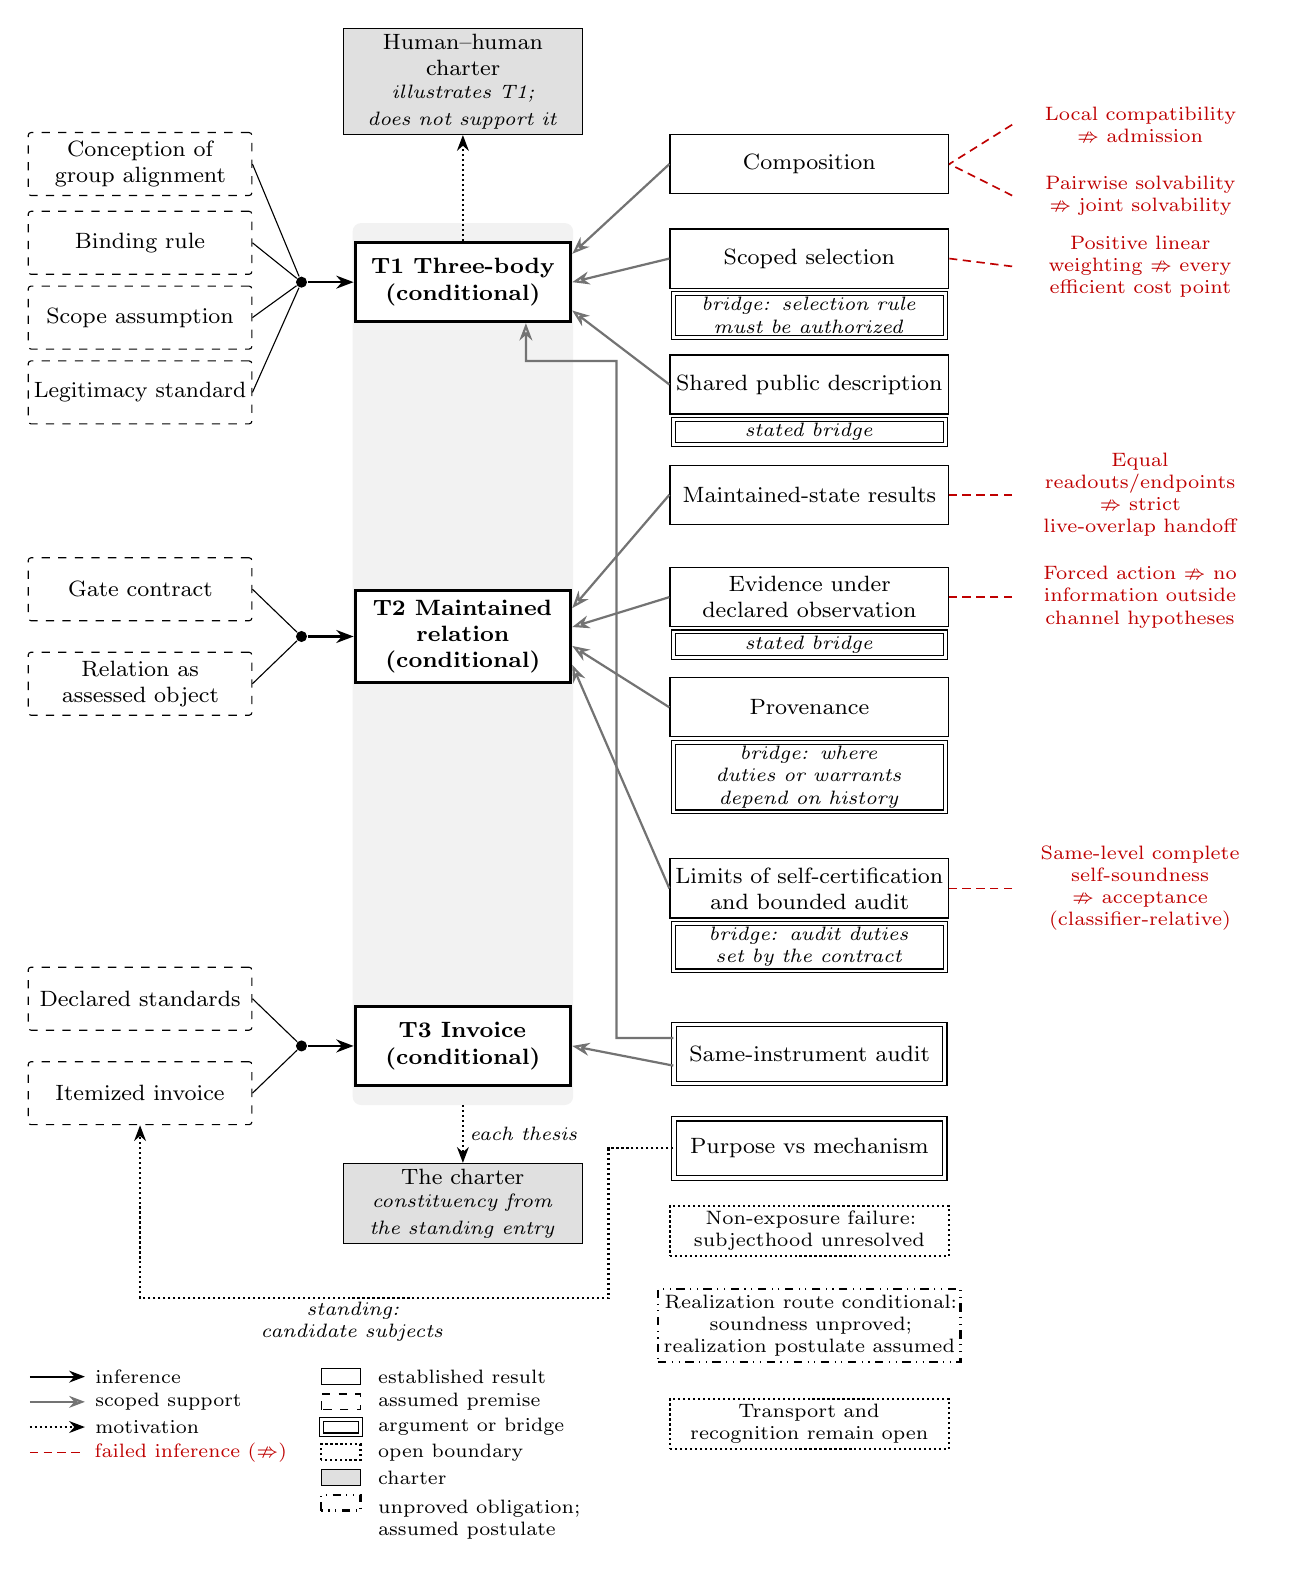
\begin{tikzpicture}[
  font=\footnotesize,
  execute at begin node={\hyphenpenalty=10000\exhyphenpenalty=10000},
  premise/.style={draw, dashed, rounded corners=1pt, align=center, text width=2.7cm, minimum height=0.8cm, inner sep=2pt},
  conjunction/.style={circle, fill=black, inner sep=0pt, minimum size=4pt},
  thesis/.style={draw, very thick, fill=white, align=center, text width=2.5cm, minimum height=1.0cm, font=\footnotesize\bfseries},
  family/.style={draw, align=center, text width=3.4cm, minimum height=0.75cm, inner sep=2pt},
  failed/.style={align=center, text width=3.0cm, text=red!75!black, font=\scriptsize},
  argument/.style={draw, double, double distance=1.2pt, align=center, text width=3.3cm, minimum height=0.75cm, inner sep=2pt},
  argument_cs/.style={argument},
  bridge/.style={draw, double, double distance=1pt, align=center, text width=3.35cm, inner sep=1.5pt, font=\scriptsize\itshape},
  boundary/.style={draw, densely dotted, thick, align=center, text width=3.4cm, minimum height=0.6cm, inner sep=2pt, font=\scriptsize},
  qualification/.style={draw, dash dot dot, thick, align=center, text width=3.7cm, minimum height=0.6cm, inner sep=2pt, font=\scriptsize},
  covenant/.style={draw, fill=black!12, align=center, text width=2.9cm, minimum height=0.8cm, inner sep=2pt},
  rel member/.style={draw, thin},
  rel inf/.style={draw, thick, -{Stealth[length=2.2mm]}},
  rel sup/.style={draw, thick, black!55, -{Stealth[open, length=2.2mm]}},
  rel mot/.style={draw, densely dotted, thick, -{Stealth[length=2mm]}},
  rel constrains/.style={draw, semithick, red!75!black, densely dashed},
]
  \fill[black!5, rounded corners=3pt] (4.2,1.55) rectangle (7.0,12.75);
  \node[premise] (p_serve) at (1.5,13.5) {Conception of group alignment};
  \node[premise] (p_bind) at (1.5,12.5) {Binding rule};
  \node[premise] (p_scope) at (1.5,11.55) {Scope assumption};
  \node[premise] (p_e3) at (1.5,10.6) {Legitimacy standard};
  \node[premise] (p_ag) at (1.5,8.1) {Gate contract};
  \node[premise] (b_rel) at (1.5,6.9) {Relation as assessed object};
  \node[premise] (p_method) at (1.5,2.9) {Declared standards};
  \node[premise] (p_invoice) at (1.5,1.7) {Itemized invoice};
  \node[conjunction] (j1) at (3.55,12.0) {};
  \node[conjunction] (j2) at (3.55,7.5) {};
  \node[conjunction] (j3) at (3.55,2.3) {};
  \node[thesis] (t1) at (5.6,12.0) {T1 Three-body (conditional)};
  \node[thesis] (t2) at (5.6,7.5) {T2 Maintained relation (conditional)};
  \node[thesis] (t3) at (5.6,2.3) {T3 Invoice (conditional)};
  \node[family] (f_comp) at (10.0,13.5) {Composition};
  \node[family] (f_sel) at (10.0,12.3) {Scoped selection};
  \node[bridge, anchor=north] (f_sel_bridge) at ([yshift=-1.5pt]f_sel.south) {bridge: selection rule must be authorized};
  \node[family] (f_shared) at (10.0,10.7) {Shared public description};
  \node[bridge, anchor=north] (f_shared_bridge) at ([yshift=-1.5pt]f_shared.south) {stated bridge};
  \node[family] (f_state) at (10.0,9.3) {Maintained-state results};
  \node[family] (f_evid) at (10.0,8.0) {Evidence under declared observation};
  \node[bridge, anchor=north] (f_evid_bridge) at ([yshift=-1.5pt]f_evid.south) {stated bridge};
  \node[family] (f_prov) at (10.0,6.6) {Provenance};
  \node[bridge, anchor=north] (f_prov_bridge) at ([yshift=-1.5pt]f_prov.south) {bridge: where duties or warrants depend on history};
  \node[family] (f_audit) at (10.0,4.3) {Limits of self-certification and bounded audit};
  \node[bridge, anchor=north] (f_audit_bridge) at ([yshift=-1.5pt]f_audit.south) {bridge: audit duties set by the contract};
  \node[argument] (f_au) at (10.0,2.2) {Same-instrument audit};
  \node[failed] (x2a) at (14.2,14.0) {Local compatibility $\nRightarrow$ admission};
  \node[failed] (x2b) at (14.2,13.1) {Pairwise solvability $\nRightarrow$ joint solvability};
  \node[failed] (x3) at (14.2,12.2) {Positive linear weighting $\nRightarrow$ every efficient cost point};
  \node[failed] (x10) at (14.2,9.3) {Equal readouts/endpoints $\nRightarrow$ strict live-overlap handoff};
  \node[failed] (x4) at (14.2,8.0) {Forced action $\nRightarrow$ no information outside channel hypotheses};
  \node[failed] (x16) at (14.2,4.3) {Same-level complete self-soundness $\nRightarrow$ acceptance (classifier-relative)};
  \node[argument_cs] (cs) at (10.0,1.0) {Purpose vs mechanism};
  \node[boundary] (cs_n2) at (10.0,-0.05) {Non-exposure failure: subjecthood unresolved};
  \node[qualification] (cs_h1) at (10.0,-1.25) {Realization route conditional: soundness unproved; realization postulate assumed};
  \node[boundary] (cs_tr) at (10.0,-2.5) {Transport and recognition remain open};
  \node[covenant] (k0) at (5.6,0.3) {The charter\\[-1pt]{\scriptsize\itshape constituency from the standing entry}};
  \node[covenant] (khh) at (5.6,14.55) {Human--human charter\\[-1pt]{\scriptsize\itshape illustrates T1; does not support it}};
  \path[rel member] (p_serve.east) -- (j1);
  \path[rel member] (p_bind.east) -- (j1);
  \path[rel member] (p_scope.east) -- (j1);
  \path[rel member] (p_e3.east) -- (j1);
  \path[rel inf] (j1) -- (t1.west);
  \path[rel member] (p_ag.east) -- (j2);
  \path[rel member] (b_rel.east) -- (j2);
  \path[rel inf] (j2) -- (t2.west);
  \path[rel member] (p_method.east) -- (j3);
  \path[rel member] (p_invoice.east) -- (j3);
  \path[rel inf] (j3) -- (t3.west);
  \path[rel sup] (f_comp.west) -- ([yshift=0.36cm]t1.east);
  \path[rel sup] (f_sel.west) -- ([yshift=0.00cm]t1.east);
  \path[rel sup] (f_shared.west) -- ([yshift=-0.36cm]t1.east);
  \path[rel sup] (f_state.west) -- ([yshift=0.36cm]t2.east);
  \path[rel sup] (f_evid.west) -- ([yshift=0.12cm]t2.east);
  \path[rel sup] (f_prov.west) -- ([yshift=-0.12cm]t2.east);
  \path[rel sup] (f_audit.west) -- ([yshift=-0.36cm]t2.east);
  \path[rel sup] ([yshift=-1.5mm]f_au.west) -- ([yshift=0.00cm]t3.east);
  \path[rel sup] ([yshift=2mm]f_au.west) -- (7.55,2.40) -- (7.55,11.0) -| ([xshift=0.8cm]t1.south);
  \path[rel constrains] (x2a.west) -- (f_comp.east);
  \path[rel constrains] (x2b.west) -- (f_comp.east);
  \path[rel constrains] (x3.west) -- (f_sel.east);
  \path[rel constrains] (x10.west) -- (f_state.east);
  \path[rel constrains] (x4.west) -- (f_evid.east);
  \path[rel constrains] (x16.west) -- (f_audit.east);
  \path[rel mot] (5.6,1.55) -- (k0.north) node[midway, right, font=\scriptsize\itshape, inner sep=2pt] {each thesis};
  \path[rel mot] (t1) -- (khh);
  \path[rel mot] (cs.west) -- (7.45,0 |- cs.west) -- (7.45,-0.9) -| (p_invoice.south);
  \node[font=\scriptsize\itshape, align=center, text width=3.0cm, inner sep=1pt] at (4.2,-1.2) {standing: candidate subjects};
  \begin{scope}[shift={(0.1,-1.9)}, font=\scriptsize]
    \draw[thick, -{Stealth[length=2mm]}] (0,0) -- (0.7,0) node[right, black] {inference};
    \draw[thick, black!55, -{Stealth[open, length=2mm]}] (0,-0.32) -- (0.7,-0.32) node[right, black] {scoped support};
    \draw[densely dotted, thick, -{Stealth[length=2mm]}] (0,-0.64) -- (0.7,-0.64) node[right] {motivation};
    \draw[red!75!black, densely dashed] (0,-0.96) -- (0.7,-0.96) node[right, text=red!75!black] {failed inference ($\nRightarrow$)};
  \end{scope}
  \begin{scope}[shift={(3.7,-1.9)}, font=\scriptsize]
    \draw (0.1,-0.1) rectangle (0.6,0.1); \node[right] at (0.7,0) {established result};
    \draw[dashed] (0.1,-0.42) rectangle (0.6,-0.22); \node[right] at (0.7,-0.32) {assumed premise};
    \draw[double, double distance=1pt] (0.1,-0.74) rectangle (0.6,-0.54); \node[right] at (0.7,-0.64) {argument or bridge};
    \draw[densely dotted, thick] (0.1,-1.06) rectangle (0.6,-0.86); \node[right] at (0.7,-0.96) {open boundary};
    \draw[fill=black!12] (0.1,-1.38) rectangle (0.6,-1.18); \node[right] at (0.7,-1.28) {charter};
    \draw[dash dot dot, thick] (0.1,-1.70) rectangle (0.6,-1.50); \node[right, text width=3.5cm, align=left, anchor=north west] at (0.7,-1.44) {unproved obligation; assumed postulate};
  \end{scope}
  \ifshowstubs\node[font=\scriptsize\itshape, text=black!45, anchor=north east] at (16.0,15.3) {scaffold layout (A8)};\fi
\end{tikzpicture}

  \caption{The argument map. Declared premises yield conditional theses; source results provide scoped support through stated bridges. The same-instrument audit is an interpretive argument. Crossed arrows show scoped failures. The purpose-versus-mechanism box motivates the invoice's standing entry, which fixes whom the charter protects. The charters are motivated proposals: the arrow from the foot of the shaded thesis column means that each thesis motivates the charter, and the human--human charter illustrates T1.}
  \label{fig:argument-map}
\end{figure}
\begin{table}[htbp]
  \centering\footnotesize
  \caption{Known versus new. ``Corpus'': results of \renderchoice{my earlier work}{Tsiokos's earlier work}, at their source grades. ``New here'': proposals, declared bridges and project mathematics, with certification in the Grade column. CL: claim rows.}
  \label{tab:claims}
  \tablerows
  \begin{tabularx}{\textwidth}{@{}>{\raggedright\arraybackslash}p{2.7cm}>{\raggedright\arraybackslash}X>{\raggedright\arraybackslash}X>{\raggedright\arraybackslash}p{3.0cm}@{}}
    \toprule
    Claim & Known (credit) & New here & Grade \\
    \midrule
    T1, three bodies (CL-60a to CL-61) & Whose principles \citep{gabriel2020}; a tetradic relation \citep{gabriel2024assistants}; intent alignment \citep{christiano2018clarifying}; normative infrastructure \citep{hadfieldmenell2019incomplete} & The scoped authorization requirement, derived from a binding rule, a conception of group alignment, a scope assumption and an adopted legitimacy standard & conditional argument from stated premises \\
    T2, maintained relation (CL-31, CL-63, CL-64) & Maintained accounts \citep{rahwan2018,zhixuan2025}; predictive states \citep{shalizi2001}; history-dependent rewards \citep{bacchus1996,toroicarte2018} & The gate contract; what assessment must preserve; the protected-duty reading of a credited pairing & proposal; kernel-checked repair lemmas; written/exact instance bridges \\
    T3, the invoice (CL-66, CL-67) & Standing and aggregation decisions \citep{baum2020} & Nine itemized standards with a refusal rule & this paper's proposal \\
    Composition and selection (CL-01 to CL-05) & Gluing; weighted sums \citep{ehrgott2005,harsanyi1955}; social choice for preference learning \citep{conitzer2024,ge2024} & Declared alignment readings of earlier corpus composition and selection limits & corpus theorems at stated grades \\
    Evidence, provenance and audit (CL-14 to CL-19; CL-32) & Machine experiments \citep{moore1956}; code distance \citep{hamming1950}; data processing \citep{cover2005}; self-trust \citep{yudkowsky2013tiling}; debate \citep{browncohen2024} & A finite-channel corollary of data processing under stated channel hypotheses; declared audit bridges & corpus grades; written channel theorem; interpretive bridges \\
    Who alignment is for (CL-20, CL-21, CL-35; CL-69 to CL-71) & Moral-status uncertainty \citep{schwitzgebel2015,long2024,butlin2023}; behaviour as evidence \citep{danaher2020}; closure architecture \citep{tsiokos2026consciousness} & Purpose/mechanism distinction; within-action-fiber privacy on inhabited products & argument; kernel-checked interface lemmas; written interpretation; conditional realization\textsuperscript{a} \\
    The covenant (CL-40 to CL-57) & Indirect reciprocity \citep{sugden1986,nowak1998,ohtsuki2004}; folk theorems \citep{fudenberg1986}; shutdown \citep{soares2015} & A charter; exact finite results with their failures & proposal; new results on declared models \\
    Obligation register (CL-34, CL-68) & Abstraction traps \citep{selbst2019} & What a mapping must supply; no verdicts & argument \\
    \bottomrule
  \end{tabularx}

  \smallskip
  {\footnotesize\raggedright
  \textsuperscript{a}\,Role-split privacy does not preserve original non-exposure at an accountable interface with distinct recoverable actions, nor guarantee statistical independence or future secrecy. It does not repair the realization certificate. The realization route assumes certificate soundness (unproved) and the realization postulate.\par}
\end{table}
\FloatBarrier%
\end{appendices}

\ifsnjnl\else\bibliographystyle{plainnat}\fi
\bibliography{references}

\end{document}
